% Generated by Sphinx.
\def\sphinxdocclass{report}
\documentclass[letterpaper,12pt,english]{sphinxmanual}
\usepackage[utf8]{inputenc}
\DeclareUnicodeCharacter{00A0}{\nobreakspace}
\usepackage{cmap}
\usepackage[T1]{fontenc}
\usepackage{babel}
\usepackage{times}
\usepackage[Bjarne]{fncychap}
\usepackage{longtable}
\usepackage{sphinx}
\usepackage{multirow}


\title{Manifestos of the Information Age: An Anthology}
\date{January 27, 2015}
\release{15.1.7}
\author{Various Authors}
\newcommand{\sphinxlogo}{
\includegraphics{internet_earth.png}\par}
\renewcommand{\releasename}{Release}
\makeindex

\makeatletter
\def\PYG@reset{\let\PYG@it=\relax \let\PYG@bf=\relax%
    \let\PYG@ul=\relax \let\PYG@tc=\relax%
    \let\PYG@bc=\relax \let\PYG@ff=\relax}
\def\PYG@tok#1{\csname PYG@tok@#1\endcsname}
\def\PYG@toks#1+{\ifx\relax#1\empty\else%
    \PYG@tok{#1}\expandafter\PYG@toks\fi}
\def\PYG@do#1{\PYG@bc{\PYG@tc{\PYG@ul{%
    \PYG@it{\PYG@bf{\PYG@ff{#1}}}}}}}
\def\PYG#1#2{\PYG@reset\PYG@toks#1+\relax+\PYG@do{#2}}

\expandafter\def\csname PYG@tok@gd\endcsname{\def\PYG@tc##1{\textcolor[rgb]{0.63,0.00,0.00}{##1}}}
\expandafter\def\csname PYG@tok@gu\endcsname{\let\PYG@bf=\textbf\def\PYG@tc##1{\textcolor[rgb]{0.50,0.00,0.50}{##1}}}
\expandafter\def\csname PYG@tok@gt\endcsname{\def\PYG@tc##1{\textcolor[rgb]{0.00,0.27,0.87}{##1}}}
\expandafter\def\csname PYG@tok@gs\endcsname{\let\PYG@bf=\textbf}
\expandafter\def\csname PYG@tok@gr\endcsname{\def\PYG@tc##1{\textcolor[rgb]{1.00,0.00,0.00}{##1}}}
\expandafter\def\csname PYG@tok@cm\endcsname{\let\PYG@it=\textit\def\PYG@tc##1{\textcolor[rgb]{0.25,0.50,0.56}{##1}}}
\expandafter\def\csname PYG@tok@vg\endcsname{\def\PYG@tc##1{\textcolor[rgb]{0.73,0.38,0.84}{##1}}}
\expandafter\def\csname PYG@tok@m\endcsname{\def\PYG@tc##1{\textcolor[rgb]{0.13,0.50,0.31}{##1}}}
\expandafter\def\csname PYG@tok@mh\endcsname{\def\PYG@tc##1{\textcolor[rgb]{0.13,0.50,0.31}{##1}}}
\expandafter\def\csname PYG@tok@cs\endcsname{\def\PYG@tc##1{\textcolor[rgb]{0.25,0.50,0.56}{##1}}\def\PYG@bc##1{\setlength{\fboxsep}{0pt}\colorbox[rgb]{1.00,0.94,0.94}{\strut ##1}}}
\expandafter\def\csname PYG@tok@ge\endcsname{\let\PYG@it=\textit}
\expandafter\def\csname PYG@tok@vc\endcsname{\def\PYG@tc##1{\textcolor[rgb]{0.73,0.38,0.84}{##1}}}
\expandafter\def\csname PYG@tok@il\endcsname{\def\PYG@tc##1{\textcolor[rgb]{0.13,0.50,0.31}{##1}}}
\expandafter\def\csname PYG@tok@go\endcsname{\def\PYG@tc##1{\textcolor[rgb]{0.20,0.20,0.20}{##1}}}
\expandafter\def\csname PYG@tok@cp\endcsname{\def\PYG@tc##1{\textcolor[rgb]{0.00,0.44,0.13}{##1}}}
\expandafter\def\csname PYG@tok@gi\endcsname{\def\PYG@tc##1{\textcolor[rgb]{0.00,0.63,0.00}{##1}}}
\expandafter\def\csname PYG@tok@gh\endcsname{\let\PYG@bf=\textbf\def\PYG@tc##1{\textcolor[rgb]{0.00,0.00,0.50}{##1}}}
\expandafter\def\csname PYG@tok@ni\endcsname{\let\PYG@bf=\textbf\def\PYG@tc##1{\textcolor[rgb]{0.84,0.33,0.22}{##1}}}
\expandafter\def\csname PYG@tok@nl\endcsname{\let\PYG@bf=\textbf\def\PYG@tc##1{\textcolor[rgb]{0.00,0.13,0.44}{##1}}}
\expandafter\def\csname PYG@tok@nn\endcsname{\let\PYG@bf=\textbf\def\PYG@tc##1{\textcolor[rgb]{0.05,0.52,0.71}{##1}}}
\expandafter\def\csname PYG@tok@no\endcsname{\def\PYG@tc##1{\textcolor[rgb]{0.38,0.68,0.84}{##1}}}
\expandafter\def\csname PYG@tok@na\endcsname{\def\PYG@tc##1{\textcolor[rgb]{0.25,0.44,0.63}{##1}}}
\expandafter\def\csname PYG@tok@nb\endcsname{\def\PYG@tc##1{\textcolor[rgb]{0.00,0.44,0.13}{##1}}}
\expandafter\def\csname PYG@tok@nc\endcsname{\let\PYG@bf=\textbf\def\PYG@tc##1{\textcolor[rgb]{0.05,0.52,0.71}{##1}}}
\expandafter\def\csname PYG@tok@nd\endcsname{\let\PYG@bf=\textbf\def\PYG@tc##1{\textcolor[rgb]{0.33,0.33,0.33}{##1}}}
\expandafter\def\csname PYG@tok@ne\endcsname{\def\PYG@tc##1{\textcolor[rgb]{0.00,0.44,0.13}{##1}}}
\expandafter\def\csname PYG@tok@nf\endcsname{\def\PYG@tc##1{\textcolor[rgb]{0.02,0.16,0.49}{##1}}}
\expandafter\def\csname PYG@tok@si\endcsname{\let\PYG@it=\textit\def\PYG@tc##1{\textcolor[rgb]{0.44,0.63,0.82}{##1}}}
\expandafter\def\csname PYG@tok@s2\endcsname{\def\PYG@tc##1{\textcolor[rgb]{0.25,0.44,0.63}{##1}}}
\expandafter\def\csname PYG@tok@vi\endcsname{\def\PYG@tc##1{\textcolor[rgb]{0.73,0.38,0.84}{##1}}}
\expandafter\def\csname PYG@tok@nt\endcsname{\let\PYG@bf=\textbf\def\PYG@tc##1{\textcolor[rgb]{0.02,0.16,0.45}{##1}}}
\expandafter\def\csname PYG@tok@nv\endcsname{\def\PYG@tc##1{\textcolor[rgb]{0.73,0.38,0.84}{##1}}}
\expandafter\def\csname PYG@tok@s1\endcsname{\def\PYG@tc##1{\textcolor[rgb]{0.25,0.44,0.63}{##1}}}
\expandafter\def\csname PYG@tok@gp\endcsname{\let\PYG@bf=\textbf\def\PYG@tc##1{\textcolor[rgb]{0.78,0.36,0.04}{##1}}}
\expandafter\def\csname PYG@tok@sh\endcsname{\def\PYG@tc##1{\textcolor[rgb]{0.25,0.44,0.63}{##1}}}
\expandafter\def\csname PYG@tok@ow\endcsname{\let\PYG@bf=\textbf\def\PYG@tc##1{\textcolor[rgb]{0.00,0.44,0.13}{##1}}}
\expandafter\def\csname PYG@tok@sx\endcsname{\def\PYG@tc##1{\textcolor[rgb]{0.78,0.36,0.04}{##1}}}
\expandafter\def\csname PYG@tok@bp\endcsname{\def\PYG@tc##1{\textcolor[rgb]{0.00,0.44,0.13}{##1}}}
\expandafter\def\csname PYG@tok@c1\endcsname{\let\PYG@it=\textit\def\PYG@tc##1{\textcolor[rgb]{0.25,0.50,0.56}{##1}}}
\expandafter\def\csname PYG@tok@kc\endcsname{\let\PYG@bf=\textbf\def\PYG@tc##1{\textcolor[rgb]{0.00,0.44,0.13}{##1}}}
\expandafter\def\csname PYG@tok@c\endcsname{\let\PYG@it=\textit\def\PYG@tc##1{\textcolor[rgb]{0.25,0.50,0.56}{##1}}}
\expandafter\def\csname PYG@tok@mf\endcsname{\def\PYG@tc##1{\textcolor[rgb]{0.13,0.50,0.31}{##1}}}
\expandafter\def\csname PYG@tok@err\endcsname{\def\PYG@bc##1{\setlength{\fboxsep}{0pt}\fcolorbox[rgb]{1.00,0.00,0.00}{1,1,1}{\strut ##1}}}
\expandafter\def\csname PYG@tok@kd\endcsname{\let\PYG@bf=\textbf\def\PYG@tc##1{\textcolor[rgb]{0.00,0.44,0.13}{##1}}}
\expandafter\def\csname PYG@tok@ss\endcsname{\def\PYG@tc##1{\textcolor[rgb]{0.32,0.47,0.09}{##1}}}
\expandafter\def\csname PYG@tok@sr\endcsname{\def\PYG@tc##1{\textcolor[rgb]{0.14,0.33,0.53}{##1}}}
\expandafter\def\csname PYG@tok@mo\endcsname{\def\PYG@tc##1{\textcolor[rgb]{0.13,0.50,0.31}{##1}}}
\expandafter\def\csname PYG@tok@mi\endcsname{\def\PYG@tc##1{\textcolor[rgb]{0.13,0.50,0.31}{##1}}}
\expandafter\def\csname PYG@tok@kn\endcsname{\let\PYG@bf=\textbf\def\PYG@tc##1{\textcolor[rgb]{0.00,0.44,0.13}{##1}}}
\expandafter\def\csname PYG@tok@o\endcsname{\def\PYG@tc##1{\textcolor[rgb]{0.40,0.40,0.40}{##1}}}
\expandafter\def\csname PYG@tok@kr\endcsname{\let\PYG@bf=\textbf\def\PYG@tc##1{\textcolor[rgb]{0.00,0.44,0.13}{##1}}}
\expandafter\def\csname PYG@tok@s\endcsname{\def\PYG@tc##1{\textcolor[rgb]{0.25,0.44,0.63}{##1}}}
\expandafter\def\csname PYG@tok@kp\endcsname{\def\PYG@tc##1{\textcolor[rgb]{0.00,0.44,0.13}{##1}}}
\expandafter\def\csname PYG@tok@w\endcsname{\def\PYG@tc##1{\textcolor[rgb]{0.73,0.73,0.73}{##1}}}
\expandafter\def\csname PYG@tok@kt\endcsname{\def\PYG@tc##1{\textcolor[rgb]{0.56,0.13,0.00}{##1}}}
\expandafter\def\csname PYG@tok@sc\endcsname{\def\PYG@tc##1{\textcolor[rgb]{0.25,0.44,0.63}{##1}}}
\expandafter\def\csname PYG@tok@sb\endcsname{\def\PYG@tc##1{\textcolor[rgb]{0.25,0.44,0.63}{##1}}}
\expandafter\def\csname PYG@tok@k\endcsname{\let\PYG@bf=\textbf\def\PYG@tc##1{\textcolor[rgb]{0.00,0.44,0.13}{##1}}}
\expandafter\def\csname PYG@tok@se\endcsname{\let\PYG@bf=\textbf\def\PYG@tc##1{\textcolor[rgb]{0.25,0.44,0.63}{##1}}}
\expandafter\def\csname PYG@tok@sd\endcsname{\let\PYG@it=\textit\def\PYG@tc##1{\textcolor[rgb]{0.25,0.44,0.63}{##1}}}

\def\PYGZbs{\char`\\}
\def\PYGZus{\char`\_}
\def\PYGZob{\char`\{}
\def\PYGZcb{\char`\}}
\def\PYGZca{\char`\^}
\def\PYGZam{\char`\&}
\def\PYGZlt{\char`\<}
\def\PYGZgt{\char`\>}
\def\PYGZsh{\char`\#}
\def\PYGZpc{\char`\%}
\def\PYGZdl{\char`\$}
\def\PYGZhy{\char`\-}
\def\PYGZsq{\char`\'}
\def\PYGZdq{\char`\"}
\def\PYGZti{\char`\~}
% for compatibility with earlier versions
\def\PYGZat{@}
\def\PYGZlb{[}
\def\PYGZrb{]}
\makeatother

\begin{document}

\maketitle
\tableofcontents
\phantomsection\label{index::doc}



\chapter{Coming to Terms}
\label{preface:coming-to-terms}\label{preface::doc}\label{preface:manifestos-for-the-information-age-an-anthology}

\section{Understanding Manifestos}
\label{preface:understanding-manifestos}
A manifesto is a published verbal declaration of the intentions, motives, or views of the issuer, be it an individual, group, political party or government. A manifesto usually accepts a previously published opinion or public consensus and/or promotes a new idea with prescriptive notions for carrying out changes the author believes should be made. It often is political or artistic in nature, but may present an individual's life stance.


\section{Understanding ``Hackers''}
\label{preface:understanding-hackers}
\emph{Forthcoming, The Johns Hopkins Encyclopedia of Digital Textuality (E. Gabriella Coleman)}


\subsection{Introduction}
\label{preface:introduction}
Generally,
a
hacker
is
a
technologist
with
a
penchant
for
computing
and
a
hack
is
a
clever
technical
solution
arrived
at
through
non
-
obvious
means (Levy
1984,
Turkle
2005).

It
is
telling
that
a
hack,
as
defined
by
the
Hacker
Jargon
File, can mean the complete opposite of an ingenious intervention: a clunky, ugly fix,
that nevertheless completes the job at hand.

Among hackers, the term is often worn as a badge of honor. In the popular press, however, the
connotations
of
hacker
are
often
negative,
or
at
minimum
refer
to
illegal
intrusion
of
computer
systems.

These
differences
point
to
the
various
meanings and
histories associated with the
terms
\emph{hacker}
and
\emph{hacking}.

Hackers
tend
to
uphold
a
cluster
of
values:
freedom,
privacy,
and
access.

They
adore
computers
and
networks.

They are
trained
in
the
specialized — and economically lucrative — technical arts of programming,
system/network
administration,
and
security.

Some
gain
unauthorized
access
to
technologies (though much hacking is legal).

Foremost, hacking,
in
its
different
incarnations,
embodies
an
aesthetic
where
craftsmanship
and
craftiness
converge; hackers value
playfulness,
pranking
and
cleverness,
and
will
frequently
display
their
wit
through
source
code,
humor,
or
both.

But once
one
confronts
hacking historically and sociologically,
this
shared
plane
melts
into
a
sea
of
differences
that
have, until recently,
been
overlooked
in
the
literature
on
hacking
(Coleman
and
Golub
2008,
Jordan
2008).


\subsection{Rethinking the Story of the Hacker Ethic, from Single-Origin to Multiple Origins}
\label{preface:rethinking-the-story-of-the-hacker-ethic-from-single-origin-to-multiple-origins}
The
term
hacker
was
first
used
consistently
in
the
1960s
among
technologists
at
MIT
whose
lives
maniacally
revolved
around
making,
using
and
improving
computer
software — a
preoccupation that
Steven
Levy
dubbed
“a daring symbiosis between man
and
machine” in his
engaging 1984 account
\emph{Hackers: Heroes of the Computer Revolution} (1984: 39).

Levy
unbundled
the
groups’
unstated
ethical
codes
from
their
passionate,
everyday
collective
pursuits
and
conceptualized
them
as “the
hacker
ethic,”
shorthand for a mix
of
aesthetic
and
pragmatic
imperatives that included:
\begin{itemize}
\item {} 
commitment to information freedom,

\item {} 
mistrust of authority,

\item {} 
heightened dedication to meritocracy,

\item {} 
and the firm belief that computers can be the basis for beauty and a better world (1984: 39-46).

\end{itemize}

Levy’s
book
not
only
represented
what
had
been,
at
the
time,
an
esoteric
community but
also
inspired
others
to
identify
with
the
moniker
“hacker”
and
its
ethical
principles.

By
the
1980s,
many
other
technologists
routinely deployed
the
term
\emph{hacker,}
individuals
enthralled
with
tinkering
and
technical spelunking
but
whose
history
and
politics
were distinct
from those chronicled by Levy.

Sometimes
referred
to
as
the
“hacker underground,”
the story goes that they arose in the 1980s, sullying what had been a pristine and legal tradition. What is often overlooked is
their history: their heirs
are the
phone
phreaks
who
existed at the same time as the
first crop of university hackers
in
the
late
1950s
and
early
1960s.

These phreaks, as they were
eventually known,
tapped
into
the
phone
system
to
make
free
phone
calls,
explored \emph{The System,} and
found
each
other
on
phone
conferences
also
known
as
party
lines
(Sterling
1992, Rosenbaum 1971, Thomas
2003).

The
end
of
the
analog
phone
network
after the divestiture of “Ma Bell”
heralded
the
end
of
the
golden
age
of
phreaking, which was largely
replaced
with
the
exploration
of
computer
networks.

The marriage
between phreaking
and computer hacking
was
represented
in
the
popular
e-zine
\emph{Phrack},
first
published
in
1985
on
Bulletin
Boards
Systems,
where
hackers
of
all
kinds
congregated
(Scott
2005,
Sterling
1992,
Thomas
2002).

Hackers
in this vein
would
continue
to
publish
prolifically
in diverse
genres,
including
manifestos
(most famously “The
Conscience
of
a
Hacker”),
textfiles
(written
in
sparse
ASCII
text
but
often
filled
with
ASCII art,
audaciously
worded
content)
and
zines
(such as \emph{Hack-Tic} in
the
Netherlands
and
\emph{2600}
in
the
United
States).

By the
1990s, they
were
routinely
meeting
during
annual
hacker
“cons”
(Coleman
2010).

Although
many
of
these
underground
hackers
engaged
in
technical
exploration,
often scouting for
security
vulnerabilities,
they
also
sought
forbidden
fruit and their
actions
included
mockery,
spectacle,
and
transgression—a
politics
and
ethics
distinct
from
the
university
hackers
of
MIT,
Carnegie
Mellon,
and
Stanford
(although
there
was
plenty
of
pranking
and irreverence
among
these
hackers).

The canonical narrative identifying MIT as hackings’ first homeland — a place where the hacker ethic was born — is complicated when we account for other traditions such as phreaking,
which existed independently of university-based hacker communities, and shaped a subversive tradition that flourished in the 1980s and 1990s, only to change with the rise of the security industry and new laws criminalizing computer break-ins.

Instead of
locating a
single point of origin
for hacking, we should be attentive to \emph{multiple origins, distinct lineages and variable ethics.}


\subsection{The Politics of Naming}
\label{preface:the-politics-of-naming}
By the late 1980s, although various instances of hacking existed,
this more subversive
tradition became
the
public face of hacking, cemented, and sometimes distorted
by, media
accounts.
Some
hackers,
concerned
by
the
illicit
actions
of
other
hackers
and
negative,
sensationalist
media
portrayals,
started
to
call those who hacked for illegal or malicious purposes,
“crackers”
(Nissenbaum
2004).

The use of “cracker” was a
linguistic attempt to reclaim and sanitize
“hacker.” Unsurprisingly, many hackers also questioned the term.

As more automation tools became available, many also started to use the derogatory terms “script kiddies” to designate those who use scripts to circumvent computer security or deface websites, rather than finding a unique
compromise. It is a scornful term (no one would elect to self-designate as such) that demarcates boundaries, signals appropriate behavior, and gives voice to the value placed on ingenuity, inventiveness and self-sufficiency.

To this day, debate rages among technologists: who deserves the title of “hacker”?

What constitutes its parameters? Some readily accept variability, while others starkly demarcate borders.

When asked, many
are
ready
to
fire
off
definitions.
When
interviewed,
two
hackers distinguished
between
builders — often
found
in
free
and
open-source
communities
whose
lineage
goes
back
to
the
university
communities explored in Levy — and
breakers
with
whom
these hackers
identify.

They
define breakers as follows:

Di: I call
myself
a
hacker,
what
I
mean
is
that
I
apply
creativity
and
technical
knowledge
to
bypassing
defenses.

Da: Yeah I’ve
heard `obtaining lower level understanding
of a system
to bypass
systems'

...which
is
a
reasonable
definition.


\subsection{Genres of Hacking}
\label{preface:genres-of-hacking}
To
hackers
themselves,
“to
hack”
can
thus
mean
distinct
activities,
from
improving
the
Linux
operating
system
to
finding
vulnerabilities
and “fuzzing” for
exploits.

Some
distinctions
are
subtle,
while
others
are
profound
enough
to
warrant
thinking about hacking in terms of
genres with distinct aesthetics and histories
(Coleman
and
Golub
2008).

Free
and Open-Source hackers — those
that
have
used
legal
means
to
guarantee
perpetual
access
to
source
code — tend
to uphold
political
structures
of
transparency
(Coleman
2012c).

In contrast,
the
hacker
underground
is
more
opaque
in its
social
organization
(Thomas
2003).
These
hackers
have
made
secrecy
and
spectacle
into
a
high
art
form
(Coleman
2012b).

For decades
in Europe,
artistic practice
has been marshaled
for the sake of hackings (
Bazzichelli
2008,
Deseriis and Marano 2008).

Hardware
hacking
has
also
been
part
of
hacking for a long time.

Historically,
its
most
notable
manifestation
was
among
the
Homebrew
hackers
of
the
Bay
Area
who
hacked
one of
the
first
personal
computer
kits,
the
MITS
Altair
8800,
and
helped
fuel
a
nascent
personal
computer
industry.

Today,
hardware
hacking
is
exploding,
buoyed
by
the
spread
of
hack
spaces — physical
workshops
filled
with
tools
and
computers — across
North
America
and
Europe but also in Latin America and China.

Some
hackers
run
vibrant
political
collectives
whose
names, \emph{Riseup}
and
\emph{Mayfirst},
unabashedly
broadcast
their
technical
crusade
to
make
this
world
a
better
one
(Juris
2008,
Milberry
2012).

Other
politically-minded
hackers
have
gravitated
toward
Anonymous — an
umbrella
term
for
a
range
of
distinct and often unconnected
digital
operations —
to
engage
in
hacking
for
the
sake
of
leaking
sensitive
corporate
and
government
information
(Coleman
2012a
),
extending
a
longer
tradition
in
hacktivism
(Taylor
and
Jordan
2004).

Others — for
example, many “infosec”
(information
security)
hackers — are
first
and
foremost
committed
to
security,
and
tend
to
steer
clear
of
defining
their
actions
in
such
overtly
political
terms, even
if
hacking
tends
to
creep
into
political
territory.

Among those in the infosec community there are differences as to whether one should release a security vulnerability (often called full disclosure) or announce its existence without revealing details
(referred to as anti-disclosure).

A smaller, more extreme movement known as anti-sec, is vehemently against any disclosure, claiming that it is their “goal that, through mayhem and the destruction of all exploitative and detrimental communities, companies, and individuals, full disclosure will be abandoned and the security industry will be forced to reform.”

National andregional
differences
also make their mark.
Southern
European
hackers
have
articulated
a
more
leftist,
anarchist
commitment
than
their
northern
European
counterparts.

Recently,
nationalistic
hacking — though
virtually unexplored by
scholars — has
spread (Karatzogianni
2006
is
an
important
exception).
Pakistani
hackers
are
routinely
at
war
with
their
Indian
neighbors.
Chinese
hackers
are
quite
nationalistic
in
their
aims
and
aspirations
(Henderson
2007),
in
contrast
to
those
in
North
America,
Latin
America,
and
Europe,
whose
anti-authoritarian
stance
makes
many — though
certainly not
all — wary
of joining
government
endeavors.

It
would
be
a
mistake
to
treat
different types of hacking
as
cultural
cocoons.

Technical architectures, the language of codes, and protocols bring together different types of hackers and activities. For instance, as it was developed over the last four decades, the Unix Operating System, has worked to bind thousands of hackers together as part of what Chris Kelty calls a “recursive public” (2008).

While
we
can
say
that
hacker
action
and
ethical
principles
share
a
common
core or
general
ethos,
\emph{inquiry demonstrates that we can identify variance and even serious points of contention.}

Given
the
multi-faceted,
rich,
and
often
controversial
political
effects
engendered
by
hackers,
from
the
creation
of
new
licensing
regimes
to
exposing
the
abuses
of
the
surveillance
state
(Himanen
2001,
Söderberg
2008, Wark
2004) and
its historical dynamism,
it \emph{is imperative to keep the variations of hacking at the forefront of our inquiries.}


\subsection{Works Cited}
\label{preface:works-cited}\begin{itemize}
\item {} 
Bazzichelli, Tatiana. 2008 \emph{Networking, The Net as Artwork. Digital Aesthetics}. ResearchCenter: Aarhus University

\item {} 
Coleman, E. Gabriella. 2010. \emph{The Hacker Conference: A Ritual Condensation and Celebration of a Lifeworld}. Anthropological Quarterly. 83(1):47-72

\item {} 
2012a Our Weirdness is Free: The logic of Anonymous: Online Army, Agent of Chaos, and Seeker of Justice. Triple Canopy \href{http://canopycanopycanopy.com/15/our\_weirdness\_is\_free}{http://canopycanopycanopy.com/15/our\_weirdness\_is\_free}

\item {} 
2012b ``Phreaks, Hackers, and Trolls and the Politics of Transgression and Spectacle.'' In {\color{red}\bfseries{}*}The Social Media Reader. Michael Mandiberg, ed. New York: NYU Press

\item {} 
2012c Coding Freedom: The Ethics and Aesthetics of Hacking. Princeton: Princeton University Press.

\item {} 
Coleman, Gabriella and Golub Alex 2008 ``Hacker Practice: Moral Genres and the Cultural Articulation of Liberalism.” Anthropological Theory, Vol. 8, No. 3, 255-277.

\item {} 
Deseriis, Marco. and G. Marano 2008 Net.Art: L’arte della Connessione (Net.Art: The Art of Connecting) Milan: Shake. (First edition 2003)

\item {} 
Henderson, Scott 2007 The Dark Visitor: Inside the World of Chinese Hackers. Lulu.com

\item {} 
Himanen,Pekka 2001 The Hacker Ethic and the Spirit of the Information Age. New York: Random House.

\item {} 
Jordan, Tim 2008 Hacking: Digital Media and Technological Determinism. Cambridge: Polity Press.

\item {} 
Jordan, Tim and Paul Taylor 2004 Hacktivism and Cyberwars: Rebels with a Cause? London: Routledge.

\item {} 
Juris, Jeff 2008 Networking Futures. Durham: Duke University Press.

\item {} 
Kelty, Chris M. 2008 Two Bits: The Cultural Significance of Free Software. Durham: Duke University Press.

\item {} 
Karatzogianni, Athina 2006 The Politics of Cyberconflict. Routledge: London and New York.

\item {} 
Levy, Steven 1984 Hackers Heroes of the Computer Revolution. New York: Delta.

\item {} 
Milberry, Kate 2012 “Hacking for social justice: The politics of prefigurative technology. ”In (Re)Inventing the Internet: Critical Case Studies. Andrew Feenberg and Norm Friesen, editors. Rotterdam, The Netherlands: Sense Publishers.

\item {} 
Nissenbaum, Helen 2004 “Hackers and the Contested Ontology of Cyberspace.” New Media and Society (6)2:195-217.

\item {} 
Rosenbaum, Ron 1971 Secrets of the Little Blue Box. Esquire Magazine. \href{http://www.webcrunchers.com/crunch/stories/esq-art.html}{http://www.webcrunchers.com/crunch/stories/esq-art.html}

\item {} 
Scott, Jason 2005 BBS: The Documentary. \href{http://www.bbsdocumentary.com/}{http://www.bbsdocumentary.com/}

\item {} 
Söderberg, Johan 2008 Hacking Capitalism: The Free and Open Source Software Movement. London: Routledge.

\item {} 
Sterling, Bruce 1992 The Hacker Crackdown: Law and Disorder on the Electronic Frontier. New York: Bantam.

\item {} 
Thomas, Douglas 2002 Hacker Culture. Minneapolis: University of Minnesota Press.

\item {} 
Turkle, Sherry 2005 The Second Self: Computers and the Human Spirit, Twentieth Anniversary Edition. Cambridge: MIT Press.

\item {} 
Wark, Ken 2004 A Hacker Manifesto. Cambridge: Harvard University Press.

\end{itemize}


\chapter{Computer Networking Timeline}
\label{network-timeline:computer-networking-timeline}\label{network-timeline::doc}

\section{Internet Adoption}
\label{network-timeline:internet-adoption}
\scalebox{0.750000}{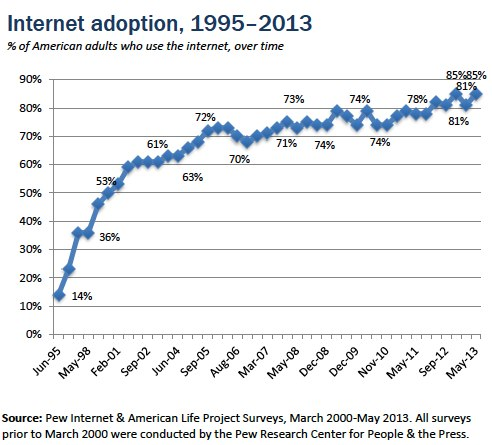
\includegraphics{adoption.jpg}}


\section{Internet Timeline}
\label{network-timeline:internet-timeline}

\subsection{1969}
\label{network-timeline:id1}
ARPA (Advanced Research Projects Agency) goes online in December, connecting four major U.S. universities. Designed for research, education, and government organizations, it provides a communications network linking the country in the event that a military attack destroys conventional communications systems.


\subsection{1972}
\label{network-timeline:id2}
Electronic mail is introduced by Ray Tomlinson, a Cambridge, Mass., computer scientist. He uses the @ to distinguish between the sender's name and network name in the email address.


\subsection{1973}
\label{network-timeline:id3}
Transmission Control Protocol/Internet Protocol (TCP/IP) is designed and in 1983 it becomes the standard for communicating between computers over the Internet. One of these protocols, FTP (File Transfer Protocol), allows users to log onto a remote computer, list the files on that computer, and download files from that computer.


\subsection{1976}
\label{network-timeline:id4}
Presidential candidate Jimmy Carter and running mate Walter Mondale use email to plan campaign events.

Queen Elizabeth sends her first email. She's the first state leader to do so.


\subsection{1982}
\label{network-timeline:id5}
The word “Internet” is used for the first time.


\subsection{1984}
\label{network-timeline:id6}
Domain Name System (DNS) is established, with network addresses identified by extensions such as .com, .org, and .edu.

Writer William Gibson coins the term “cyberspace.”


\subsection{1985}
\label{network-timeline:id7}
Quantum Computer Services, which later changes its name to America Online, debuts. It offers email, electronic bulletin boards, news, and other information.


\subsection{1988}
\label{network-timeline:id8}
A virus called the Internet Worm temporarily shuts down about 10\% of the world's Internet servers.


\subsection{1989}
\label{network-timeline:id9}
The World (world.std.com) debuts as the first provider of dial-up Internet access for consumers.

Tim Berners-Lee of CERN (European Laboratory for Particle Physics) develops a new technique for distributing information on the Internet. He calls it the World Wide Web. The Web is based on hypertext, which permits the user to connect from one document to another at different sites on the Internet via hyperlinks (specially programmed words, phrases, buttons, or graphics). Unlike other Internet protocols, such as FTP and email, the Web is accessible through a graphical user interface.


\subsection{1990}
\label{network-timeline:id10}
The first effort to index the Internet is created by Peter Deutsch at McGill University in Montreal, who devises Archie, an archive of FTP sites.


\subsection{1991}
\label{network-timeline:id11}
Gopher, which provides point-and-click navigation, is created at the University of Minnesota and named after the school mascot. Gopher becomes the most popular interface for several years.

Another indexing system, WAIS (Wide Area Information Server), is developed by Brewster Kahle of Thinking Machines Corp.


\subsection{1993}
\label{network-timeline:id12}
Mosaic is developed by Marc Andreeson at the National Center for Supercomputing Applications (NCSA). It becomes the dominant navigating system for the World Wide Web, which at this time accounts for merely 1\% of all Internet traffic.


\subsection{1994}
\label{network-timeline:id13}
The White House launches its website, www.whitehouse.gov.

Initial commerce sites are established and mass marketing campaigns are launched via email, introducing the term “spamming” to the Internet vocabulary.

Marc Andreessen and Jim Clark start Netscape Communications. They introduce the Navigator browser.


\subsection{1995}
\label{network-timeline:id14}
CompuServe, America Online, and Prodigy start providing dial-up Internet access.

Sun Microsystems releases the Internet programming language called Java.

The Vatican launches its own website, www.vatican.va.


\subsection{1996}
\label{network-timeline:id15}
Approximately 45 million people are using the Internet, with roughly 30 million of those in North America (United States and Canada), 9 million in Europe, and 6 million in Asia/Pacific (Australia, Japan, etc.). 43.2 million (44\%) U.S. households own a personal computer, and 14 million of them are online.


\subsection{1997}
\label{network-timeline:id16}
On July 8, 1997, Internet traffic records are broken as the NASA website broadcasts images taken by Pathfinder on Mars. The broadcast generates 46 million hits in one day.

The term “weblog” is coined. It’s later shortened to “blog.”


\subsection{1998}
\label{network-timeline:id17}
Google opens its first office, in California.


\subsection{1999}
\label{network-timeline:id18}
College student Shawn Fanning invents Napster, a computer application that allows users to swap music over the Internet.

The number of Internet users worldwide reaches 150 million by the beginning of 1999. More than 50\% are from the United States.

“E-commerce” becomes the new buzzword as Internet shopping rapidly spreads.

MySpace.com is launched.


\subsection{2000}
\label{network-timeline:id19}
To the chagrin of the Internet population, deviant computer programmers begin designing and circulating viruses with greater frequency. “Love Bug” and “Stages” are two examples of self-replicating viruses that send themselves to people listed in a computer user's email address book. The heavy volume of email messages being sent and received forces many infected companies to temporarily shut down their clogged networks.

The Internet bubble bursts, as the fountain of investment capital dries up and the Nasdaq stock index plunges, causing the initial public offering (IPO) window to slam shut and many dotcoms to close their doors.

America Online buys Time Warner for \$16 billion. It’s the biggest merger of all time.


\subsection{2001}
\label{network-timeline:id20}
Napster is dealt a potentially fatal blow when the 9th U.S. Circuit Court of Appeals in San Francisco rules that the company is violating copyright laws and orders it to stop distributing copyrighted music. The file-swapping company says it is developing a subscription-based service.

About 9.8 billion electronic messages are sent daily.

Wikipedia is created.


\subsection{2002}
\label{network-timeline:id21}
As of January, 58.5\% of the U.S. population (164.14 million people) uses the Internet. Worldwide there are 544.2 million users.

The death knell tolls for Napster after a bankruptcy judge ruled in September that German media giant Bertelsmann cannot buy the assets of troubled Napster Inc. The ruling prompts Konrad Hilbers, Napster CEO, to resign and lay off his staff.


\subsection{2003}
\label{network-timeline:id22}
It's estimated that Internet users illegally download about 2.6 billion music files each month.

Spam, unsolicited email, becomes a server-clogging menace. It accounts for about half of all emails. In December, President Bush signs the Controlling the Assault of Non-Solicited Pornography and Marketing Act of 2003 (CAN-SPAM Act), which is intended to help individuals and businesses control the amount of unsolicited email they receive.

Apple Computer introduces Apple iTunes Music Store, which allows people to download songs for 99 cents each.

Apple Computer introduces Apple iTunes Music Store, which allows people to download songs for 99 cents each.


\subsection{2004}
\label{network-timeline:id23}
Internet Worm, called MyDoom or Novarg, spreads through Internet servers. About 1 in 12 email messages are infected.

Online spending reaches a record high—\$117 billion in 2004, a 26\% increase over 2003.


\subsection{2005}
\label{network-timeline:id24}
YouTube.com is launched.


\subsection{2006}
\label{network-timeline:id25}
There are more than 92 million websites online.


\subsection{2007}
\label{network-timeline:id26}
Legal online music downloads triple to 6.7 million downloads per week.

Colorado Rockies' computer system crashes when it receives 8.5 million hits within the first 90 minutes of World Series ticket sales.

The online game, World of Warcraft, hits a milestone when it surpasses 9 million subscribers worldwide in July.


\subsection{2008}
\label{network-timeline:id27}
In a move to challenge Google's dominance of search and advertising on the Internet, software giant Microsoft offers to buy Yahoo for \$44.6 billion.

In a San Fransisco federal district court, Judge Jeffrey S. White orders the disabling of Wikileaks.org, a Web site that discloses confidential information. The case was brought by Julius Baer Bank and Trust, located in the Cayman Islands, after a disgruntled ex-employee allegedly provided Wikileaks with stolen documents that implicate the bank in asset hiding, money laundering, and tax evasion. Many web communities, who see the ruling as unconstitutional, publicized alternate addresses for the site and distributed bank documents through their own networks. In response, Judge White issues another order to stop the distribution of bank documents.

Microsoft is fined \$1.3 billion by the European Commission for further abusing its dominant market position, and failing to comply to their 2004 judgment, which ordered Microsoft to give competitors information necessary to operate with Windows. Since 2004, Microsoft has been fined a total of \$2.5 billion by the Commission for not adhering to their ruling.


\subsection{2012}
\label{network-timeline:id28}
A major protest online in January shakes up Congressional support for anti-Web piracy measures. The protest, including a 24-hour shutdown of the English-language Wikipedia site, is over two bills, the Stop Online Piracy Act in the House and the Protect IP Act in the Senate. The main goal of both bills is to stop illegal downloading and streaming of TV shows and movies online. The tech industry is concerned that the bills will give media companies too much power to shut down websites.


\subsection{2014}
\label{network-timeline:id29}
A coding error discovered in April in OpenSSL, encryption software that makes transactions between a computer and a remote secure, makes users vulnerable to having their usernames, passwords, and personal information stolen. Millions of banks, Internet commerce companies, email services, government sites, and social media sites rely on OpenSSL to conduct secure transactions. The coding error was made in 2012. Computer security experts encourage computer users to change their passwords.

\emph{Sources for this timeline include International Data Corporation, the W3C Consortium, Nielsen/NetRatings, and the Internet Society.}

\emph{Information Please® Database, © 2014 Pearson Education, Inc. All rights reserved.}


\chapter{1986: The Hacker Manifesto (The Mentor)}
\label{1986:the-hacker-manifesto-the-mentor}\label{1986::doc}

\section{Preface}
\label{1986:preface}
The Conscience of a Hacker, also called the Hacker Manifesto, was published in 1986. Loyd Blankenship aka The Mentor wrote it after his arrest and it got picked up by Phrack, and achieved fame since then.


\section{The Conscience of a Hacker}
\label{1986:the-conscience-of-a-hacker}
Another one got caught today, it's all over the papers. ``Teenager Arrested in Computer Crime Scandal'', ``Hacker Arrested after Bank Tampering''...

Damn kids. They're all alike.

But did you, in your three-piece psychology and 1950's technobrain, ever take a look behind the eyes of the hacker ? Did you ever wonder what made him tick, what forces shaped him, what may have molded him ?

I am a hacker, enter my world...

Mine is a world that begins with school... I'm smarter than most of the other kids, this crap they teach us bores me...

Damn underachiever. They're all alike.

I'm in junior high or high school. I've listened to teachers explain for the fifteenth time how to reduce a fraction. I understand it. ``No, Ms. Smith, I didn't show my work. I did it in my head...''

Damn kid. Probably copied it. They're all alike.

I made a discovery today. I found a computer. Wait a second, this is cool. It does what I want it to. If it makes a mistake, it's because I screwed it up. Not because it doesn't like me...

Or feels threatened by me...

Or thinks I'm a smart ass...

Or doesn't like teaching and shouldn't be here...

Damn kid. All he does is play games. They're all alike.

And then it happened... a door opened to a world... rushing through the phone line like heroin through an addict's veins, an electronic pulse is sent out, a refuge from the day-to-day incompetencies is sought... a board is found.

``This is it... this is where I belong...''
I know everyone here... even if I've never met them, never talked to them, may never hear from them again... I know you all...

Damn kid. Tying up the phone line again. They're all alike...

You bet your ass we're all alike... we've been spoon-fed baby food at school when we hungered for steak... the bits of meat that you did let slip through were pre-chewed and tasteless. We've been dominated by sadists, or ignored by the apathetic. The few that had something to teach found us willing pupils, but those few are like drops of water in the desert.

This is our world now... the world of the electron and the switch, the beauty of the baud. We make use of a service already existing without paying for what could be dirt-cheap if it wasn't run by profiteering gluttons, and you call us criminals. We explore... and you call us criminals. We seek after knowledge... and you call us criminals. We exist without skin color, without nationality, without religious bias... and you call us criminals. You build atomic bombs, you wage wars, you murder, cheat, and lie to us and try to make us believe it's for our own good, yet we're the criminals.

Yes, I am a criminal. My crime is that of curiosity. My crime is that of judging people by what they say and think, not what they look like. My crime is that of outsmarting you, something that you will never forgive me for.

I am a hacker, and this is my manifesto. You may stop this individual, but you can't stop us all... after all, we're all alike.

\index{the Mentor}\index{baud}\index{teaching}\index{high school}\index{hacker}\index{Loyd Blankenship}\index{Phrak}

\chapter{Mid 1988: Crypto Anarchist Manifesto (Timothy C. May)}
\label{1988:mid-1988-crypto-anarchist-manifesto-timothy-c-may}\label{1988::doc}\label{1988:index-0}
A specter is haunting the modern world, the specter of crypto anarchy.

Computer technology is on the verge of providing the ability for individuals and groups to communicate and interact with each other in a totally anonymous manner. Two persons may exchange messages, conduct business, and negotiate electronic contracts without ever knowing the True Name, or legal identity, of the other. Interactions over networks will be untraceable, via extensive re-routing of encrypted packets and tamper-proof boxes which implement cryptographic protocols with nearly perfect assurance against any tampering. Reputations will be of central importance, far more important in dealings than even the credit ratings of today. These developments will alter completely the nature of government regulation, the ability to tax and control economic interactions, the ability to keep information secret, and will even alter the nature of trust and reputation.

The technology for this revolution, and it surely will be both a social and economic revolution, has existed in theory for the past decade. The methods are based upon public-key encryption, zero-knowledge interactive proof systems, and various software protocols for interaction, authentication, and verification. The focus has until now been on academic conferences in Europe and the U.S., conferences monitored closely by the National Security Agency. But only recently have computer networks and personal computers attained sufficient speed to make the ideas practically realizable. And the next ten years will bring enough additional speed to make the ideas economically feasible and essentially unstoppable. High-speed networks, ISDN, tamper-proof boxes, smart cards, satellites, Ku-band transmitters, multi-MIPS personal computers, and encryption chips now under development will be some of the enabling technologies.

The State will of course try to slow or halt the spread of this technology, citing national security concerns, use of the technology by drug dealers and tax evaders, and fears of societal disintegration. Many of these concerns will be valid; crypto anarchy will allow national secrets to be trade freely and will allow illicit and stolen materials to be traded. An anonymous computerized market will even make possible abhorrent markets for assassinations and extortion. Various criminal and foreign elements will be active users of CryptoNet. But this will not halt the spread of crypto anarchy.

Just as the technology of printing altered and reduced the power of medieval guilds and the social power structure, so too will cryptologic methods fundamentally alter the nature of corporations and of government interference in economic transactions. Combined with emerging information markets, crypto anarchy will create a liquid market for any and all material which can be put into words and pictures. And just as a seemingly minor invention like barbed wire made possible the fencing-off of vast ranches and farms, thus altering forever the concepts of land and property rights in the frontier West, so too will the seemingly minor discovery out of an arcane branch of mathematics come to be the wire clippers which dismantle the barbed wire around intellectual property.

Arise, you have nothing to lose but your barbed wire fences !

\index{cryptography}\index{intellectual property}\index{Cryptonet}\index{transactions}\index{the State}\index{Timothy C. May}\index{Marx}\index{national security}\index{criminal}\index{crypto anarchy}

\chapter{1993: A Cypherpunk's Manifesto (Eric Hughes)}
\label{1993::doc}\label{1993:a-cypherpunk-s-manifesto-eric-hughes}\label{1993:index-0}
\emph{March 9, 1993}

Privacy is necessary for an open society in the electronic age. Privacy is not secrecy. A private matter is something one doesn't want the whole world to know, but a secret matter is something one doesn't want anybody to know. Privacy is the power to selectively reveal oneself to the world.

If two parties have some sort of dealings, then each has a memory of their interaction. Each party can speak about their own memory of this; how could anyone prevent it? One could pass laws against it, but the freedom of speech, even more than privacy, is fundamental to an open society; we seek not to restrict any speech at all. If many parties speak together in the same forum, each can speak to all the others and aggregate together knowledge about individuals and other parties. The power of electronic communications has enabled such group speech, and it will not go away merely because we might want it to.

Since we desire privacy, we must ensure that each party to a transaction have knowledge only of that which is directly necessary for that transaction. Since any information can be spoken of, we must ensure that we reveal as little as possible. In most cases personal identity is not salient. When I purchase a magazine at a store and hand cash to the clerk, there is no need to know who I am. When I ask my electronic mail provider to send and receive messages, my provider need not know to whom I am speaking or what I am saying or what others are saying to me; my provider only need know how to get the message there and how much I owe them in fees. When my identity is revealed by the underlying mechanism of the transaction, I have no privacy. I cannot here selectively reveal myself; I must always reveal myself.

Therefore, privacy in an open society requires anonymous transaction systems. Until now, cash has been the primary such system. An anonymous transaction system is not a secret transaction system. An anonymous system empowers individuals to reveal their identity when desired and only when desired; this is the essence of privacy.

Privacy in an open society also requires cryptography. If I say something, I want it heard only by those for whom I intend it. If the content of my speech is available to the world, I have no privacy. To encrypt is to indicate the desire for privacy, and to encrypt with weak cryptography is to indicate not too much desire for privacy. Furthermore, to reveal one's identity with assurance when the default is anonymity requires the cryptographic signature.

We cannot expect governments, corporations, or other large, faceless organizations to grant us privacy out of their beneficence. It is to their advantage to speak of us, and we should expect that they will speak. To try to prevent their speech is to fight against the realities of information. Information does not just want to be free, it longs to be free. Information expands to fill the available storage space. Information is Rumor's younger, stronger cousin; Information is fleeter of foot, has more eyes, knows more, and understands less than Rumor.

We must defend our own privacy if we expect to have any. We must come together and create systems which allow anonymous transactions to take place. People have been defending their own privacy for centuries with whispers, darkness, envelopes, closed doors, secret handshakes, and couriers. The technologies of the past did not allow for strong privacy, but electronic technologies do.

We the Cypherpunks are dedicated to building anonymous systems. We are defending our privacy with cryptography, with anonymous mail forwarding systems, with digital signatures, and with electronic money.

Cypherpunks write code. We know that someone has to write software to defend privacy, and since we can't get privacy unless we all do, we're going to write it. We publish our code so that our fellow Cypherpunks may practice and play with it. Our code is free for all to use, worldwide. We don't much care if you don't approve of the software we write. We know that software can't be destroyed and that a widely dispersed system can't be shut down.

Cypherpunks deplore regulations on cryptography, for encryption is fundamentally a private act. The act of encryption, in fact, removes information from the public realm. Even laws against cryptography reach only so far as a nation's border and the arm of its violence. Cryptography will ineluctably spread over the whole globe, and with it the anonymous transactions systems that it makes possible.

For privacy to be widespread it must be part of a social contract. People must come and together deploy these systems for the common good. Privacy only extends so far as the cooperation of one's fellows in society. We the Cypherpunks seek your questions and your concerns and hope we may engage you so that we do not deceive ourselves. We will not, however, be moved out of our course because some may disagree with our goals.

The Cypherpunks are actively engaged in making the networks safer for privacy. Let us proceed together apace.

Onward.

\emph{Eric Hughes} \textless{}\href{mailto:hughes@soda.berkeley.edu}{hughes@soda.berkeley.edu}\textgreater{}

\index{cypherpunk}\index{cryptography}\index{networks}\index{anonymity}\index{anonymous}\index{transactions}\index{Eric Hughes}\index{privacy}\index{secrets}\index{open society}

\chapter{1995: Manifesto for Bad Subjects in Cyberspace}
\label{1995::doc}\label{1995:manifesto-for-bad-subjects-in-cyberspace}\label{1995:index-0}

\section{Preface}
\label{1995:preface}

\subsection{Subject}
\label{1995:subject}
Digital Diaspora, Digital Community


\subsection{Description}
\label{1995:description}
The Bad Subjects Production Team, authors of the Manifesto for Bad Subjects in Cyberspace, are primariy concerned with communal production and relations in cyberspace. Reminding the reader that cyberspace is malleable and unpredictable, the Bad Subjects Production Team desire to create a digital space that opposes both liberal communal institutions and the exploitative forces of capital.


\subsection{Creator}
\label{1995:creator}
Bad Subjects Production Team


\subsection{Source}
\label{1995:source}
\href{http://bad.eserver.org/issues/1995/18/manifesto.html}{http://bad.eserver.org/issues/1995/18/manifesto.html}


\subsection{Publisher}
\label{1995:publisher}
\href{http://bad.eserver.org/}{http://bad.eserver.org/}


\subsection{Date}
\label{1995:date}
January 1995


\subsection{Rights}
\label{1995:rights}
Copyright © by Bad Subjects 1995. All rights reserved.


\section{Body}
\label{1995:body}
While communities in cyberspace might have radical potential, it is important to keep in mind that such potential is not inherent to the medium itself. Cyberspace is not itself a community; many types of communities exist on computer networks, most of which are nothing more than an extension of the kinds of routine interactions we expect to encounter in capitalism.


\subsection{Introduction}
\label{1995:introduction}
In September of 1993, the Bad Subjects Collective published `A Manifesto for Bad Subjects,' in which we offered a critique of existing leftist politics. We argued that the Left today is characterized by cynicism, an investment in multiculturalism which emphasizes separatism, and a desire to compensate for its ineffectiveness by celebrating victimization and marginalization. At that time, Bad Subjects was just beginning to establish a presence on the Internet by organizing an e-mail list and setting up a gopher site where an electronic version of our publication is available. Through these avenues, our manifesto reached an audience larger than we had ever imagined possible. We received responses from as far away as Russia and New Zealand; the manifesto was even taught in classes across the United States. It has now become clear that Bad Subjects identity and popularity are largely a result of our on-line presence. While hard copies of the publication continue to be circulated, the vast majority of our readers come to us through the Internet.

In the manifesto, we recommended that leftist politics be more relevant to our everyday lives; in this way, we hoped to suggest a new relationship between personal and political commitments. Because our everyday life as bad subjects takes place largely on the Net, we want to offer an example of how to put this recommendation into practice. Whereas the Internet was once just a way for us to disseminate our articles, it has now become an important social context for the exchange and development of what on-line users have dubbed badsubjectian ideas. In short, cyberspace has become both an organizing tool and meeting place for bad subjects. It has also come to resemble — in some ways — the kind of Utopian community we imagined in our original manifesto. What follows represents our collective effort to explore the radical potential of cyberspace, while acknowledging its limitations.


\subsection{Cyberspace and Global Capital}
\label{1995:cyberspace-and-global-capital}
Cyberspace is the technological fetish of the moment, just as the telephone, automobile, radio, and television once were. In this sense, cyberspace can be said to represent the next logical step in the expansion of the mass media. Throughout the 20th Century, leftists from the Frankfurt School to contemporary critics such as Douglas Kellner and Todd Gitlin have been debating whether the mass media are a progressive or reactionary force. There has always been a danger that the mass media will only function as propaganda for the ruling classes. But at the same time, independent uses of mass media by radical groups have been cited as examples of the subversive potential of cheap technologies which can help organize and inform the masses.

Popular histories of the Internet generally underscore its chaotic and seemingly unreal structure. An Esquire magazine guide to getting on-line (December, 1994) by Phil Patton is typical, describing a dizzying landscape...whose ruling philosophy is complexity theory — the happy belief that this chaos will all sort itself out somehow, someday, and meanwhile, hey, go with the flow. ARPANET, the seed from which the Internet grew, was one of the US Department of Defenses innumerable Cold-War projects. Pattons history of the Internet parallels that of most other popular accounts in noting that its military origins did not prevent it from being appropriated by civilians. As the net became a means of communication, Patton writes, on its margins, just as beside the railroad or blacktop, a new culture began to sprout. Despite its historical connection to American nationalist politics, the Internet is perceived to be a place where anarchy reigns: state-planning created the Internet, but has now lost control over it.

Discussions of the Internets radical potential have tended to focus on this anarchic quality. Commentators have celebrated the ways in which the Internet has frustrated attempts by centralized powers to steer its development in a particular direction. Understandably, leftists wary of state power have agreed with them. But celebrating the chaos of the Internet comes dangerously close to celebrating the so-called free market of capitalism. The free market is supposed to be a space of productive chaos inimical to regulation. Ideally it functions all by itself without any political or economic steering. The free market promotes individualism; indeed, it is thought to function best when it encompasses a great diversity of tastes and needs. Moreover, the free market is a fiction which disguises the web of unequal social relationships constituting it.

Substituting the word cyberspace for free market in these descriptions allows us to see that what we value about cyberspace resembles what the Left has criticized about capitalism. Like global capitalism, computer networks bring people together in alienation rather than solidarity. People who interact on-line are generally not privy to the way those networks are produced by actual people existing within a concrete economic order. Cyberspace is a commodity in the process of being produced by programmers, paid system operators, and a range of volunteers who parcel out memory to users, generate more complicated interactive data spaces, and maintain order on newsgroups, mailing lists, and FTP sites. The Net is not antithetical to the free market, to consumerism, or to alienated labor. After all, science fiction author William Gibson invented the term cyberspace to describe virtual reality in a future dominated by multinational corporations and wealthy elites who prey on a vast, international underclass.

While communities in cyberspace might have radical potential, it is important to keep in mind that such potential is not inherent to the medium itself. Cyberspace is not itself a community; many types of communities exist on computer networks, most of which are nothing more than an extension of the kinds of routine interactions we expect to encounter in capitalism. On Usenet and the World Wide Web, for example, we encounter thinner and thinner boundaries between personal expression, politics, and advertising. There are newsgroups devoted simply to job listings. On World Wide Web, you might click on a word in the middle of an article about progressive politics in Slovenia and find yourself linked to an infoblurb promoting tourism in Eastern Europe. On-line galleries exist in a number of locations for the purposes of selling art, music, or text. Thus, the Internet reflects the economic and social conditions that underpin it.

In our excitement over the Internets potential, we must be wary of buying into the ideology of the free market it mirrors. If we value the Internet because it is chaotic, decentered, and promotes individuality for its own sake, then it is only a matter of time before we start to value the free market for the same reasons.


\subsection{Democracy Is Not Utopia}
\label{1995:democracy-is-not-utopia}
Promises of a good society offered by cybernetic communication are familiar to us by now. They come out of what we might call the democratic Utopianism espoused by everyone from techno-anarchists like the staff of Mondo 2000 to self-styled conservative futurist Newt Gingrich. Like the fiction of a free market, on-line democratic Utopianism is heavily informed by a belief that unhindered personal expression is the measure of our social freedom.

In on-line democratic Utopianism, cyberspace community ends up emulating political communities in physical reality. Hence, the drawbacks of actually existing democracy as we know it in the United States are prevalent in computer networks: the middle- and upper-classes constitute the largest and most vocal group, promoting their own interests without having to pay attention to the needs and desires of the underclasses and disenfranchised groups. Much has been made, for example, of the way politicians, local governments, and special interest groups can have town hall meetings in virtual reality and hear from the people. But on the Net, after all, one pays for the privilege of participating in any town hall meeting. Moreover, cyberspace runs the risk of becoming individualist to the point of parody, where personal expression is overvalued so much that it is impossible to assert anything unless it begins with the cyberslang disclaimer IMO {[}in my opinion{]}.

An overemphasis on the personal has led to many of the problems leftists face today when they try to organize themselves as a mass community once more. Personal or identity politics have led to distrust of all groups which attempt to take a strong, unified stance which might appeal to mainstream society. Multiculturalism has helped Americans to modify their interpersonal relations — making it rude and often illegal to be racist or sexist — but it has also undermined our ability to view the political as political. Lacking a clear vision of politics which go beyond the personal, the Left shies away from any program or set of goals which assert that large numbers of people can change society for the better. Whose society are you talking about? the multiculturalist might ask. Hearing that this society is one we all share, the multiculturalist disgustedly replies, No such society exists, and if it did, it would be oppressive. Certainly this is the case if all politics are merely personal, since no two people can share the same life. But politics go beyond individual experience.

To bring about a more just society, the left must commit to a politics which validate personal identity while at the same time transcending it. For this reason, the potential for political community in cyberspace seems particularly salient. On a computer network, identity as we know it in our daily lives is altered. Because we cannot instantly see each other as races, genders, ages, etc., in a computer environment, peoples impulse to judge one another as such is hindered. We could never argue that these judgments do not occur, and certainly many people on-line make sure to identify themselves somewhere on the multiculturalist spectrum. Nevertheless, it is appropriate to assert that radical communities on-line would not fall out along the same lines as they might in physical reality.

Computer networks are, as many commentators have noted, global, or, at the very least, international. Indeed, since going on-line, the Bad Subjects mailing list and readers have been made up of people from around the world. A radical community in cyberspace would, therefore, be constituted by a population united by their desire to affect more than simply their cultural group or national region. Insofar as people can choose how, or if, to represent their (multicultural) identities on-line, cyberspace may provide the ultimate forum for performative identities. That is, a woman on-line might perform the identity of a man, and vice versa. In some ways, we might be tempted to celebrate this, arguing that such a performance undermines the allegedly fixed nature of race, gender, ethnicity, etc.. Such on-line performances take us, perhaps, a small step beyond multiculturalism as we now know it.

What remains fixed, however, are the sites from which on-line access is made available. E-mail address suffixes such as org {[}organization{]}, gov {[}government{]} and edu {[}education{]} locate the user within a system of commercial, state, and educational networks. Outside the United States, users are also identified by a country code in their suffix. Although anonymous servers exist which can erase users addresses, these are not entirely foolproof, and their use is limited. This suggests that while multicultural identities can be temporarily transcended (or reinscribed) in cyberspace, work — or class — identities cannot. Cyberspace identities may suggest a post-multicultural and post-national world, but they do not entirely escape their social context.


\subsection{The Use of Liberal `Safe Spaces'}
\label{1995:the-use-of-liberal-safe-spaces}
Built into the structure of any radical politics is an injunction to form communities. We know for certain that social change is dependent upon teamwork — and the kind of teams we form as radicals can, ideally, become the blueprints for what a better society might look like. Unfortunately, leftist and other radical communities are notorious for their instability and hypocrisy. In the late 60s, the New Left and civil rights movements spawned the womens movement precisely because, to women and their allies, sexist behavior in these movements seemed so clearly in conflict with their stated goals of equality and social justice. Subsequently, the womens movement and other civil rights groups of the 70s, 80s, and 90s have asserted that the personal is political in order to encourage continuity between political convictions and everyday actions.

The limitations of a multiculturalist position are, in part, the impetus behind our ongoing commitment to Bad Subjects. The project of Bad Subjects has always been to provide a forum for the discussion of leftist politics and, out of that, to build a political community and promote social change. While the hard-copy publication offers a place for people to articulate a substantial and coherent position on an aspect of contemporary culture, the on-line mailing list is a space where people can discuss, more informally, `political education for everyday life.' On the list, people debate the possible ways in which the Left might be more effective at both understanding and transforming contemporary society. It resembles, therefore, a kind of `safe space' or `support group' that allows for the free exchange of ideas and positions. While only a few list members may participate at any given time, the messages are `bounced' to the 200 or so people who currently subscribe to the list. Even when people do not agree with each other, one result is the on-going production of a `badsubjectian' position on whatever happens to be the topic at hand. The mailing list, therefore, collectively articulates a position (albeit sometimes a provisional one) on a topic. By participating, list members are acting in ways that suggest the kind of political community the Bad Subjects collective has always tried to work towards.

This kind of free exchange can have its limitations, however. As with any `safe space' there is a need to be aware of the extent to which containing political discussions within places like the mailing list can give us a false sense of our power to transform society. One problem is that the free exchange of ideas can quickly turn into a debate where every position is considered equally valid. While most people on the list are already committed to leftist politics, discussions occasionally become mired in the kind of individualism mentioned earlier, precluding the possibility of criticism or the articulation of a more coherent, and, ultimately, useful position. While a degree of `liberal pluralism' — where everyone's opinion is equally valued and respected — is necessary, and the safe space of the list allows for, and, indeed, promotes, such a dynamic, there is a time where a stand needs to be taken in order for any substantial change to be possible.

While discussions on the Bad Subjects mailing list may suggest a kind of collective politics, there is need to distinguish between the feeling of political community that a list can generate, and the ability to make productive use of that community to enact material changes in the world. As with any support group, there is, moreover, a need to leave the group behind and use the techniques and knowledge gained from the list in our lives outside of cyberspace. Indeed, there are many social and political changes that the list makes possible. The exchange of ideas can, and often does, promote a shift in consciousness that contains within itself real material effects. Many people on the list are students, professors, or writers, who use ideas and resources from the list, for example, to change the ways in which they teach and learn in their respective professions.

We need to create a balance between the liberal pluralism found in places like the mailing list and the kind of radical politics that can effectively transform society. There is nothing inherently radical, after all, about either multiculturalism or liberal pluralism. Indeed, both frequently reinforce — by creating `alternative' or `niche' markets — the structures of capitalism that we aim to dismantle. While it is, of course, important to be conscious of many social and political perspectives, we must also self-consciously maintain a position that opposes, rather than validates, the structures and ideology of capitalism.

The kinds of interactive discussions taking place on the mailing list break down the boundary between producers and consumers of ideas and actions. Our desire is not to merely reach a mass audience whom we can educate, in other words, but to encourage people to act in the world to effect real social change. We work to make possible a world in which on-line members are not merely passive recipients of `badsubjectian' ideas, but active agents helping us to articulate such a position and enact it in the world at large. Self-consciousness about the political potential of cyberspace is, thus, not an end in itself. We must leave the Net behind and use it only as an impetus for social change in the `real' material world.


\subsection{A Radical Program for Cyberspace}
\label{1995:a-radical-program-for-cyberspace}
Cyberspace community is just another form of community, with all its potential pitfalls and triumphs. The form that a community takes is ultimately not the point — but what you do with that community is. And this is why we believe that on-line and real life communities are not in opposition to one another, or in a hierarchical relationship. These communities exist in relation to each other, and are in the process of making each other quite different as a result of their relationship. Real communities may have invented cybercommunities, but at this point there are real communities and relationships which have been forged in cyberspace. Hence, cyberspace and real society are in a dialectical relationship — they mutually create and influence each other.

The materialist dialectic of Marxist tradition is often interpreted to mean a set of relationships in which materiality is the most important factor. This, as many theorists have pointed out, depends on how you define materiality. As much as cyberspace would seem to be the realm of ideas, hence non-material, one needs to remember that there is a materiality to cyberspace. If there were no such materiality, we could not assert that some people have access to it while others do not. Nor could we compare the structure of cyberspace to the structure of capitalism, which is a notoriously materialistic system. Like all raw materials, cyberspace is unequally distributed throughout the world. Hence cyberspace has materiality and an ideology — there are actual ports, machines, and RAM; and there are beliefs we have about it and ways we behave in it. Cybercommunity, like real life community, is a combination of raw materials and human conviviality.

It is therefore reasonable to assume that radical politics in cyberspace do have a relationship to practices in non-virtual reality. A radical political program in cyberspace would recommend actions intended to equalize access to its raw materials and information. It would promote localized and global participation in the maintenance of cyberspace society, or its structure and laws. Finally, it would open up avenues by which anti-capitalist thought might be disseminated and national boundaries eroded. All these actions would have as their intended goal the construction of a future, Utopian society in which human identities are global and people are united by a commitment to justice, shared labor, socialized property, and the peaceful resolution of conflicts.

For the present, cyberspace is in its infancy. In critical discussions, often we speak of potential ways cyberspace might develop as a technology and as a social force. To theorize cyberspace is also to imaginatively project ourselves as a society into the future. Cyberspace is more than just a system of computers; it is also a network of human relationships in the process of emerging. What is Utopian about cyberspace at this point in history is that its structure is obviously not entirely fixed. Perhaps, in deciding how we wish to organize the future of cyberspace, we can teach ourselves that, indeed, the future of human society is not fixed either. We can always choose to be different, and more importantly, we can always choose to be better. Like cyberspace itself, this manifesto is an invitation to remember that, as individuals and as a society, this choice is always ours.

\emph{Copyright © by Bad Subjects 1995. All rights reserved.}


\chapter{1996: A Declaration of the Independence of Cyberspace (John Perry Barlow)}
\label{1996::doc}\label{1996:a-declaration-of-the-independence-of-cyberspace-john-perry-barlow}
\emph{February 8, 1996}

Governments of the Industrial World, you weary giants of flesh and steel, I come from Cyberspace, the new home of Mind. On behalf of the future, I ask you of the past to leave us alone. You are not welcome among us. You have no sovereignty where we gather.

We have no elected government, nor are we likely to have one, so I address you with no greater authority than that with which liberty itself always speaks. I declare the global social space we are building to be naturally independent of the tyrannies you seek to impose on us. You have no moral right to rule us nor do you possess any methods of enforcement we have true reason to fear.

Governments derive their just powers from the consent of the governed. You have neither solicited nor received ours. We did not invite you. You do not know us, nor do you know our world. Cyberspace does not lie within your borders. Do not think that you can build it, as though it were a public construction project. You cannot. It is an act of nature and it grows itself through our collective actions.

You have not engaged in our great and gathering conversation, nor did you create the wealth of our marketplaces. You do not know our culture, our ethics, or the unwritten codes that already provide our society more order than could be obtained by any of your impositions.

You claim there are problems among us that you need to solve. You use this claim as an excuse to invade our precincts. Many of these problems don't exist. Where there are real conflicts, where there are wrongs, we will identify them and address them by our means. We are forming our own Social Contract. This governance will arise according to the conditions of our world, not yours. Our world is different.

Cyberspace consists of transactions, relationships, and thought itself, arrayed like a standing wave in the web of our communications. Ours is a world that is both everywhere and nowhere, but it is not where bodies live.

We are creating a world that all may enter without privilege or prejudice accorded by race, economic power, military force, or station of birth.

We are creating a world where anyone, anywhere may express his or her beliefs, no matter how singular, without fear of being coerced into silence or conformity.

Your legal concepts of property, expression, identity, movement, and context do not apply to us. They are all based on matter, and there is no matter here.

Our identities have no bodies, so, unlike you, we cannot obtain order by physical coercion. We believe that from ethics, enlightened self-interest, and the commonweal, our governance will emerge. Our identities may be distributed across many of your jurisdictions. The only law that all our constituent cultures would generally recognize is the Golden Rule. We hope we will be able to build our particular solutions on that basis. But we cannot accept the solutions you are attempting to impose.

In the United States, you have today created a law, the Telecommunications Reform Act, which repudiates your own Constitution and insults the dreams of Jefferson, Washington, Mill, Madison, DeToqueville, and Brandeis. These dreams must now be born anew in us.

You are terrified of your own children, since they are natives in a world where you will always be immigrants. Because you fear them, you entrust your bureaucracies with the parental responsibilities you are too cowardly to confront yourselves. In our world, all the sentiments and expressions of humanity, from the debasing to the angelic, are parts of a seamless whole, the global conversation of bits. We cannot separate the air that chokes from the air upon which wings beat.

In China, Germany, France, Russia, Singapore, Italy and the United States, you are trying to ward off the virus of liberty by erecting guard posts at the frontiers of Cyberspace. These may keep out the contagion for a small time, but they will not work in a world that will soon be blanketed in bit-bearing media.

Your increasingly obsolete information industries would perpetuate themselves by proposing laws, in America and elsewhere, that claim to own speech itself throughout the world. These laws would declare ideas to be another industrial product, no more noble than pig iron. In our world, whatever the human mind may create can be reproduced and distributed infinitely at no cost. The global conveyance of thought no longer requires your factories to accomplish.

These increasingly hostile and colonial measures place us in the same position as those previous lovers of freedom and self-determination who had to reject the authorities of distant, uninformed powers. We must declare our virtual selves immune to your sovereignty, even as we continue to consent to your rule over our bodies. We will spread ourselves across the Planet so that no one can arrest our thoughts.

We will create a civilization of the Mind in Cyberspace. May it be more humane and fair than the world your governments have made before.

\index{John Perry Barlow}\index{cyberspace}\index{civilization}\index{humane}\index{virtual}\index{liberty}\index{global}\index{virus}\index{legislation}

\chapter{1997: A Cyberpunk Manifesto (Christian As. Kirtchev)}
\label{1997::doc}\label{1997:index-0}\label{1997:a-cyberpunk-manifesto-christian-as-kirtchev}
\emph{February 14, 1997}

We are the ELECTRONIC MINDS, a group of free-minded rebels. Cyberpunks. We live in Cyberspace, we are everywhere, we know no boundaries. This is our manifest. The Cyberpunks' manifest.


\section{Cyberpunk}
\label{1997:cyberpunk}
1/ We are those, the Different. Technological rats, swimming in the ocean of information.

2/ We are the retiring, little kid at school, sitting at the last desk, in the corner of the class room.

3/ We are the teenager everybody considers strange.

4/ We are the student hacking computer systems, exploring the depth of his reach.

5/ We are the grown-up in the park, sitting on a bench, laptop on his knees, programming the last virtual reality.

6/ Ours is the garage, stuffed with electronics. The soldering iron in the corner of the desk and the nearby disassembled radio, they are also ours. Ours is the cellar with computers, buzzing printers and beeping modems.

7/ We are those that see reality in a different way. Our point of view shows more than ordinary people can see. They see only what is outside, but we see what is inside. That's what we are - realists with the glasses of dreamers.

8/ We are those strange people, almost unknown to the neighborhood. People, indulged in their own thoughts, sitting day after day before the computer, ransacking the net for something. We are not often out of home, just from time to time, only to go to the nearby radio shack, or to the usual bar to meet some of the few friends we have, or to meet a client, or to the backstreet druggist... or just for a little walk.

9/ We do not have many friends, only a few with whom we go to parties. Everybody else we know we know on the net. Our real friends are there, on the other side of the line. We know them from our favorite IRC channel, from the News-Groups, from the systems we hang-around.

10/ We are those who don't give a shit about what people think about us, we don't care what we look like or what people talk about us in our absence.

11/ The majority of us likes to live in hiding, being unknown to everybody except those few we must inevitably contact with.

12/ Others love publicity, they love fame. They are all known in the underground world. Their names are often heard there.

But we are all united by one thing - we are Cyberpunks.

13/ Society does not understand us, we are ``weird'' and ``crazy'' people in the eyes of the ordinary people who live far from information and free ideas. Society denies our way of thinking - a society, living, thinking and breathing in one and only one way - a cliché.

14/ They deny us for we think like free people, and free thinking is forbidden.

15/ The Cyberpunk has outer appearance, he is no motion. Cyberpunks are people, starting from the ordinary and known to nobody person, to the artist-technomaniac, to the musician, playing electronic music, to the superficial scholar.

16/ The Cyberpunk is no literature genre anymore, not even an ordinary subculture. The Cyberpunk is a stand-alone new culture, offspring of the new age. A culture that unites our common interests and views. We are a unit. We are Cyberpunks.


\section{Society}
\label{1997:society}
1/ The Society which surrounds us is clogged with concervacy pulling everything and everybody to itself, while it sinks slowly in the quicksands of time.

2/ However doggedly some refuse to believe it, it is obvious that we live in a sick society. The so called reforms which our governments so adeptly use to boast, are nothing else but a little step forward, when a whole jump can be done.

3/ People fear the new and unknown. They prefer the old, the known and checked truths. They are afraid of what the new can bring to them. They are afraid that they can lose what they have.

4/ Their fear is so strong that it has proclaimed the revolutional a foe and a the free idea - its weapon. That's their fault.

5/ People must leave this fear behind and go ahead. What's the sense to stick to the little you have now when you can have more tomorrow. Everything they must do is stretch their hands and feel for the new; give freedom to thoughts, ideas, to words.

6/ For centuries each generation has been brought up is a same pattern. Ideals is what everybody follows. Individuality is forgotten. People think in a same way, following the cliché drilled in them in childhood, the cliché-education for all children. And, when someone dares defy authority, he is punished and given as a bad example. ``Here is what happens to you when you express your own opinion and deny your teacher's one''.

7/ Our society is sick and need to be healed. The cure is a change in the system...


\section{The System}
\label{1997:the-system}
1/ The System. Centuries-old, existing on principles that hang no more today. A System that has not changed much since the day of its birth.

2/ The System is wrong.

3/ The System must impose its truth upon us so that it can rule. The government needs us follow it blindly. For this reason we live in an informational eclipse. When people acquire information other that that from the government, they cannot distinguish the right from the wrong. So the lie becomes a truth - a truth, fundamental to everything else. Thus the leaders control with lies and the ordinary people have no notion of what is true and follow the government blindly, trusting it.

4/ We fight for freedom of information. We fight for freedom of speech and press. For the freedom to express our thoughts freely, without being persecuted by the system.

5/ Even in the most-developed and `democratic' countries, the system imposes misinformation. Even in the countries that pretend to be the cradle of free speech. Misinformation is one of the system's main weapon. A weapon, they use very well.

6/ It is the Net that helps us spread the information freely. The Net, with no boundaries and information limit.

7/ Ours is yours, yours is ours.

8/ Everyone can share information, no restrictions.

9/ Encrypting of information is our weapon. Thus the words of revolution can spread uninterrupted, and the government can only guess.

10/ The Net is our realm, in the Net we are Kings.

11/ Laws. The world is changing, but the laws remain the same. The System is not changing, only a few details get redressed for the new time, but everything in the concept remains the same.

12/ We need new laws. Laws, fitting the times we live in, with the world that surrounds us. Not laws build on the basis of the past. Laws, build for today, laws, that will fit tomorrow.

13/ The laws that only refrain us. Laws that badly need revision.


\section{The vision}
\label{1997:the-vision}
1/ Some people do not care much about what happens globally. They care about what happens around them, in their micro-universe.

2/ These people can only see a dark future, for they can only see the life they live now.

3/ Others show some concern about the global affairs. They are interested in everything, in the future in perspective, in what is going to happen globally.

4/ They have a more optimistic view. To them the future is cleaner and more beautiful, for they can see into it and they see a more mature man, a wiser world.

5/ We are in the middle. We are interested in what happens now, but what in what's gonna happen tomorrow as well.

6/ We look in the net, and the net is growing wide and wider.

7/ Soon everything in this world will be swallowed by the net: from the military systems to the PC at home.

8/ But the net is a house of anarchy.

9/ It cannot be controlled and this is its power.

10/ Every man will be dependent on the net.

11/ The whole information will be there, locked in the abysses of zeros and ones.

12/ Who controls the net, controls the information.

13/ We will live in a mixture of past and present.

14/ The bad come from the man, and the good comes from technology.

15/ The net will control the little man, and we will control the net.

16/ For is you do not control, you will be controlled.

17/ The Information is POWER !


\section{Where are we ?}
\label{1997:where-are-we}
1/ Where are we ?

2/ We all live in a sick world, where hatred is a weapon, and freedom - a dream.

3/ The world grows so slowly. It is hard for a Cyberpunk to live in an underdeveloped world, looking the people around him, seeing how wrongly they develop.

4/ We go ahead, they pull us back again. Society suppresses us. Yes, it suppresses the freedom of thought. With its cruel education programs in schools and universities. They drill in the children their view of things and every attempt to express a different opinion is denied and punished.

5/ Our kids grow educated in this old and still unchanged system. A system that tolerates no freedom of thought and demands a strict obedience to the rules...

6/ In what a world, how different from this, could we live now, if people were making jumps and not creeps.

7/ It is so hard to live in this world, Cyberpunk.

8/ It is as if time has stopped.

9/ We live on the right spot, but not in the right time.

10/ Everything is so ordinary, people are all the same, their deeds too. As if society feels an urgent need to live back in time.

11/ Some, trying to find their own world, the world of a Cyberpunk, and finding it, build their own world. Build in their thoughts, it changes reality, lays over it and thus they live in a virtual world. The thought-up, build upon reality.

12/ Others simply get accustomed to the world as it is. They continue to live in it, although they dislike it. They have no other choice but the bare hope that the world will go out of its hollow and will go ahead.

13/ What we are trying to do is change the situation. We are trying to adjust the present world to our needs and views. To use maximally what is fit and to ignore the trash. Where we can't, we just live in this world, like Cyberpunks, no matter how hard, when society fights us we fight back.

14/ We build our worlds in Cyberspace.

15/ Among the zeros and ones, among the bits of information.

16/ We build our community. The community of Cyberpunks.

Unite !

Fight for your rights !

\index{Cyberspace}\index{cyberpunk}\index{the Net}\index{rules}\index{freedom of thought}\index{bits}\index{information}\index{legislation}\index{law}\index{monarchy}

\chapter{2001: Hacktivismo Declaration}
\label{2001:hacktivismo-declaration}\label{2001::doc}\label{2001:index-0}
\emph{July 4th, 2001}


\section{Press Release}
\label{2001:press-release}
INTERNATIONAL BOOKBURNING IN PROGRESS

{[}July 4, 2001 - LUBBOCK, TX.{]} Free speech is under siege at the margins of the Internet. Quite a few countries are censoring access to the Web through DNS {[}Domain Name Service{]} filtering. This is a process whereby politically incorrect information is blocked by domain address -- the name that appears before the dot com suffix. Others employ filtering which denies politically or sociallychallenging subject matter based on its content.

Hacktivismo and the CULT OF THE DEAD COW have decided that enough is too much. We are hackers and free speech advocates, and we are developing technologies to challenge state-sponsored censorship of the Internet.

Most countries use intimidation and filtering of one, kind or another including the Peoples Republic of China, Cuba, and many Islamic countries. Most claim to be blocking pornographic content. But the real reason is to prevent challenging content from spreading through repressive regimes. This includes information ranging from political opinion, ``foreign'' news, women's issues, academic and scholarly works, religious information, information regarding ethnic groups in disfavor, news of human rights abuses, documents which present drugs in a positive light, and gay and lesbian
content, among others.

The capriciousness of state-sanctioned censorship is wide-ranging.
\begin{itemize}
\item {} 
In Zambia, the government has attempted to censor information revealing their plans for constitutional referendums.

\item {} 
In Mauritania -- as in most countries --, owners of cybercafes are required to supply government intelligence agents with copies of e-mail sent or received at their establishments.

\item {} 
Even less draconian governments, like Malaysia, have threatened web-publishers for violating their publishing licenses by publishing frequent updates: \emph{timely, relevant} information is seen as a threat.

\item {} 
South Korean's national security law forbids South Koreans from having any contact -- including contact over the Internet -- with their North Korean neighbors.

\item {} 
Sri Lanka threatened news sites with possible revocation of their licenses if coverage of a presidential election campaign was not partial to the party of the outgoing president.

\end{itemize}

The risks of accessing or disseminating information are often great.
\begin{itemize}
\item {} 
In Ukraine, a decapitated body found near the village of Tarachtcha is believed to be that of Georgiy Gongadze, founder and editor of an on-line newspaper critical of the authorities.

\item {} 
In August, 1998, eighteen year old Turk Emre Ersoz was found guilty of ``insulting the national police'' in an Internet forum after participating in a demonstration that was violently suppressed by the police.  His ISP provided the authorities with his address.

\item {} 
Journalist Miroslav Filipovic has the dubious distinction of having been the first Journalist accused of spying because of articles published on the Internet -- in this case detailing the abuses of certain Yugoslav army units in Kosovo.

\end{itemize}

We are sickened by these egregious violations of information and human rights. The liberal democracies have talked a far better game than they've played on access to information. But hackers are not willing to watch the custodians of the International
Convention on Civil and Political Rights and the Universal Declaration of Human Rights turn them into a mockery. We are willing to put our money where our mouth is.

Hacktivismo and the CULT OF THE DEAD COW are issuing the HACKTIVISMO DECLARATION as a declaration of outrage and a statement of intent. It is our Magna Carta for information rights. People have a right to reasonable access of otherwise lawfully published information.

If our leaders aren't prepared to defend the Internet, we are.


\section{The Hacktivismo Declaration}
\label{2001:the-hacktivismo-declaration}
assertions of liberty in support of an uncensored internet

DEEPLY ALARMED that state-sponsored censorship of the Internet is rapidly spreading with the assistance of transnational corporations,

TAKING AS A BASIS the principles and purposes enshrined in Article 19 of the Universal Declaration of Human Rights (UDHR) that states, \emph{Everyone has the right to freedom of opinion and expression; this right includes freedom to hold opinions without interference and to seek, receive and impart information and ideas through any media and regardless of frontiers}, and Article 19 of the International
Covenant on Civil and Political Rights (ICCPR) that says,
\begin{enumerate}
\item {} 
Everyone shall have the right to hold opinions without interference.

\item {} 
Everyone shall have the right to freedom of expression; this right shall include freedom to seek, receive and impart information and ideas of all kinds, regardless of frontiers, either orally, in writing or in print, in the form of art, or through any other media of his choice.

\item {} 
The exercise of the rights provided for in paragraph 2 of this article carries with it special duties and responsibilities. It may therefore be subject to certain restrictions, but these shall only be such as are provided by law and are necessary:
\begin{itemize}
\item {} 
For respect of the rights or reputations of others;

\item {} 
For the protection of national security or of public order, or of public health or morals.

\end{itemize}

\end{enumerate}

RECALLING that some member states of the United Nations have signed the ICCPR, or have ratified it in such a way as to prevent their citizens from using it in courts of law,

CONSIDERING that, such member states continue to willfully suppress wide-ranging access to lawfully published information on the Internet, despite the clear language of the ICCPR that freedom of expression exists in all media,

TAKING NOTE that transnational corporations continue to sell information technologies to the world's most repressive regimes knowing full well that they will be used to track and control an already harried citizenry,

TAKING INTO ACCOUNT that the Internet is fast becoming a method of
repression rather than an instrument of liberation,

BEARING IN MIND that in some countries it is a crime to demand the right to access lawfully published information, and of other basic human rights,

RECALLING that member states of the United Nations have failed to press the world's most egregious information rights violators to a higher standard,

MINDFUL that denying access to information could lead to spiritual, intellectual, and economic decline, the promotion of xenophobia and destabilization of international order,

CONCERNED that governments and transnationals are colluding to maintain the status quo,

DEEPLY ALARMED that world leaders have failed to address information rights issues directly and without equivocation,

RECOGNIZING the importance to fight against human rights abuses with respect to reasonable access to information on the Internet,

THEREFORE WE ARE CONVINCED that the international hacking community has a moral imperative to act, and we

DECLARE:
\begin{itemize}
\item {} 
THAT FULL RESPECT FOR HUMAN RIGHTS AND FUNDAMENTAL FREEDOMS INCLUDES THE LIBERTY OF FAIR AND REASONABLE ACCESS TO INFORMATION, WHETHER BY SHORTWAVE RADIO, AIR MAIL, SIMPLE TELEPHONY, THE GLOBAL INTERNET, OR OTHER MEDIA.

\item {} 
THAT WE RECOGNIZE THE RIGHT OF GOVERNMENTS TO FORBID THE PUBLICATION OF PROPERLY CATEGORIZED STATE SECRETS, CHILD PORNOGRAPHY, AND MATTERS RELATED TO PERSONAL PRIVACY AND PRIVILEDGE, AMONG OTHER ACCEPTED RESTRICTIONS. BUT WE OPPOSE THE USE OF STATE POWER TO CONTROL ACCESS TO THE WORKS OF CRITICS, INTELLECTUALS, ARTISTS, OR RELIGIOUS

\end{itemize}

FIGURES.
\begin{itemize}
\item {} 
THAT STATE SPONSORED CENSORSHIP OF THE INTERNET ERODES PEACEFUL AND

\end{itemize}

CIVILIZED COEXISTENCE, AFFECTS THE EXERCISE OF DEMOCRACY, AND ENDANGERS
THE SOCIOECONOMIC DEVELOPMENT OF NATIONS.
\begin{itemize}
\item {} 
THAT STATE-SPONSORED CENSORSHIP OF THE INTERNET IS A SERIOUS FORM OF ORGANIZED AND SYSTEMATIC VIOLENCE AGAINST CITIZENS, IS INTENDED TO GENERATE CONFUSION AND XENOPHOPIA, AND IS A REPREHENSIBLE VIOLATION OF TRUST.

\item {} 
THAT WE WILL STUDY WAYS AND MEANS OF CIRCUMVENTING STATE SPONSORED

\end{itemize}

CENSORSHIP OF THE INTERNET AND WILL IMPLEMENT TECHNOLOGIES TO CHALLENGE
INFORMATION RIGHTS VIOLATIONS.

Issued July 4, 2001 by Hacktivismo and the CULT OF THE DEAD COW.

\index{censorship}\index{Hacktivismo}\index{Cult of the Dead Cow}\index{United Nations}\index{human rights}\index{political rights}\index{Universal Declaration of Human Rights}\index{supporting evidence}\index{information}\index{dissemination}\index{censorship}\index{Internet}

\chapter{A Cyberpunk Manifesto v2.0 (Christian As. Kirtchev)}
\label{2003:a-cyberpunk-manifesto-v2-0-christian-as-kirtchev}\label{2003::doc}\label{2003:index-0}
\emph{January 28, 2003}

We are those with analog/digitalized soul. Cyberpunks. This is to be A second manifestation.


\section{Cyberpunk}
\label{2003:cyberpunk}
We are the neo men. Those new species of homosapiens, that were meant to be born at this age. The way we feel the world, includes the cyberspace as natural. Our first breath take in this world, at the moment of our birth, consisted the dense of electricity flow in wires, the machinery buzz surrounding the place, the data vibrations on information high-ways on air and cable. The way we take technology equals the way others take food, water and air. The data-space it self is the extra element of our environment. But we are that mutation, which is not only ordinary presense of technological tools. Everybody can learn and become to understand technology and new technology, but we are those, who have got it naturally. We are those that see reality in a different way. Our point of view shows more than ordinary people can see. They see only what is outside, but we see what is inside. That's what we are - realists with the glasses of dreamers. The way we think and look out to the environment, the blood that rushes through our veins, the air that fizzles in our brains - it is that mutation that distinguish us from others. Being a net-head, a technological-geek, computer nerd is not it, that's a sign. We are new; every and each area of the new being is something we take as homely and familiar. We know history and we know it is dead crawling for life. A Cyberpunk is just a label word, the content inside is us - the man and women who are different, most of us are out of understanding. You can call us crazy, mad, insane, strange, weirdos - that is the most close word in your dictionary to cover what you think of something never manifested before. Most of today's world is meeting a serious change. Some are sticking with the ruins, some are moving ahead letting go of the past. Society, which still does not want to refresh its self, have found the stability of its existence in the old-approved ways of accepting the ordinary and known. But we are none of them. Cyberpunks will always be refreshing. And even those who claim that Cyberpunk is dead, will be just the ones that can not see it reborn in the new wave of discoveries. You can't say that evolution has stopped, or can you ? ``Cyberpunks'', we are that evolving part. The rebel, who fights for its own survival. And we believe in our strength, because our advantage is that of understanding new phenomenas, which are unclear to the rest, but part of our being.


\section{Society}
\label{2003:society}
In times people did need someone to follow, that someone found it out to be easy to gain profit out of the controlled society and that someone begun to control with dirty tricks, getting away with it, because being the only authority, the controlling System was invincible. Society now remains under control and somelike enjoys it.
Society denies us, because we are far more dangerous to their utopia, than the governments are. We do not belong to those society masses.


\section{The System}
\label{2003:the-system}
The System. Centuries-old, existing on principles that hang no more today. A System that has not changed much since the day of its birth. The system is what controls you. That is the government, consisted of people who live separately from the social masses. Governments have not changed since the birth of social living in human beings. On the other hand the control is with corporations and there is a question who actually has the control. Is it the corporations who control the governments or they are both the same bureau ? However the system is what needs food and support to exist, that support is given by the masses of society, which are like hypnotized when coming to trust someone to have control over the personal life of each member of them. That support comes by, when the system shoots lies to the social mass. Lies are the truths they want us to believe in. The System must impose its truth upon us so that it can rule. The government needs us follow it blindly. Not only the governments, but the corporations, they dictate fashion styles, food choice and medication prices. They both, Governments and corporations are what the System is. A set of rules, filled in by the media. Only a blind and deaf would grant control over his life to someone, who's greed for money and power is covered by impression of Care, Support, Security and Stability. The system is afraid of chaos, but chaos is just the way they call the possibility of free choice. Where decentralized - people would be able to do better trough.


\section{The Media}
\label{2003:the-media}
Television, radio and press is no longer the only source of information for the seeking man or for the sleeping one. The Internet is the new mediaspace, a space where information can be spread freely and therefore no one is living in informational eclipse now. Even where governments and businesses are trying to set restrictions and control over data flow - there are ways to gather that information, which can `enlight'. And Information still remains power. We are witnessing the actual growth of our race. No longer informational barriers block the real potential sight and now people can demand more rights. Scientists are making discoveries, which when made public can no longer be so easily blocked for commercial or governmental use. Sad is when people stomped down are willingness to demand what is granted to them. Now the media can awake people, transform societies. The media however have proven to be false or misleading, which confuses in truth filtering, that just rises Information's price.


\section{Where are we?}
\label{2003:where-are-we}
We are those whose DNA is starting to form a new sight and sense - which will allow the future generations to comprehend cyberspace, the data-space. No heavy or implanted hardware devices will be able to fully replace what the nature is giving us. Mutations are taking place. The evolution granted us with a better set of tools to interact with the environmental changes. That is why we are Cyberpunks, neo human, electronic minds. We know that the Cyberspace is a mirror world, an enhancement, which hosts all past and present creations of man. The cyberspace is that invisible world where, human minds and thoughts merge with matter and takes form visible to the senses, through machines. The cyberspace seems like it always have existed there, here, everywhere - but only now we are making connections and discovering it - we are beginning to change. Cyberpunks - we are those who live in cyberspace and using the current technology is only the vessel to bring us on the other side.

\emph{We are the altered new race. Cyberpunks.}

\emph{This is to be A second manifestation.}

\index{cyberpunk}\index{technology}\index{cyberspace}\index{data-space}\index{hardware}\index{DNA}\index{information}\index{media}\index{tradition}\index{utopia}\index{masses}

\chapter{2006: The Wikileaks Manifesto (Julian Assange)}
\label{assange::doc}\label{assange:index-0}\label{assange:the-wikileaks-manifesto-julian-assange}
\emph{Creator: Julian Assange is the editor in chief of Wikileaks, a “whistleblower website that publishes news leaks”. (Wikipedia)}


\section{Purpose}
\label{assange:purpose}
To shift regime behaviour and create open governments.


\section{Introduction}
\label{assange:introduction}
To radically shift regime behavior we must think clearly and boldly for if we have learned anything, it is that regimes do not want to be changed. We must think beyond those who have gone before us, and discover technological changes that embolden us with ways to act in which our forebears could not.

Firstly we must understand what aspect of government or neocorporatist behavior we wish to change or remove. Secondly we must develop a way of thinking about this behavior that is strong enough carry us through the mire of politically distorted language, and into a position of clarity. Finally must use these insights to inspire within us and others a course of ennobling, and effective action.


\section{Conspiracy as governance in authoritarian regimes}
\label{assange:conspiracy-as-governance-in-authoritarian-regimes}
Where details are known as to the inner workings of authoritarian regimes, wesee conspiratorial interactions among the political elite, not merely for preferment or favor within the regime, but as the primary planning methodologybehind maintaining or strengthening authoritarian power.

Authoritarian regimes create forces which oppose them by pushing against apeople’s will to truth, love and self-realization. Plans which assist authoritarian rule, once discovered, induce further resistance. Hence such schemes are concealed by successful authoritarian powers until resistance is futile or outweighed by the efficiencies of naked power. This collaborative secrecy, working to the detriment of a population, is enough to define their behavior as conspiratorial.

Thus it happens in matters of state; for knowing afar off (which it is only given a prudent man to do) the evils that are brewing, they are easily cured. But when, for want of such knowledge, they are allowed to grow until everyone can recognize them, there is nolonger any remedy to be found.

(The Prince, Niccolo Machiavelli {[}1469-1527{]})


\section{Terrorist conspiracies as connected graphs}
\label{assange:terrorist-conspiracies-as-connected-graphs}
Pre and post 9/11 the Maryland Procurement Office and others have funded
mathematicians to look at terrorist conspiracies as connected graphs (no mathematical background is needed to follow this article).

We extend this understanding of terrorist organizations and turn it on the likes of its paymasters; transforming it into a knife to dissect the conspiracies used to maintain authoritarian power structures.

We will use connected graphs as a way to apply our spatial reasoning abilities to political relationships. These graphs are very easy to visualize. First take some nails (“conspirators”) and hammer them into a board at random. Then take twine (“communication”) and loop it from nail to nail without breaking.

Call the twine connecting two nails a link. Unbroken twine means it is possible to travel from any nail to any other nail via twine and intermediary nails. Mathematicians say that this type of graph is connected.

Information flows from conspirator to conspirator. Not every conspirator trusts or knows every other conspirator even though all are connected. Some are on the fringe of the conspiracy, others are central and communicate with many conspirators and others still may know only two conspirators but be a bridge between important sections or groupings of the conspiracy.


\section{Separating a conspiracy}
\label{assange:separating-a-conspiracy}
If all conspirators are assassinated or all the links between them are destroyed, then a conspiracy no longer exists. This is usually requires more resources than we can deploy, so we ask our first question:

What is the minimum numberof links that must be cut to separate the conspiracy into two groups of equalnumber? (divide and conquer). The answer depends on the structure of theconspiracy. Sometimes there are no alternative paths for conspiratorial information to flow between conspirators, othertimes there are many. This is a useful and interesting characteristic of a conspiracy. For instance, by assassinating one “bridge” conspirator, it may be possible to split a conspiracy. But we want to say something about all conspiracies.


\section{Some conspirators dance closer than others}
\label{assange:some-conspirators-dance-closer-than-others}
Conspirators are often discerning, for some trust and depend each other, while others say little. Important information flows frequently through some links,
trivial information through others. So we expand our simple connected graph model to include not only links, but their “importance”.

Return to our board-and-nails analogy. Imagine a thick heavy cord between some nails and fine light thread between others. Call the importance, thickness or heaviness of a link its weight. Between conspirators that never communicate the weight is zero. The “importance” of communication passing through a link is difficult to evaluate apriori, since its true value depends on the outcome of the conspiracy. We simply say that the “importance” of communication contributes to the weight of a link in the most obvious way; the weight of a link is proportional to the amount of important communication flowing across it. Questions about conspiracies in general won’t require us to know the weight of any link, since that changes from conspiracy to conspiracy


\section{Conspiracies are cognitive devices. They are able to out think the same group of individuals acting alone}
\label{assange:conspiracies-are-cognitive-devices-they-are-able-to-out-think-the-same-group-of-individuals-acting-alone}
Conspiracies take information about the world in which they operate (the conspiratorial environment), pass through the conspirators and then act on the result. We can see conspiracies as a type of device that has inputs (information about the environment), a computational network (the conspirators and their links to each other) and outputs (actions intending to change or maintain the environment).


\section{Decieving Conspiracies}
\label{assange:decieving-conspiracies}
Since a conspiracy is a type of cognitive device that acts on information acquired from its environment, distorting or restricting these inputs means acts based on them are likely to be misplaced. Programmers call this effect garbage in, garbage out.

Usually the effect runs the other way; it is conspiracy that is the agent of deception and information restriction. In the US, the programmer’s aphorism is sometimes called “the Fox News effect”


\section{What does a conspiracy compute? It computes the next action of the conspiracy}
\label{assange:what-does-a-conspiracy-compute-it-computes-the-next-action-of-the-conspiracy}
Now we ask the question: how effective is this device? Can we compare it to itself at different times? Is the conspiracy growing stronger or is it weakening?

This question asks us to compare two values over time.


\section{Can we find a value that describes the power of a conspiracy?}
\label{assange:can-we-find-a-value-that-describes-the-power-of-a-conspiracy}
We could count the number of conspirators, but that would not capture the key difference between a conspiracy and the individuals which comprise it. How do they differ? In a conspiracy, individuals conspire, while when isolated they do not. We can show most of this difference by adding up all the important communication (weights) between all the conspirators. Call this total conspiratorial power.


\section{Total conspiratorial power}
\label{assange:total-conspiratorial-power}
This number is an abstraction. The pattern of connections in a conspiracy is usually unique. But by looking at a value that is independent of the arrangement of connections between conspirators we can say something about conspiraciesin general.


\section{If total conspiratorial power is zero, there is no conspiracy}
\label{assange:if-total-conspiratorial-power-is-zero-there-is-no-conspiracy}
If total conspiratorial power is zero, then clearly there is no information flow between the conspirators and hence no conspiracy.

A substantial increase or decrease in total conspiratorial power almost always means what we expect it to mean; an increase or decrease in the ability of the conspiracy to think, act and adapt.


\section{Separating weighted conspiracies}
\label{assange:separating-weighted-conspiracies}
We now return to our earlier idea about cleaving a conspiracy into halves. Then we looked at dividing a conspiracy into two groups of equal numbers by cutting the links between conspirators. Now we see that a more interesting idea is to split the total conspiratorial power in half. Since any isolated half can be viewed as a conspiracy in its own right we can continue separating indefinitely.


\section{Throttling weighted conspiracies}
\label{assange:throttling-weighted-conspiracies}
Instead of cutting links between conspirators so as to separate a weighted conspiracy we can achieve a similar effect by throttling the conspiracy — constricting (reducing the weight of) those high weight links which bridge regions of equal total conspiratorial power.


\section{Attacks on conspiratorial cognitive ability}
\label{assange:attacks-on-conspiratorial-cognitive-ability}
A man in chains knows he should have acted sooner for his ability to influence the actions of the state is near its end. To deal with powerful conspiratorial actions we must think ahead and attack the process that leads to them since the actions themselves can not be dealt with.

We can deceive or blind a conspiracy by distorting or restricting the information available to it.

We can reduce total conspiratorial power via unstructured attacks on links or through throttling and separating.

A conspiracy sufficiently engaged in this manner is no longer able to comprehend its environment and plan robust action.


\section{Traditional vs. modern conspiracies}
\label{assange:traditional-vs-modern-conspiracies}
Traditional attacks on conspiratorial power groupings, such as assassination, cut many high weight links. The act of assassination — the targeting of visible individuals, is the result of mental inclinations honed for the pre-literate societies

in which our species evolved.
Literacy and the communications revolution have empowered conspirators with new means to conspire, increasing the speed of accuracy of the their interactions and thereby the maximum size a conspiracy may achieve before it breaks down.

Conspirators who have this technology are able to out conspire conspirators without it. For the same costs they are able to achieve a higher total conspiratorial power. That is why they adopt it.

For example, remembering Lord Halifax’s words, let us consider two closely balanced and broadly conspiratorial power groupings, the US Democratic and Republican parties.

Consider what would happen if one of these parties gave up their mobile phones, fax and email correspondence — let alone the computer systems which manage their subscribes, donors, budgets, polling, call centres and direct mail campaigns?

They would immediately fall into an organizational stupor and lose to the other.


\section{An authoritarian conspiracy that cannot think is powerless to preserve itself against the opponents it induces}
\label{assange:an-authoritarian-conspiracy-that-cannot-think-is-powerless-to-preserve-itself-against-the-opponents-it-induces}
When we look at an authoritarian conspiracy as a whole, we see a system of interacting organs, a beast with arteries and veins whose blood may be thickened and slowed until it falls, stupefied; unable to sufficiently comprehend and control the forces in its environment.

Later we will see how new technology and insights into the psychological motivations of conspirators can give us practical methods for preventing or reducing important communication between authoritarian conspirators, foment strong resistance to authoritarian planning and create powerful incentives for more humane forms of governance.

\index{Assange}\index{Julian Assange}\index{Wikileaks}\index{conspiracy}\index{government}\index{authoritarian}\index{regime}

\chapter{2007: A Cyberpunk Manifesto v3.0}
\label{2007::doc}\label{2007:index-0}\label{2007:a-cyberpunk-manifesto-v3-0}
\emph{Created by the current Cyberpunk people of 2007 AD}

This is a sheet to design a new Cyberpunk manifesto to meet current/actual facts of 2007.


\section{Introduction}
\label{2007:introduction}
``If you would have a thought controlled, wearable computer that you can fully customize, would that computer be an integral part of your consciousness ?'' Hail to the ordinary nerds, who don't walk the streets often, being 24 hours a day online, phreaking, hacking, tweaking, etc. Being Cyberpunk, being other than normal people. Seeing what normal people just do not see. The digital life in biological senses of the mainframe, defined as the global world we life in. Labeled as nerd, weirdos, punks, freaks.... Technology freaks, that understand all systems, labeled as freaks/weirdos by society. Knowing more as common people do, hacking systems for fun, digitally overloading their mind with good information... etc... People like us, loving tech and having more friends online as in their own town/city, searching and learning technology to use it in other ways as it was meant to be, searching other means of system liberation, fighting against corporate oppression and censorship, freedom of information wars...

Long live the Cybero-revolution, long live the techno-anarchists, long live the hackers and the crackers...


\section{Vision}
\label{2007:vision}
The world ``they'' want to give us is a toxic ball of disease, a living corpse ravaged by pollution and malignant complacency. The world ``they'' want to give us is only meant to serve them, to keep themselves and their closest friends in power, to keep the human cattle complacent and ignorant of alternatives, to exploit and destroy the planet and to suffocate those who can change this world for the better. ``They'' want the masses to remain docile as sheep, so ``they'' create ``entertainment'' to brainwash the masses into a slumber. ``They'' will do anything to keep themselves in power and suppress anything that may threaten it, including ``eternal damnation'' at the hands of their schizophrenic fantasy for ``God'' upon those who disagree.

Who are ``they'' ? ``They'' are the companies, countries and individuals who seek domination by addicting the human cattle to certain concepts: oil, drugs, religion, mind numbing ``technology'' and ``popular culture''. ``They'' are once powerful monopolies, defrocked and shattered for refusing to play fair, who are trying to resurrect their former corrupt glory by conspiring with Big Brother to rob us of our freedom and privacy. ``They'' are Internet-based companies with many tentacles who are buying every smaller company on the net looking to control all net content. ``They'' are mindless media companies who repeatedly vomit the same garbage for ``entertainment'' to numb the cattle into submission, and then use ``copyright laws'' to force Internet companies into oblivion and extend their control over the either. ``They'' are the actors, musicians, and artists who conspire with the media companies to spread the vomit, and then whore themselves for unworthy political causes. ``They'' are lunatics and perverts who ram their ``theology'' down our throats and expect us to have blind faith in their ``God'' even though their ``God'' is an outdated illusion. ``They'' are idiots, too stupid to walk and chew gum at the same time, who manage to become national leaders not by the will of the people, but by luck of circumstances and a political climate favorable for them. ``They'' are the reason why the world is in such bad shape, and why Cyberpunks are fighting back.

Cyberpunks refuse to be cattle, to jump on bandwagons, to be ``one of the crowd''. Cyberpunks see through the deception of modern culture, and they fight against it. Cyberpunks are the ones brave enough to deliver their message, to stand before the crowds, the government, the church and the industry and say ``YOU ARE WRONG !'' Cyberpunks accept the ostracism, because they already rejected ``society's'' ways for something better. Sometimes, it's a lonely fight, but Cyberpunks are in virtually every society, every country, and when they come together they are a force ``they'' must deal with.


\section{Technology}
\label{2007:technology}
Advancements in technology keeps us busy, keeping up-to-date with latest tech, almost like old Cyberpunk (pre 2000) turns real in 21th century terms, like 2006 and beyond. Bio-implants, VR wars, techno-information warfare. Future wars not fought with armies, but with computer systems. Current technology makes us Cyberpunks adapt to it, and even (like always) think one step beyond. Thinking 20 years in the future, creating new things with current technology, inventing other means to use a device, changing the original senses of an apparatus, to create a new complex electronic system, like hacking a phone, to turn it into a infra-red TV remote.
IV. Politics

The war against global big time corporations, like Unilever, Shell, Microsoft, Google, Gillette and others, still rages on. Oppression by corporations using the puppet government as their worktool, to keep the people dumb, is not an option for Cyberpunks. We are anarchist/revolutionary anti-system people. We think for ourselves, and do not need some big guy/woman have to tell us what we may think. Fighting corporations, by hacking their systems, spreading viruses, mind-probes, DDOS attacks are now common in 2007. The things described in books like Neuromancer and other Cyberpunk novels wrote (as being SF in those 80s/90s days), became todays reality. 2006+ years (21th century) gets more digital, and so do the governments, by creating Identification protocols to control their humans/people. Cyberpunks still rage war against ID protocols, by becoming unknown, nerds, with big brains, hacking things, etc.
V. Sociology

Cyberpunks tend to be individuals that do not fit in any system or group. They are mostly very intelligent people, who see beyond the explicit. They witness the absurdity of the culture, parody it, mash and transform it. They use the tools of society to witness against it, to document its ignorant self-destructive tendencies and to indite it; sharing their knowledge to a select group, often cursed/hated by system folks. Having more friends on the digital internet/ultranet than in their own town/city. Sharing more knowledge digitally on the net-highway, than via embodied interaction. Spending more time to get more technological knowledge/information than to socialize is not uncommon.


\section{History}
\label{2007:history}
Cyberpunks change their ideas, music, fashion, etc. from time to time. In the 80s, they had more synth oriented music, more old-fashion tech, etc. Now in 21th century, we have the global broadband internet, satellite mobile/GSM phones, VR, etc. We adapt to the tech, and the tech adapts to us. We are symbiotic, both biological as technological. Our Cyberpunk movement advances as time goes by. We learn, and we grow more powerful. As we are the soldiers of the technology frontier, not known by the system, but still alive. Cyberpunk, coined by Bruce Bethke and realized by William Gibson, that which once was Science Fiction is now turning into reality. When Cyberpunk fans get their hands on current tech, there will be a huge rise of Cyberpunk fans worldwide, who realize that Cyberpunk is not only not a fairytale, but is also a hi-tech movement that goes beyond the imagination of the original writers of Cyberpunk novels.


\section{Freedom}
\label{2007:freedom}
Cyberpunks encourage the ultimate freedom of thought. Our quest for free access to all information has no boundaries. We are those who need to understand before accepting anything of the media feed. We are the bug in the source code, the probability of (r)evolution that threatens rigid systems. Nobody can control us, and that's why we're chased. We do not belong to the Society they want to create. Skilled programmers, utopian dreamers, artists or office workers, we are the ones who resist, living in the datanet where there's no law applicable, bypassing all the frontiers; cyberworld is where we belong. We're the children of cyberspace, we can do all we want, we look towards the future, trying to think of new technologies, spreading our ideas in the vast ocean of information. We aren't just the aggregators of information nor the static target audience nor the ultimate consumer. For us information is not an intangible stream of data. It as as much a part of us, as we are of it. It runs through our minds, just like blood and oxygen. To hold information or use it for oppression against us is like denying air to breathe. Yet we are also the ultimate brain surgeon, capable of removing any filth ``they'' would like to embedding us.

\index{cyberpunk}\index{filth}\index{hackers}\index{crackers}\index{novels}\index{fairytales}\index{science fiction}

\chapter{2008: Guerilla Open Access Manifesto  (Aaron Swartz)}
\label{2008::doc}\label{2008:index-0}\label{2008:guerilla-open-access-manifesto-aaron-swartz}
Information is power. But like all power, there are those who want to keep it for themselves. The world's entire scientific and cultural heritage, published over centuries in books and journals, is increasingly being digitized and locked up by a handful of private corporations. Want to read the papers featuring the most famous results of the sciences? You'll need to send enormous amounts to publishers like Reed Elsevier.

There are those struggling to change this. The Open Access Movement has fought valiantly to ensure that scientists do not sign their copyrights away but instead ensure their work is published on the Internet, under terms that allow anyone to access it. But even under the best scenarios, their work will only apply to things published in the future. Everything up until now will have been lost.

That is too high a price to pay. Forcing academics to pay money to read the work of their colleagues? Scanning entire libraries but only allowing the folks at Google to read them? Providing scientific articles to those at elite universities in the First World, but not to children in the Global South? It's outrageous and unacceptable.

``I agree,'' many say, ``but what can we do? The companies hold the copyrights, they make enormous amounts of money by charging for access, and it's perfectly legal — there's nothing we can do to stop them.'' But there is something we can, something that's already being done: we can fight back.

Those with access to these resources — students, librarians, scientists — you have been given a privilege. You get to feed at this banquet of knowledge while the rest of the world is locked out. But you need not — indeed, morally, you cannot — keep this privilege for yourselves. You have a duty to share it with the world. And you have: trading passwords with colleagues, filling download requests for friends.

Meanwhile, those who have been locked out are not standing idly by. You have been sneaking through holes and climbing over fences, liberating the information locked up by the publishers and sharing them with your friends.

But all of this action goes on in the dark, hidden underground. It's called stealing or piracy, as if sharing a wealth of knowledge were the moral equivalent of plundering a ship and murdering its crew. But sharing isn't immoral — it's a moral imperative. Only those blinded by greed would refuse to let a friend make a copy.

Large corporations, of course, are blinded by greed. The laws under which they operate require it — their shareholders would revolt at anything less. And the politicians they have bought off back them, passing laws giving them the exclusive power to decide who can make copies.

There is no justice in following unjust laws. It's time to come into the light and, in the grand tradition of civil disobedience, declare our opposition to this private theft of public culture.

We need to take information, wherever it is stored, make our copies and share them with the world. We need to take stuff that's out of copyright and add it to the archive. We need to buy secret databases and put them on the Web. We need to download scientific journals and upload them to file sharing networks. We need to fight for Guerilla Open Access.

With enough of us, around the world, we'll not just send a strong message opposing the privatization of knowledge — we'll make it a thing of the past. Will you join us?

\emph{Aaron Swartz}

\emph{July 2008, Eremo, Italy}


\chapter{2010: A Biopunk Manifesto (Meredith L. Patterson)}
\label{2010:a-biopunk-manifesto-meredith-l-patterson}\label{2010::doc}
\emph{January 20, 2010}

Scientific literacy is necessary for a functioning society in the modern age. Scientific literacy is not science education. A person educated in science can understand science; a scientifically literate person can \emph{do} science. Scientific literacy empowers everyone who possesses it to be active contributors to their own health care, the quality of their food, water, and air, their very interactions with their own bodies and the complex world around them.

Society has made dramatic progress in the last hundred years toward the promotion of education, but at the same time, the prevalence of citizen science has fallen. Who are the twentieth-century equivalents of Benjamin Franklin, Edward Jenner, Marie Curie or Thomas Edison ? Perhaps Steve Wozniak, Bill Hewlett, Dave Packard or Linus Torvalds - but the scope of their work is far narrower than that of the natural philosophers who preceded them. Citizen science has suffered from a troubling decline in diversity, and it is this diversity that biohackers seek to reclaim. We reject the popular perception that science is only done in million-dollar university, government, or corporate labs; we assert that the right of freedom of inquiry, to do research and pursue understanding under one's own direction, is as fundamental a right as that of free speech or freedom of religion. We have no quarrel with Big Science; we merely recall that Small Science has always been just as critical to the development of the body of human knowledge, and we refuse to see it extinguished.

Research requires tools, and free inquiry requires that access to tools be unfettered. As engineers, we are developing low-cost laboratory equipment and off-the-shelf protocols that are accessible to the average citizen. As political actors, we support open journals, open collaboration, and free access to publicly-funded research, and we oppose laws that would criminalize the possession of research equipment or the private pursuit of inquiry.

Perhaps it seems strange that scientists and engineers would seek to involve themselves in the political world - but biohackers have, by necessity, committed themselves to doing so. The lawmakers who wish to curtail individual freedom of inquiry do so out of ignorance and its evil twin, fear - the natural prey and the natural predator of scientific investigation, respectively. If we can prevail against the former, we will dispel the latter. As biohackers it is our responsibility to act as emissaries of science, creating new scientists out of everyone we meet. We must communicate not only the value of our research, but the value of our methodology and motivation, if we are to drive ignorance and fear back into the darkness once and for all.

We the biopunks are dedicated to putting the tools of scientific investigation into the hands of anyone who wants them. We are building an infrastructure of methodology, of communication, of automation, and of publicly available knowledge.

Biopunks experiment. We have questions, and we don't see the point in waiting around for someone else to answer them. Armed with curiosity and the scientific method, we formulate and test hypotheses in order to find answers to the questions that keep us awake at night. We publish our protocols and equipment designs, and share our bench experience, so that our fellow biopunks may learn from and expand on our methods, as well as reproducing one another's experiments to confirm validity. To paraphrase Eric Hughes, ``our work is free for all to use, worldwide. We don't much care if you don't approve of our research topics''. We are building on the work of the Cypherpunks who came before us to ensure that a widely dispersed research community cannot be shut down.

Biopunks deplore restrictions on independent research, for the right to arrive independently at an understanding of the world around oneself is a fundamental human right. Curiosity knows no ethnic, gender, age, or socioeconomic boundaries, but the opportunity to satisfy that curiosity all too often turns on economic opportunity, and we aim to break down that barrier. A thirteen-year-old kid in South Central Los Angeles has just as much of a right to investigate the world as does a university professor. If thermocyclers are too expensive to give one to every interested person, then we'll design cheaper ones and teach people how to build them.

Biopunks take responsibility for their research. We keep in mind that our subjects of interest are living organisms worthy of respect and good treatment, and we are acutely aware that our research has the potential to affect those around us. But we reject outright the admonishments of the precautionary principle, which is nothing more than a paternalistic attempt to silence researchers by inspiring fear of the unknown. When we work, it is with the betterment of the community in mind - and that includes our community, your community, and the communities of people that we may never meet. We welcome your questions, and we desire nothing more than to empower you to discover the answers to them yourselves.

The biopunks are actively engaged in making the world a place that everyone can understand. Come, let us research together.

\index{biopunk}\index{research}\index{biohackers}\index{literacy}\index{community}\index{Meredith L. Patterson}

\chapter{2010: The Hardware Hacker Manifesto (Cody Brocious)}
\label{hardware-hacker::doc}\label{hardware-hacker:the-hardware-hacker-manifesto-cody-brocious}\label{hardware-hacker:index-0}
\emph{The Hardware Hacker Manifesto by Cody Brocious is licensed under a Creative Commons Attribution 3.0 Unported License.}


\section{Preface}
\label{hardware-hacker:preface}
This post is a long time in coming. For years we've been seeing an active fight against the right to utilize hardware the way the owner wishes to use it, but it wasn't until this week that it got personal, driving me to write this. Please, share this far and wide; hardware hacking is essential and we're losing ground to those who would love to see it done away with.


\section{The Hardware Hacker Manifesto}
\label{hardware-hacker:the-hardware-hacker-manifesto}
My name is Cody and I'm a hardware hacker. It started at the age of five, taking apart a toy computer to figure out how it worked. I live for that thrill of discovery and rush of power that I feel when I figure out what makes something tick, then figure out how to bend it to my will. This has led to me hacking everything from game consoles to phones.

It used to be that this was what people did: if something was wrong with a device, it was acceptable to take it apart, figure out how it worked, and fix whatever was wrong with it. That's no longer the case; we're still there -- in growing numbers, to boot -- but what's changed is that it's no longer acceptable. \emph{As companies have made devices more and more locked down, making hardware hacking even more important than ever, there's a growing segment of the population that believes we're pirates. Who are we to modify these devices against the company's will?}

It all comes down to one simple question: \emph{once you've purchased something, do you own it?} While this may seem like a silly question, it's the entire crux of the argument for hardware hacking. \emph{If you believe that the purchaser owns the good, then they have the right to do with it what they want.}

I exercise that right on a daily basis, whether with my jailbroken phone, my Wii running homebrew media player software, or -- now -- my hacked brain-computer interface. The last case is interesting, because it's the first time I've ever been called a pirate by a representative of the company producing the hardware I hacked:
\begin{quote}

Piracy is a vexed question but in its worst form it is still basically \emph{taking what someone has spent a lot of time and money on, and denying them some or all of the rewards for doing it.} If the developer is being reasonable about it then it's tough to justify piracy. It costs a lot to get something developed and into the market, and next to nothing to copy or crack it. It discourages people from taking the risks in the first place, and we're all the poorer for the things that didn't get done because they would be too easy to steal.
\end{quote}

In this case, I purchased a brain-computer interface outright, then proceeded to reverse-engineer it and release details of how to communicate with it. In the week since I released this, I've been called a selfish pirate more than I'd like to recall. All of this because I decided to exercise my right to use my hardware the way I want.

\emph{Why should we have to ask permission to use what we've spent our money on.} Let's see an absurd extension of this logic: Why should Ford lose out on the rewards of building the car, when you don't go to an authorized service station to get your oil changed?

Let me make this crystal clear: \emph{once you sell me something, I will do whatever I want with it. Period. I'll take it apart, I'll patch it, I'll make it do things you never imagined, and I'll tell everyone who will listen exactly how to do the same. It's mine, and every device you've purchased is yours too; don't let anyone tell you otherwise.}

I am a hardware hacker and this is my manifesto. We've always been here and we will always be here; you can fight to keep us out, but we'll fight even harder to get back in. I assure you we'll win.

\emph{Happy hacking,}

\emph{Cody Brocious (Daeken)}


\chapter{2011: A Cyberpunk Manifesto (Transceiverfreq)}
\label{2011:a-cyberpunk-manifesto-transceiverfreq}\label{2011::doc}
\emph{August 20, 2011}

``Information is information, not matter or energy.''

-- Norbert Wiener


\section{The Kanisza Triangle}
\label{2011:the-kanisza-triangle}

\includegraphics{kanizsa.jpg}

Created in 1976-79 by Gaetano Kanizsa, Italian psychologist and artist, founder of the Institute of Psychology of Trieste. An optical illusion, comprised of three black circles with equal wedges cut out of them facing the center point and three black angles on a white background. The illusory contours defined by these shapes creates a white triangle in the liminal negative space. This is a metaphor for ``cyberspace'' in that it is defined by illusory boundaries and yet is intangible.

The ``idea'' of the triangle exists. But in actuality it is defined by the interaction of the shapes and our mind's perception. This is the simplest symbol as yet I have found to describe ``cyberspace''.


\section{READ}
\label{2011:read}\begin{itemize}
\item {} 
Wikipedia - Cybernetics.

\item {} 
The Human Use of Human Beings - Norbert Wiener, 1948.

\item {} 
Cybernetics: Or the Control and Communication in the Animal and the Machine - Norbert Wiener, 1950.

\item {} 
Does Technology Drive History? The Dilemma of Technological Determinism - Merritt Roe Smith, Leo Marx, 1994.

\item {} 
Human-Built World: How to Think about Technology and Culture - Thomas P. Hughes, 2004.

\item {} 
Cyberspace: First Steps - Michael Benedikt, 1991.

\item {} 
Neuromancer - William Gibson.

\item {} 
Fear of Knowledge: Against Relativism and Constructivism - Paul Boghossian, 2006.

\item {} 
Cyborg: Digital Destiny and Human Possibility in the Age of the Wearable Computer - Steve Mann, 2001.

\item {} 
Simulacra and Simulation - Jean Baudrillard, 1981.

\end{itemize}


\section{WE ASSERT:}
\label{2011:we-assert}\begin{itemize}
\item {} 
information ``wants to be free'' and should be free.

\item {} 
information raises quality of living.

\item {} 
information maturates autonomy.

\item {} 
not only does information ``want to be free'' but has an unstoppable and natural proclivity to become free.

\item {} 
information will maintain it's own freedom by means of inaction or action of liberation by external forces.

\item {} 
all previous wars are based partially if not entirely in the exchange of, suppression of or discovery of many forms of information.

\item {} 
necessity breeds invention and the world has a dire necessity for change.

\item {} 
the human/machine network is the victory of information.

\item {} 
the internet is at the same anational and a nation unto itself.

\item {} 
cyberspace exists between the nodes of the network. It is the meta-space defined by the exchange of information between users.

\item {} 
the internet defines cyberspace by it's own expanding and mutable boundaries.

\item {} 
the movements of cyberspace encroach on meatspace. In this way the net is always moving into the real world.

\item {} 
the world is constantly in a state of revolution.

\item {} 
the web is the world.

\end{itemize}


\section{WE:}
\label{2011:we}\begin{itemize}
\item {} 
are native to the net.

\item {} 
are linked in anonymity and justified in it daily.

\item {} 
are the network itself. It is defined by our action and inaction.

\item {} 
are without a born nation and free as such.

\item {} 
expect more from our generation than the ones before us.

\item {} 
choose freedom as our nationality and stand alone nodality as our native language.

\item {} 
choose speed as our method and flux as our driving force.

\item {} 
reject governance, nations, religion and corporate entities. we reject their stranglehold on the human mind and condition.

\item {} 
believe ``the street'' defines it's own use for technology.

\item {} 
believe there is no such thing as too much information.

\item {} 
believe all should have access to the network and the data.

\item {} 
believe access to computing devices - and anything that teaches something about the way the world works - should be unlimited.

\item {} 
stand against established forms of hierarchies and promote decentralization.

\item {} 
promote the exceeding of limitations both personal and shared.

\item {} 
are the technology. the internet is made of meat.

\item {} 
are not the dejected teenage rebels described by our forebears.

\item {} 
do not define ourselves by the technology we use but what we use it for.

\item {} 
believe in the burning presence of the future.

\end{itemize}


\section{ADVICE (Ø):}
\label{2011:advice-o}\begin{itemize}
\item {} 
when they call it ``paradox'', they're hiding the oxygen.

\item {} 
there's a special quality in a good translation that can never be captured in the original.

\item {} 
travel light, stay alert and eat what you kill.

\item {} 
always look at the underside first.

\item {} 
when you find truth, pass it on, quick, before they bury it under money.

\item {} 
``the revolution'' devours it's young.

\item {} 
to contact a human opereator, press ``0''.

\end{itemize}


\chapter{2011: ONE HALF A MANIFESTO (Jaron Lanier)}
\label{lanier:one-half-a-manifesto-jaron-lanier}\label{lanier::doc}

\section{Introduction}
\label{lanier:introduction}
\emph{Jon Brockman}

Jaron Lanier, a pioneer in virtual reality, musician, and currently the lead scientist for the National Tele-Immersion Initiative, worries about the future of human culture more than the gadgets. In his ``Half a Manifesto'' he takes on those he terms the ``cybernetic totalists'' who do not seem ``to not have been educated in the tradition of scientific skepticism. I understand why they are intoxicated. There IS a compelling simple logic behind their thinking and elegance in thought is infectious.''

``There is a real chance that evolutionary psychology, artificial intelligence, Moore's Law fetishizing, and the rest of the package, will catch on in a big way, as big as Freud or Marx did in their times. Or bigger, since these ideas might end up essentially built into the software that runs our society and our lives. If that happens, the ideology of cybernetic totalist intellectuals will be amplified from novelty into a force that could cause suffering for millions of people.

``The greatest crime of Marxism wasn't simply that much of what it claimed was false, but that it claimed to be the sole and utterly complete path to understanding life and reality. Cybernetic eschatology shares with some of history's worst ideologies a doctrine of historical predestination. There is nothing more gray, stultifying, or dreary than a life lived inside the confines of a theory. Let us hope that the cybernetic totalists learn humility before their day in the sun arrives.''

Read on.....


\section{One Half a Manifesto}
\label{lanier:one-half-a-manifesto}
...And so I'll here share my thoughts with the respondents of \href{http://edge.org}{edge.org}, many of whom are, as much as anyone, responsible for this revolution, one which champions the assent of cybernetic technology as culture.

The dogma I object to is composed of a set of interlocking beliefs and doesn't have a generally accepted overarching name as yet, though I sometimes call it ``cybernetic totalism''. It has the potential to transform human experience more powerfully than any prior ideology, religion, or political system ever has, partly because it can be so pleasing to the mind, at least initially, but mostly because it gets a free ride on the overwhelmingly powerful technologies that happen to be created by people who are, to a large degree, true believers.

Edge readers might be surprised by my use of the word ``cybernetic''. I find the word problematic, so I'd like to explain why I chose it. I searched for a term that united the diverse ideas I was exploring, and also connected current thinking and culture with earlier generations of thinkers who touched on similar topics. The original usage of ``cybernetic'', as by Norbert Weiner, was certainly not restricted to digital computers. It was originally meant to suggest a metaphor between marine navigation and a feedback device that governs a mechanical system, such as a thermostat. Weiner certainly recognized and humanely explored the extraordinary reach of this metaphor, one of the most powerful ever expressed.

I hope no one will think I'm equating \emph{Cybernetics} and what I'm calling \emph{Cybernetic Totalism}. The distance between recognizing a great metaphor and treating it as the only metaphor is the same as the distance between humble science and dogmatic religion.

Here is a partial roster of the component beliefs of cybernetic totalism:
\begin{enumerate}
\item {} 
That cybernetic patterns of information provide the ultimate and best way to understand reality.

\item {} 
That people are no more than cybernetic patterns.

\item {} 
That subjective experience either doesn't exist, or is unimportant because it is some sort of ambient or peripheral effect.

\item {} 
That what Darwin described in biology, or something like it, is in fact also the singular, superior description of all creativity and culture.

\item {} 
That qualitative as well as quantitative aspects of information systems will be accelerated by Moore's Law.

\item {} 
And finally, the most dramatic: That biology and physics will merge with computer science (becoming biotechnology and nanotechnology), resulting in life and the physical universe becoming mercurial; achieving the supposed nature of computer software. Furthermore, all of this will happen very soon! Since computers are improving so quickly, they will overwhelm all the other cybernetic processes, like people, and will fundamentally change the nature of what's going on in the familiar neighborhood of Earth at some moment when a new ``criticality'' is achieved- maybe in about the year 2020. To be a human after that moment will be either impossible or something very different than we now can know.

\end{enumerate}

During the last twenty years a stream of books has gradually informed the larger public about the belief structure of the inner circle of Digerati, starting softly, for instance with Godel, Escher, Bach, and growing more harsh with recent entries such as \emph{The Age of Spiritual Machines} by Ray Kurtzweil.

Recently, public attention has finally been drawn to \#6, the astonishing belief in an eschatological cataclysm in our lifetimes, brought about when computers become the ultra-intelligent masters of physical matter and life. So far as I can tell, a large number of my friends and colleagues believe in some version of this immanent doom.

I am quite curious who, among the eminent thinkers who largely accept some version of the first five points, are also comfortable with the sixth idea, the eschatology. In general, I find that technologists, rather than natural scientists, have tended to be vocal about the possibility of a near-term criticality. I have no idea, however, what figures like Richard Dawkins or Daniel Dennett make of it. Somehow I can't imagine these elegant theorists speculating about whether nanorobots might take over the planet in twenty years. It seems beneath their dignity. And yet, the eschatologies of Kurtzweil, Moravec, and Drexler follow directly and, it would seem, inevitably, from an understanding of the world that has been most sharply articulated by none other than Dawkins and Dennett. Do Dawkins, Dennett, and others in their camp see some flaw in logic that insulates their thinking from the eschatological implications? The primary candidate for such a flaw as I see it is that cyber-armageddonists have confused ideal computers with real computers, which behave differently. My position on this point can be evaluated separately from my admittedly provocative positions on the first five points, and I hope it will be.

Why this is only ``one half of a manifesto'': I hope that readers will not think that I've sunk into some sort of glum rejection of digital technology. In fact, I'm more delighted than ever to be working in computer science and I find that it's rather easy to adopt a humanistic framework for designing digital tools. There is a lovely global flowering of computer culture already in place, arising for the most independently of the technological elites, which implicitly rejects the ideas I am attacking here. A full manifesto would attempt to describe and promote this positive culture.

I will now examine the five beliefs that must precede acceptance of the new eschatology, and then consider the eschatology itself.

Here we go:


\subsection{Cybernetic Totalist Belief \#1}
\label{lanier:cybernetic-totalist-belief-1}
That cybernetic patterns of information provide the ultimate and best way to understand reality.

There is an undeniable rush of excitement experienced by those who first are able to perceive a phenomenon cybernetically. For example, while I believe I can imagine what a thrill it must have been to use early photographic equipment in the 19th century, I can't imagine that any outsider could comprehend the sensation of being around early computer graphics technology in the nineteen-seventies. For here was not merely a way to make and show images, but a metaframework that subsumed all possible images. Once you can understand something in a way that you can shove it into a computer, you have cracked its code, transcended any particularity it might have at a given time. It was as if we had become the Gods of vision and had effectively created all possible images, for they would merely be reshufflings of the bits in the computers we had before us, completely under our command.

The cybernetic impulse is initially driven by ego (though, as we shall see, in its end game, which has not yet arrived, it will become the enemy of ego). For instance, Cybernetic Totalists look at culture and see ``memes'', or autonomous mental tropes that compete for brain space in humans somewhat like viruses. In doing so they not only accomplish a triumph of ``campus imperialism'', placing themselves in an imagined position of superior understanding vs. the whole of the humanities, but they also avoid having to pay much attention to the particulars of culture in a given time and place. Once you have subsumed something into its cybernetic reduction, any particular reshuffling of its bits seems unimportant.

Belief \#1 appeared on the stage almost immediately with the first computers. It was articulated by the first generation of computer scientists; Weiner, Shannon, Turing. It is so fundamental that it isn't even stated anymore within the inner circle. It is so well rooted that it is difficult for me to remove myself from my all-encompassing intellectual environment long enough to articulate an alternative to it.

An alternative might be this: A cybernetic model of a phenomenon can never be the sole favored model, because we can't even build computers that conform to such models. Real computers are completely different from the ideal computers of theory. They break for reasons that are not always analyzable, and they seem to intrinsically resist many of our endeavors to improve them, in large part due to legacy and lock-in, among other problems. We imagine ``pure'' cybernetic systems but we can only prove we know how to build fairly dysfunctional ones. We kid ourselves when we think we understand something, even a computer, merely because we can model or digitize it.

There is also an epistemological problem that bothers me, even though my colleagues by and large are willing to ignore it. I don't think you can measure the function or even the existence of a computer without a cultural context for it. I don't think Martians would necessarily be able to distinguish a Macintosh from a space heater.

The above disputes ultimately turn on a combination of technical arguments about information theory and philosophical positions that largely arise from taste and faith.

So I try to augment my positions with pragmatic considerations, and some of these will begin to appear in my thoughts on...


\subsection{Belief \#2: \textbf{That people are no more than cybernetic patterns}}
\label{lanier:belief-2-that-people-are-no-more-than-cybernetic-patterns}
Every cybernetic totalist fantasy relies on artificial intelligence. It might not immediately be apparent why such fantasies are essential to those who have them. If computers are to become smart enough to design their own successors, initiating a process that will lead to God-like omniscience after a number of ever swifter passages from one generation of computers to the next, someone is going to have to write the software that gets the process going, and humans have given absolutely no evidence of being able to write such software. So the idea is that the computers will somehow become smart on their own and write their own software.

My primary objection to this way of thinking is pragmatic: It results in the creation of poor quality real world software in the present. Cybernetic Totalists live with their heads in the future and are willing to accept obvious flaws in present software in support of a fantasy world that might never appear.

The whole enterprise of Artificial Intelligence is based on an intellectual mistake, and continues to expensively turn out poorly designed software as it is re-marketed under a new name for every new generation of programmers. Lately it has been called ``intelligent agents''. Last time around it was called ``expert systems''.

Let's start at the beginning, when the idea first appeared. In Turing's famous thought experiment, a human judge is asked to determine which of two correspondents is human, and which is machine. If the judge cannot tell, Turing asserts that the computer should be treated as having essentially achieved the moral and intellectual status of personhood.

Turing's mistake was that he assumed that the only explanation for a successful computer entrant would be that the computer had become elevated in some way; by becoming smarter, more human. There is another, equally valid explanation of a winning computer, however, which is that the human had become less intelligent, less human-like.

An official Turing Test is held every year, and while the substantial cash prize has not been claimed by a program as yet, it will certainly be won sometime in the coming years. My view is that this event is distracting everyone from the real Turing Tests that are already being won. Real, though miniature, Turing Tests are happening all the time, every day, whenever a person puts up with stupid computer software.

For instance, in the United States, we organize our financial lives in order to look good to the pathetically simplistic computer programs that determine our credit ratings. We borrow money when we don't need to, for example, to feed the type of data to the programs that we know they are programmed to respond to favorably.

In doing this, we make ourselves stupid in order to make the computer software seem smart. In fact we continue to trust the credit rating software even though there has been an epidemic of personal bankruptcies during a time of very low unemployment and great prosperity.

We have caused the Turing test to be passed. There is no epistemological difference between artificial intelligence and the acceptance of badly designed computer software.

My argument can be taken as an attack against the belief in eventual computer sentience, but a more sophisticated reading would be that it argues for a pragmatic advantage to holding an anti-AI belief (because those who believe in AI are more likely to put up with bad software). More importantly, I'm hoping the reader can see that Artificial Intelligence is better understood as a belief system instead of a technology.

The AI belief system is a direct explanation for a lot of bad software in the world, such as the annoying features in Microsoft Word and PowerPoint that guess at what the user really wanted to type. Almost every person I have asked has hated these features, and I have never met an engineer at Microsoft who could successfully turn the features completely off on my computer (running Mac Office `98), even though that is supposed to be possible.


\subsection{Belief \#3: \textbf{That subjective experience either doesn't exist, or is unimportant because it is some sort of ambient or peripheral effect}}
\label{lanier:belief-3-that-subjective-experience-either-doesn-t-exist-or-is-unimportant-because-it-is-some-sort-of-ambient-or-peripheral-effect}
There is a new moral struggle taking shape over the question of when ``souls'' should be attributed to perceived patterns in the world.

Computers, genes, and the economy are some of the entities which appear to Cybernetic Totalists to populate reality today, along with human beings. It is certainly true that we are confronted with non-human and meta-human actors in our lives on a constant basis and these players sometimes appear to be more powerful than us.

So, the new moral question is: Do we make decisions solely on the basis of the needs and wants of ``traditional'' biological humans, or are any of these other players deserving of consideration?

I propose to make use of a simple image to consider the alternative points of view. This image is of an imaginary circle that each person draws around him/herself. We shall call this ``the circle of empathy''. On the inside of the circle are those things that are considered deserving of empathy, and the corresponding respect, rights, and practical treatment as approximate equals. On the outside of the circle are those things that are considered less important, less alive, less deserving of rights. (This image is only a tool for thought, and should certainly not be taken as my complete model for human psychology or moral dilemmas.) Roughly speaking, liberals hope to expand the circle, while conservatives wish to contract it.

Should computers, perhaps at some point in the future, be placed inside the ``circle of empathy''? The idea that they should is held close to the heart by the Cybernetic Totalists, who populate the elite technological academies and the businesses of the ``new economy''.

There has often been a tender, but unintended humor in the argumentative writing by advocates of eventual computer sentience. The quest to rationally prove the possibility of sentience in a computer (or perhaps in the internet), is the modern version of proving God's existence. As is the case with the history of God, a great many great minds have spent excesses of energy on this quest, and eventually a cybernetically-minded 21st century version of Kant will appear in order to present a tedious ``proof'' that such adventures are futile. I simply don't have the patience to be that person.

As it happens, in the last five years or so arguments about computer sentience have started to subside. The idea is assumed to be true by most of my colleagues; for them, the argument is over. It is not over for me.

I must report that back when the arguments were still white hot, it was the oddest feeling to debate someone like Cybernetic Totalist philosopher Daniel Dennett. He would state that humans were simply specialized computers, and that imposing some fundamental ontological distinction between humans and computers was a sentimental waste of time.

``But don't you experience your life? Isn't experience something apart from what you could measure in a computer?'', I would say. My debating opponent would typically say something like ``Experience is just an illusion created because there is one part of a machine (you) that needs to create a model of the function of the rest of the machine- that part is your experiential center.''

I would retort that experience is the only thing that isn't reduced by illusion. That even illusion is itself experience. A correlate, alas, is that experience is the very thing that can only be experienced. This lead me into the odd position of publicly wondering if some of my opponents simply lacked internal experience. (I once suggested that among all humanity, one could only definitively prove a lack of internal experience in certain professional philosophers.)

In truth, I think my perennial antagonists do have internal experience but choose not to admit it in public for a variety of reasons, most often because they enjoy annoying others.

Another motivation might be the ``Campus Imperialism'' I invoked earlier. Representatives of each academic discipline occasionally assert that they possess a most privileged viewpoint that somehow contains or subsumes the viewpoints of their rivals. Physicists were the alpha-academics for much of the twentieth century, though in recent decades ``postmodern'' humanities thinkers managed to stage something of a comeback, at least in their own minds. But technologists are the inevitable winners of this game, as they change the very components of our lives out from under us. It is tempting to many of them, apparently, to leverage this power to suggest that they also possess an ultimate understanding of reality, which is something quite apart from having tremendous influence on it.

Another avenue of explanation might be neo-Freudian, considering that the primary inventor of the idea of machine sentience, Alan Turing, was such a tortured soul. Turing died in an apparent suicide brought on by his having developed breasts as a result of enduring a hormonal regimen intended to reverse his homosexuality. It was during this tragic final period of his life that he argued passionately for machine sentience, and I have wondered whether he was engaging in a highly original new form of psychological escape and denial; running away from sexuality and mortality by becoming a computer.

At any rate, what is peculiar and revealing is that my cybernetic totalist friends confuse the viability of a perspective with its triumphant superiority. It is perfectly true that one can think of a person as a gene's way of propagating itself, as per Dawkins, or as a sexual organ used by machines to make more machines, as per McLuhan (as quoted in the masthead of every issue of Wired Magazine), and indeed it can even be beautiful to think from these perspectives from time to time. As the anthropologist Steve Barnett pointed out, however, it would be just as reasonable to assert that ``A person is shit's way of making more shit.''

So let us pretend that the new Kant has already appeared and done his/her inevitable work. We can then say: The placement of one's circle of empathy is ultimately a matter of faith. We must accept the fact that we are forced to place the circle somewhere, and yet we cannot exclude extra-rational faith from our choice of where to place it.

My personal choice is to not place computers inside the circle. In this article I am stating some of my pragmatic, esthetic, and political reasons for this, though ultimately my decision rests on my particular faith. My position is unpopular and even resented in my professional and social environment.


\subsection{Belief \#4: \textbf{That what Darwin described in biology, or something like it, is in fact also the singular, superior description of all possible creativity and culture.}}
\label{lanier:belief-4-that-what-darwin-described-in-biology-or-something-like-it-is-in-fact-also-the-singular-superior-description-of-all-possible-creativity-and-culture}
Cybernetic totalists are obsessed with Darwin, for he described the closest thing we have to an algorithm for creativity. Darwin answers what would otherwise be a big hole in the Dogma: How will cybernetic systems be smart and creative enough to invent a post-human world? In order to embrace an eschatology in which the computers become smart as they become fast, some kind of Deus ex Machina must be invoked, and it has a beard.

Unfortunately, in the current climate I must take a moment to state that I am not a creationist. I am in this essay criticizing what I perceive to be intellectual laziness; a retreat from trying to understand problems and instead hope for software that evolves itself. I am not suggesting that Nature required some extra element beyond natural evolution to create people.

I also don't meant to imply that there is a completely unified block of people opposing me, all of whom think exactly the same thoughts. There are in fact numerous variations of Darwinian eschatology. Some of the most dramatic renditions have not come from scientists or engineers, but from writers such as Kevin Kelly and Robert Wright, who have become entranced with broadened interpretations of Darwin. In their works, reality is perceived as a big computer program running the Darwin algorithm, perhaps headed towards some sort of Destiny.

Many of my technical colleagues also see at least some form of a causal arrow in evolution pointing to an ever greater degree of a hard-to-characterize something as time passes. The words used to describe that something are themselves hard to define; It is said to include increased complexity, organization, and representation. To computer scientist Danny Hillis, people seem to have more of such a thing than, say, single cell organisms, and it is natural to wonder if perhaps there will someday be some new creatures with even more of it than is found in people. (And of course the future birth of the new ``more so'' species is usually said to be related to computers.) Contrast this perspective with that of Stephen Jay Gould who argues in Full House that if there's an arrow in evolution, it's towards greater diversity over time, and we unlikely creatures known as humans, having arisen as one tiny manifestation of a massive, blind exploration of possible creatures, only imagine that the whole process was designed to lead to us.

There is no harder idea to test than an anthropic one, or its refutation. I'll admit that I tend to side with Gould on this one, but it is more important to point out an epistemological conundrum that should be considered by Darwinian eshatologists. If mankind is the measure of evolution thus far, then we will also be the measure of successor species that might be purported to be ``more evolved'' than us. We'll have to anthropomorphize in order to perceive this ``greater than human'' form of life, especially if it exists inside an information space such as the internet.

In other words, we'll be as reliable in assessing the status of the new super-beings as we are in assessing the traits of pet dogs in the present. We aren't up to the task. Before you tell me that it will be overwhelmingly obvious when the superintelligent new cyber-species arrives, visit a dog show. Or a gathering of people who believe they have been abducted by aliens in UFOs. People are demonstrably insane when it comes to assessing non-human sentience.

There is, however, no question that the movement to interpret Darwin more broadly, and in particular to bring him into psychology and the humanities has offered some luminous insights that will someday be part of an improved understanding of nature, including human nature. I enjoy this stream of thought on various levels. It's also, let's admit it, impossible for a computer scientist not to be flattered by works which place what is essentially a form of algorithmic computation at the center of reality, and these thinkers tend to be confident and crisp and to occasionally have new and good ideas.

And yet I think cybernetic totalist Darwinians are often brazenly incompetent at public discourse and may be in part responsible, however unintentionally, for inciting a resurgence of fundamentalist religious reaction against rational biology. They seem to come up with takes on Darwin that are calculated to not only antagonize, but alienate those who don't share their views. Declarations from the ``nerdiest'' of the evolutionary psychologists can be particularly irritating.

One example that comes to mind is the recent book, The Natural History of Rape by Randy Thornhill and Craig T. Palmer, declaring that rape is a ``natural'' way to spread genes around. We have seen all sorts of propositions tied to Darwin with a veneer of rationality. In fact you can argue almost any position using a Darwinian strategy.

For instance, Thornhill and Palmer go so far as to suggest that those who disagree with them are victims of evolutionary programming for the need to believe in a fictitious altruism in human nature. The authors say it is altruistic-seeming to not believe in evolutionary psychology, because such skepticism makes a public display of one's belief in brotherly love. Displays of altruism are said to be attractive, and therefore to improve one's ability to lure mates. By this logic, evolutionary psychologists should soon breed themselves out of the population. Unless they resort to rape.

At any rate, Darwin's idea of evolution was of a different order than scientific theories that had come before, for at least two reasons. The most obvious and explosive reason was that the subject matter was so close to home. It was a shock to the 19th century mind to think of animals as blood relatives, and that shock continues to this day.

The second reason is less often recognized. Darwin created a style of reduction that was based on emergent principles instead of underlying laws (though some recent speculative physics theories can have a Darwinian flavor). There isn't any evolutionary ``force'' analogous to, say, electromagnetism. Evolution is a principle that can be discerned as emerging in events, but it cannot be described precisely as a force that directs events. This is a subtle distinction. The story of each photon is the same, in a way that the story of each animal and plant is different. (Of course there are wonderful examples of precise, quantitative statements Darwinian theory and corresponding experiments, but these don't take place at anywhere close to the level of human experience, which is whole organisms that have complex behaviors in environments.) ``Story'' is the operative word. Evolutionary thought has almost always been applied to specific situations through stories.

A story, unlike a theory, invites embroidery and variation, and indeed stories gain their communicative power by resonance with more primal stories. It is possible to learn physics without inventing a narrative in one's head to give meaning to photons and black holes. But it seems that it is impossible to learn Darwinian evolution without also developing an internal narrative to relate it to other stories one knows. At least no public thinker on the subject seems to have confronted Darwin without building a bridge to personal value systems.

But beyond the question of subjective flavoring, there remains the problem of whether Darwin has explained enough. Is it not possible that there remains an as-yet unarticulated idea that explains aspects of achievement and creativity that Darwin does not?

For instance, is Darwinian-styled explanation sufficient to understand the process of rational thought? There are a plethora of recent theories in which the brain is said to produce random distributions of subconscious ideas that compete with one another until only the best one has survived, but do these theories really fit with what people do?

In nature, evolution appears to be brilliant at optimizing, but stupid at strategizing. (The mathematical image that expresses this idea is that ``blind'' evolution has enourmous trouble getting unstuck from a local minima in an energy landscape.) The classic question would be: How could evolution have made such marvelous feet, claws, fins, and paws, but have missed the wheel? There are plenty of environments in which creatures would benefit from wheels, so why haven't any appeared? Not even once? (A great long term art project for some rebellious kid in school now: Genetically engineer an animal with wheels! See if DNA can be made to do it.)

People came up with the wheel and numerous other useful inventions that seem to have eluded evolution. It is possible that the explanation is simply that hands had access to a different set of inventions than DNA, even though both were guided by similar processes. But it seems to me premature to treat such an interpretation as a certainty. Is it not possible that in rational thought the brain does some as yet unarticulated thing that might have originated in a Darwinian process, but that cannot be explained by it?

The first two or three generations of artificial intelligence researchers took it as a given that blind evolution in itself couldn't be the whole of the story, and assumed that there were elements that distinguished human mentation from other Earthly processes. For instance, humans were thought by many to build abstract representations of the world in their minds, while the process of evolution needn't do that. Furthermore, these representations seemed to possess extraordinary qualities like the fearsome and perpetually elusive ``common sense''. After decades of failed attempts to build similar abstractions in computers, the field of AI gave up, but without admitting it. Surrender was couched as merely a series of tactical retreats. AI these days is often conceived as more of a craft than a branch of science or engineering. A great many practitioners I've spoken with lately hope to see software evolve that does various things but seem to have sunk to an almost ``post-modern'', or cynical lack of concern with understanding how these gizmos might actually work.

It is important to remember that craft-based cultures can come up with plenty of useful technologies, and that the motivation for our predecessors to embrace the Enlightenment and the ascent of rationality was not just to make more technologies more quickly. There was also the idea of Humanism, and a belief in the goodness of rational thinking and understanding. Are we really ready to abandon that?

Finally, there is an empirical point to be made: There has now been over a decade of work worldwide in Darwinian approaches to generating software, and while there have been some fascinating and impressive isolated results, and indeed I enjoy participating in such research, nothing has arisen from the work that would make software in general any better- as I'll ddescribe in the next section.

So, while I love Darwin, I won't count on him to write code.


\subsection{Belief \#5: \textbf{That qualitative as well as quantitative aspects of information systems will be accelerated by Moore's Law}.}
\label{lanier:belief-5-that-qualitative-as-well-as-quantitative-aspects-of-information-systems-will-be-accelerated-by-moore-s-law}
The hardware side of computers keeps on getting better and cheaper at an exponential rate known by the moniker ``Moore's Law''. Every year and a half or so computation gets roughly twice as fast for a given cost. The implications of this are dizzying and so profound that they induce vertigo on first apprehension. What could a computer that was a million times faster than the one I am writing this text on be able to do? Would such a computer really be incapable of doing whatever it is my human brain does? The quantity of a ``million'' is not only too large to grasp intuitively, it is not even accessible experimentally for present purposes, so speculation is not irrational. What is stunning is to realize that many of us will find out the answer in our lifetimes, for such a computer might be a cheap consumer product in about, say 30 years.

This breathtaking vista must be starkly contrasted with the Great Shame of computer science, which is that we don't seem to be able to write software much better as computers get much faster. Computer software continues to disappoint. How I hated UNIX back in the seventies - that devilish accumulator of data trash, obscurer of function, enemy of the user! If anyone had told me back then that getting back to embarrassingly primitive UNIX would be the great hope and investment obsession of the year 2000, merely because it's name was changed to LINUX and its source code was opened up again, I never would have had the stomach or the heart to continue in computer science.

If anything, there's a reverse Moore's Law observable in software: As processors become faster and memory becomes cheaper, software becomes correspondingly slower and more bloated, using up all available resources. Now I know I'm not being entirely fair here. We have better speech recognition and language translation than we used to, for example, and we are learning to run larger data bases and networks. But our core techniques and technologies for software simply haven't kept up with hardware. (Just as some newborn race of superintelligent robots are about to consume all humanity, our dear old species will likely be saved by a Windows crash. The poor robots will linger pathetically, begging us to reboot them, even though they'll know it would do no good.)

There are various reasons that software tends to be unwieldly, but a primary one is what I like to call ``brittleness''. Software breaks before it bends, so it demands perfection in a universe that prefers statistics. This in turn leads to all the pain of legacy/lock in, and other perversions. The distance between the ideal computers we imagine in our thought experiments and the real computers we know how to unleash on the world could not be more bitter.

It is the fetishizing of Moore's Law that seduces researchers into complacency. If you have an exponential force on your side, surely it will ace all challenges. Who cares about rational understanding when you can instead really on an exponential extra-human fetish? But processing power isn't the only thing that scales impressively; so do the problems that processors have to solve.

Here's an example I offer to non-technical people to illustrate this point. Ten years ago I had a laptop with an indexing program that let me search for files by content. In order to respond quickly enough when I performed a search, it went through all the files in advance and indexed them, just as search engines like Google index the internet today. The indexing process took about an hour.

Today I have a laptop that is hugely more capacious and faster in every dimension, as predicted by Moore's Law. However, I now have to let my indexing program run overnight to do its job. There are many other examples of computers seeming to get slower even though central processors are getting faster. Computer user interfaces tend to respond more slowly to user interface events, such as a keypress, than they did fifteen years ago, for instance. What's gone wrong?

The answer is complicated.

One part of the answer is fundamental. It turns out that when programs and datasets get bigger (and increasing storage and transmission capacities are driven by the same processes that drive Moore's exponential speedup), internal computational overhead often increases at a worse-than-linear rate. This is because of some nasty mathematical facts of life regarding algorithms. Making a problem twice as large usually makes it take a lot more than twice as long to solve. Some algorithms are worse in this way than others, and one aspect of getting a solid undergraduate education in computer science is learning about them. Plenty of problems have overheads that scale even more steeply than Moore's Law. Surprisingly few of the most essential algorithms have overheads that scale at a merely linear rate.

But that's only the beginning of the story. It's also true that if different parts of a system scale at different rates, and that's usually the case, one part might be overwhelmed by the other. In the case of my indexing program, the size of hard disks actually grew faster than the speed of interfaces to them. Overhead costs can be amplified by such examples of ``messy'' scaling, in which one part of a system cannot keep up with another. A bottleneck then appears, rather like girdlock in a poorly designed roadway. And the backup that results is just as bad as a morning commute on a typically inadequate roadway system. And just as tricky and expensive to plan for and prevent. (Trips on Manhattan streets were faster a hundred years ago than they are today. Horses are faster than cars.)

And then we come to our old antagonist, brittleness. The larger a piece of computer software gets, the more it is likely to be dominated by some form of legacy code, and the more brutal becomes the overhead of addressing the endless examples of subtle incompatibility that inevitably arise between chunks of software originally created in different contexts.

And even beyond these effects, there are failings of human character that worsen the state of software, and many of these are systemic and might arise even if non-human agents were writing the code. For instance, it is very time-consuming and expensive to plan ahead to make the tasks of future programmers easier, so each programmer tends to choose strategies that worsen the effects of brittleness. The time crunch faced by programmers is driven by none other than Moore's Law, which motivates an ever-faster turnaround of software revisions to get at least some form of mileage out of increasing processor speeds. So the result is often software that gets less efficient in some ways even as processors become faster.

I see no evidence that Moore's Law is steep enough to outrun all these problems without additional unforeseen intellectual achievements.

A fundamental statement of the question I'm examining here is: Does software tend to be unwieldly only because on human error, or is the difficulty intrinsic to the nature of software itself. If there is any credibility at all to the eschatological scenarios of Kurtzweil, Drexler, Moravec, et al, then this is the single most important question related to the future of mankind.

There is at least some metaphorical support for the possibility that software unwieldliness is intrinsic. In order to examine this possibility I'll have to break my own rule and be a cybernetic totalist for a moment.

Nature might seem to be less brittle than digital software, but if species are thought of as ``programs'', then it looks like nature also has a software crisis. Evolution itself has evolved, introducing sex, for instance, but evolution has never found a way to be any speed but very slow. This might be at least in part because it takes a long time to explore the space of possible variations of an exceedingly vast and complex causal system to find new configurations that are viable. Natural evolution's slowness as a medium of transformation is apparently systemic, rather than esulting from some inherent sluggishness in its component parts. On the contrary, adaptation is capable of achieving thrilling speed, in select circumstances. An example of fast change is the adaptation of germs to our efforts to eradicate them. Resistance to antibiotics is a notorious contemporary example of biological speed.

Both human-created software and natural selection seem to accrue hierarchies of layers that vary in their potential for speedy change. Slow-changing layers protect local theaters within which there is a potential for faster change. In computers, this is the divide between operating systems and applications, or between browsers and web pages. In biology, it might be seen, for example, in the divide between nature- and nurture-dominated dynamics in the human mind. But the lugubrious layers seem to usually define the overall character and potential of a system.

In the minds of some of my colleagues, all you have to do is identify one layer in a cybernetic system that's capable of fast change and then wait for Moore's Law to work it's magic. For instance, even if you're stuck with LINUX, you might implement a neural net program in it that eventually grows huge and fast enough (because of Moore's Law) to achieve a moment of insight and rewrite its own operating system. The problem is that in every example we know, a layer that can change fast also can't change very much. Germs can adopt to new drugs quickly, but would still take a very long time to evolve into Owls. This might be an inherent trade-off. For an example in the digital world, you can write a new JAVA applet pretty quickly, but it won't look very different from other quickly written applets- take a look at what's been done with applets and you'll see that this is true.

Now we finally come to...


\subsection{Belief \#6: \textbf{the coming cybernetic cataclysm}.}
\label{lanier:belief-6-the-coming-cybernetic-cataclysm}
When a thoughtful person marvels at Moore's Law, there might be awe and there might be terror. One version of the terror was expressed recently by Bill Joy, in a cover story for Wired Magazine. Bill accepts the pronouncements of Ray Kurtzweil and others, who believe that Moore's Law will lead to autonomous machines, perhaps by the year 2020. That is the when computers will become, according to some estimates, about as powerful as human brains. (Not that anyone knows enough to really measure brains against computers yet. But for the sake of argument, let's suppose that the comparison is meaningful.) According to this scenario of the Terror, computers won't be stuck in boxes. They'll be more like robots, all connected together on the net, and they'll have a quite bag of tricks.

They'll be able to perform nano-manufacturing, for one thing. They'll quickly learn to reproduce and improve themselves. One fine day without warning, the new supermachines will brush humanity aside as casually as humans clear a forest for a new development. Or perhaps the machines will keep humans around to suffer the sort of indignity portrayed in the movie \emph{The Matrix}.

Even if the machines would otherwise choose to preserve their human progenitors, evil humans will be able to manipulate the machines to do vast harm to the rest of us. This is a different scenario that Bill also explores. Biotechnology will have advanced to the point that computer programs will be able to manipulate DNA as if it were Javascript. If computers can calculate the effects of drugs, genetic modifications, and other biological trickery, and if the tools to realize such tricks are cheap, then all it takes is a one madman to, say, create an epidemic targeted at a single race. Biotechnology without a strong, cheap information technology component would not be sufficiently potent to bring about this scenario. Rather, it is the ability of software running on fabulously fast computers to cheaply model and guide the manipulation of biology that is at the root of this variant of the Terror. I haven't been able to fully convey Bill's concerns in this brief account, but you get the idea.

My version of the Terror is different. We can already see how the biotechnology industry is setting itself up for decades of expensive software trouble. While there are all sorts of useful databases and modeling packages being developed by biotech firms and labs, they all exist in isolated developmental bubbles. Each such tool expects the world to conform to its requirements. Since the tools are so valuable, the world will do exactly that, but we should expect to see vast resources applied to the problem of getting data from bubble into another. There is no giant monolithic electronic brain being created with biological knowledge. There is instead a fractured mess of data and modeling fiefdoms. The medium for biological data transfer will continue to be sleep-deprived individual human researchers until some fabled future time when we know how to make software that is good at bridging bubbles on its own.

What is a long term future scenario like in which hardware keeps getting better and software remains mediocre? The great thing about crummy software is the amount of employment it generates. If Moore's Law is upheld for another twenty or thirty years, there will not only be a vast amount of computation going on Planet Earth, but also the maintenance of that computation will consume the efforts of almost every living person. We're talking about a planet of helpdesks.

I have argued elsewhere that this future would be a great thing, realizing the socialist dream of full employment by capitalist means. But let's consider the dark side.

Among the many processes that information systems make more efficient is the process of capitalism itself. A nearly friction-free economic environment allows fortunes to be accumulated in a few months instead of a few decades, but the individuals doing the accumulating are still living as long as they used to; longer, in fact. So those individuals who are good at getting rich have a chance to get richer before they die than their equally talented forebears.

There are two dangers in this. The smaller, more immediate danger is that young people acclimatized to a deliriously receptive economic environment might be emotionally wounded by what the rest of us would consider brief returns to normalcy. I do sometimes wonder if some of the students I work with who have gone on to dot com riches would be able to handle any financial frustration that lasted more than a few days without going into some sort of destructive depression or rage.

The greater danger is that the gulf between the richest and the rest could become transcendently grave. That is, even if we agree that a rising tide raises all ships, if the rate of the rising of the highest ships is greater than that of the lowest, they will become ever more separated. (And indeed, concentrations of wealth and poverty have increased during the Internet boom years in America.)

If Moore's Law or something like it is running the show, the scale of the separation could become astonishing. This is where my Terror resides, in considering the ultimate outcome of the increasing divide between the ultra-rich and the merely better off.

With the technologies that exist today, the wealthy and the rest aren't all that different; both bleed when pricked, for the classic example. But with the technology of the next twenty or thirty years they might become quite different indeed. Will the ultra-rich and the rest even be recognizable as the same species by the middle of the new century?

The possibilities that they will become essentially different species are so obvious and so terrifying that there is almost a banality in stating them. The rich could have their children made genetically more intelligent, beautiful, and joyous. Perhaps they could even be genetically disposed to have a superior capacity for empathy, but only to other people who meet some narrow range of criteria. Even stating these things seems beneath me, as if I were writing pulp science fiction, and yet the logic of the possibility is inescapable.

Let's explore just one possibility, for the sake of argument. One day the richest among us could turn nearly immortal, becoming virtual Gods to the rest of us. (An apparent lack of aging in both cell cultures and in whole organisms has been demonstrated in the laboratory.)

Let's not focus here on the fundamental questions of near immortality: whether it is moral or even desirable, or where one would find room if immortals insisted on continuing to have children. Let's instead focus on the question of whether immortality is likely to be expensive.

My guess is that immortality will be cheap if information technology gets much better, and expensive if software remains as crummy as it is.

I suspect that the hardware/software dichotomy will reappear in biotechnology, and indeed in other 21st century technologies. You can think of biotechnology as an attempt to make flesh into a computer, in the sense that biotechnology hopes to manage the processes of biology in ever greater detail, leading at some far horizon to perfect control. Likewise, nanotechnology hopes to do the same thing for materials science. If the body, and the material world at large become more manipulatable, more like a computer's memory, then the limiting factor will be the quality of the software that governs the manipulation.

Even though it's possible to program a computer to do virtually anything, we all know that's really not a sufficient description of computers. As I argued above: Getting computers to perform specific tasks of significant complexity in a reliable but modifiable way, without crashes or security breaches, is essentially impossible. We can only approximate this goal, and only at great expense.

Likewise, one can hypothetically program DNA to make virtually any modification in a living thing, and yet designing a particular modification and vetting it thoroughly will likely remain immensely difficult. (And, as I argued above, that might be one reason why biological evolution has never found a way to be anything speed other than very slow.) Similarly, one can hypothetically use nanotechnology to make matter do almost anything conceivable, but it will probably turn out to be much harder than we now imagine to get it do any particular thing of complexity without disturbing side effects. Scenarios that predict that biotechnology and nanotechnology will be able to quickly and cheaply create startling new things under the sun also must imagine that computers will become semi-autonomous, superintelligent, virtuoso engineers. But computers will do no such thing if the last half century of progress in software can serve as a predictor of the next half century.

In other words, bad software will make biological hacks like near-immortality expensive instead of cheap in the future. Even if everything else gets cheaper, the information technology side of the effort will get more expensive.

Cheap near-immortality for everyone is a self-limiting proposition. There isn't enough room to accommodate such an adventure. Also, roughly speaking, if immortality was to become cheap, so would the horrific biological weapons of Bill's scenario. On the other hand, expensive near immortality is something the world could absorb, at least for a good long while, because there would be fewer people involved. Maybe they could even keep the effort quiet.

So, here is the irony. The very features of computers which drive us crazy today, and keep so many of us gainfully employed, are the best insurance our species has for long term survival as we explore the far reaches of technological possibility. On the other hand, those same annoying qualities are what could make the 21st century into a madhouse scripted by the fantasies and desperate aspirations of the super-rich.


\subsection{Conclusion}
\label{lanier:conclusion}
I share the belief of my cybernetic totalist colleagues that there will be huge and sudden changes in the near future brought about by technology. The difference is that I believe that whatever happens will be the responsibility of individual people who do specific things. I think that treating technology as if it were autonomous is the ultimate self-fulfilling prophecy. There is no difference between machine autonomy and the abdication of human responsibility.

Let's take the ``nanobots take over'' scenario. It seems to me that the most likely scenarios involve either:
\begin{enumerate}
\item {} 
Super-nanobots everywhere that run old software- linux, say. This might be interesting. Good video games will be available, anyway.

\item {} 
Super-nanobots that evolve as fast as natural nanobots- so don't do much for millions of years.

\item {} 
Super-nanobots that do new things soon, but are dependent on humans. In all these cases humans will be in control, for better or for worse.

\end{enumerate}

So, therefore, I'll worry about the future of human culture more than I'll worry about the gadgets. And what worries me about the ``Young Turk'' cultural temperament seen in cybernetic totalists is that they seem to not have been educated in the tradition of scientific skepticism. I understand why they are intoxicated. There IS a compelling simple logic behind their thinking and elegance in thought is infectious.

There is a real chance that evolutionary psychology, artificial intelligence, Moore's Law fetishizing, and the rest of the package, will catch on in a big way, as big as Freud or Marx did in their times. Or bigger, since these ideas might end up essentially built into the software that runs our society and our lives. If that happens, the ideology of cybernetic totalist intellectuals will be amplified from novelty into a force that could cause suffering for millions of people.

The greatest crime of Marxism wasn't simply that much of what it claimed was false, but that it claimed to be the sole and utterly complete path to understanding life and reality. Cybernetic eschatology shares with some of history's worst ideologies a doctrine of historical predestination. There is nothing more gray, stultifying, or dreary than a life lived inside the confines of a theory. Let us hope that the cybernetic totalists learn humility before their day in the sun arrives.

\emph{(} Parts of this manifesto draw on material from two earlier essays. One appeared in CIO Magazine in English, and the other in Frankfurter Allgemeine Zeitung in German, as part of that newspaper's ongoing coverage of the Edge community.)*

\emph{JARON LANIER, a computer scientist and musician, is a pioneer of virtual reality, and founder and former CEO of VPL.}


\chapter{2013: The Open Source Everything Manifesto (Robert David Steele)}
\label{2013:the-open-source-everything-manifesto-robert-david-steele}\label{2013::doc}
\emph{The following is excerpted from The Open-Source Everything Manifesto:
Transparency, Truth, \& Trust published by Evolver Editions, an imprint of North Atlantic Books.}

The circumstances underlying this manifesto are stark and compelling: We are at the end of a five-thousand-year-plus historical process during which human society grew in scale while it abandoned the early indigenous wisdom councils and communal decision-making. Power was centralized in the hands of increasingly specialized ``elites'' and ``experts'' who not only failed to achieve all they promised but used secrecy and the control of information to deceive the public into allowing them to retain power over community resources that they ultimately looted.

In the beginning, there was the commons. Over vast stretches of prehistoric time, tribal cultures evolved in tandem with the natural environment. They did this without creating private property or hierarchical relationships of control and dominance that led to consumption of nature as a resource. Open-source culture provided for community sharing and community development. With the rise of patriarchy, empire, and systems of egoic control and empowerment, this open-source approach to community was destroyed. Over the course of the last centuries, the commons was fenced, and everything from agriculture to water was commoditized without regard to the true cost in non-renewable resources. Human beings, who had spent centuries evolving away from slavery, were re-commoditized by the Industrial Era.

The corruption of the commons led to the loss of integrity between and among individuals, organizations, and community. Artificial paradises made up of objects and possessions were substituted for true community based on authentic heart-to-heart relationships. Secular corruption is made possible by information asymmetries between those in power and the public. In the absence of transparency, truth, and trust, wealth is concentrated and waste is rampant.

We, Homo sapiens, are defined by what we know in the context of the Cosmos and the Earth — larger Whole Systems.

We, Homo sapiens, were in harmony with the Cosmos and the Earth during earlier centuries when indigenous wisdom prevailed. The evolution of social forms and technology toward ever-greater levels of complexity is part of our human development toward deeper consciousness and self-awareness. The technosphere, as José Argüelles and others have realized, is the necessary detour that takes us from the pristine biosphere to the psychically collectivized state of the noosphere.

We live in a constellation of complex systems. It is impossible for any single person or even any single organization or nation in isolation to understand complex systems.

Collective intelligence — multinational, multiagency, multidisciplinary, multidomain information-sharing and sense-making — is the only means of obtaining near-real time understanding of complex systems sufficient to achieve resilience in the face of changes. Many of these changes, including biospheric ones such as climate change and depletion of planetary resources, are the result of human activity and industry in the last three centuries.

As our technological capacities continue to increase and our environment becomes ever more fragile and endangered, we find that changes to the Earth that used to take ten thousand years now take a fraction of that. We must rediscover and reintegrate indigenous wisdom in order to come back into harmony with larger whole systems, and do so in a manner that allows for application of appropriate technologies and science, open-source intelligence gathering, and real-time self-governance.

This means that we cannot afford to address our complex world with industrial-era hierarchies in which information travels laboriously up the chain to the top, some elites deliberate — lacking much of the information they need, and often lacking ethics as well — and then micro-management instructions go back down. All this takes time, and the instructions are invariably wrong. Instead, we harness the intelligence at the edge of the network — at the point of impact — and the individual who is face to face with a problem in a microcosm is the tip of the human spear, able both to reach back to all other humans for assistance, and to act on behalf of all humans in the moment.

It is in this light that we must recognize that only a restoration of open-source culture, and all that enables across the full spectrum of open-source possibilities, can allow humanity to harness the distributed intelligence of the collective and create the equivalent of heaven on Earth — in other words, a world that works for all.

History is a narrative we construct and a tool we can shape. Our model of history has been corrupted by ``information pathologies'' that include weapons of distortion and deception; suppression of alternatives and repression of inconvenient knowledge; and manufactured consent, propaganda, secrecy, and outright ideologically justified lies that go unchallenged by most journalists and scholars.

Knowledge has fragmented due to academic specialization, which supports an elite culture of secrecy and allows for control of populations by the wealthy few, who maintain surveillance and information-gathering operations. The sciences are divorced from the humanities and from religions; disciplines are divorced from one another; within disciplines the sub-disciplines have become tiny cultures in isolation from all
other knowledge clusters.

We find ourselves at the end of centuries of isolation and alienation. We are at the beginning of the Great Awakening. The evolution of social technologies and communications media appears to align with prophecies of indigenous cultures like the classic Maya, who looked toward our epoch as the end of one great cycle and the beginning of another. It's a window of opportunity for us, potentially the threshold of transformation of humanity into a new psychic collectivity, a new global civilization that can attain galactic citizenship. We have the potential to achieve a radical evolution and expansion of our consciousness as a species, once we put aside all lesser goals.

Sharing, not secrecy, is the means by which we realize such a lofty destiny as well as create infinite wealth. The wealth of networks, the wealth of knowledge, revolutionary wealth — all can create a nonzero win-win Earth that works for one hundred percent of humanity. This is the ``utopia'' that Buckminster Fuller foresaw, now within our reach.

Context matters. Context creates coherence and restores the missing connections that the fragmentation of knowledge into academic specializations has caused. Economy needs to be reimagined in terms of a whole systems approach-the ``true costs'' of human action need to be measured holistically, in terms of effects on the regenerative capacity of the biosphere as a whole. If we as Homo sapiens fail to connect the dots and make decisions on the basis of truthful, true-cost information, we will self-destruct.

Clarity (transparency) is the means by which we nurture the recognition and sharing of truth.

Diversity is how our human species will achieve ongoing abundance by liberating human innovation.

Integrity is how we enter into a ``state of grace'' and become ``one with God,'' however you choose to define and understand these broad terms. This manifesto defines ``God'' as an experience of collective solidarity that extends from the human realm to the universe as a whole.

Sustainability can only be achieved through mass collaboration and the achievement of panarchy — a constellation of co-equal hybrid systems of self-governance in which all individuals freely choose where they wish to be heard, and have full access to all relevant information.

Culture is the soul of the community, the ``glue'' that keeps the lessons of history alive, that demands clarity, that unifies diversity, that nurtures and demands integrity, and thus sustains thecommunity.

A model for public intelligence is proffered in this book, ideally providing a means for every citizen to be a collector, producer, and consumer of public intelligence (decision-support).

A model for informed democracy also is proffered here — it provides a means for achieving panarchy, enabling every citizen to have access to all relevant information and to participate constructively in an infinite number of self-selected communities of interest.

Organized people will defeat organized money every time. We must all come together to begin a new era that restores the sovereignty of the public in the aggregate over all other forms of organization and influence.

Panarchy is the end-state, Radical Man is the soul, Reflexive Practice is the process, and Web 4.0 — all people connected to one another and all information in all languages all the time — is the means whereby we create and actualize a World Brain and Global Game, a noosphere, and achieve evolutionary collective consciousness.

The goal is to reject money and concentrated illicitly aggregated and largely phantom wealth in favor of community wealth defined by community knowledge, community sharing of information, and community definition of truth derived in transparency and authenticity, the latter being the ultimate arbiter of shared wealth.

When we relate and share knowledge authentically, this places us in a state of grace, a state of ``win-win'' harmony with all others, and establishes trust among all.

\emph{Copyright © 2012 by Robert David Steele.}


\chapter{2011-2014: The Critical Engineering Manifesto (CE Working Group)}
\label{2014:the-critical-engineering-manifesto-ce-working-group}\label{2014::doc}
\emph{The Critical Engineering Working Group}

\emph{Berlin, October 2011-2014}

\emph{Julian Oliver}

\emph{Gordan Savičić}

\emph{Danja Vasiliev}
\begin{enumerate}
\setcounter{enumi}{-1}
\item {} 
The Critical Engineer considers Engineering to be the most transformative language of our time, shaping the way we move, communicate and think. It is the work of the Critical Engineer to study and exploit this language, exposing its influence.

\item {} 
The Critical Engineer considers any technology depended upon to be both a challenge and a threat. The greater the dependence on a technology the greater the need to study and expose its inner workings, regardless of ownership or legal provision.

\item {} 
The Critical Engineer raises awareness that with each technological advance our techno-political literacy is challenged. 3. The Critical Engineer deconstructs and incites suspicion of rich user experiences.

\end{enumerate}
\begin{enumerate}
\setcounter{enumi}{3}
\item {} 
The Critical Engineer looks beyond the ``awe of implementation'' to determine methods of influence and their specific effects.

\item {} 
The Critical Engineer recognises that each work of engineering engineers its user, proportional to that user's dependency upon it.

\item {} 
The Critical Engineer expands ``machine'' to describe interrelationships encompassing devices, bodies, agents, forces and networks.

\item {} 
The Critical Engineer observes the space between the production and consumption of technology. Acting rapidly to changes in this space, the Critical Engineer serves to expose moments of imbalance and deception.

\item {} 
The Critical Engineer looks to the history of art, architecture, activism, philosophy and invention and finds exemplary works of Critical Engineering. Strategies, ideas and agendas from these disciplines will be adopted, re-purposed and deployed.

\item {} 
The Critical Engineer notes that written code expands into social and psychological realms, regulating behaviour between people and the machines they interact with. By understanding this, the Critical Engineer seeks to reconstruct user-constraints and social action through means of digital excavation.

\item {} 
The Critical Engineer considers the exploit to be the most desirable form of exposure.

\end{enumerate}

\emph{Copyright Oliver, Savičić, Vasiliev 2011-2014, GNU Free Documentation License v1.3}

\index{engineer}\index{engineering}\index{social action}\index{exploit}\index{political action}\index{machine}

\chapter{2014: A Privacy Engineer’s Manifesto \footnote{
Michelle Finneran Dennedy; Jonathan Fox; Thomas R. Finneran. Copyright 2014 Apress
}}
\label{privacy::doc}\label{privacy:a-privacy-engineers-manifesto-1}\label{privacy:index-0}
\emph{....These principles are an attempt to illuminate a belief system in which the seemingly opposing motives of creating corporate profit and respecting individual privacy can live in harmony. Here you may find a meeting grounds that enables both your organization and your customers to profit—each in their own ways.}


\section{Data about people is valuable in and of itself.}
\label{privacy:data-about-people-is-valuable-in-and-of-itself}
Data provide commercial value to businesses in addition to their inherent value from a personal perspective. They also provide value as an exchange or a unique identifier to build social connections. A privacy engineer understands this principle as bedrock and strives to find innovative ways to extend the value of data while protecting their inherent value.


\section{A privacy engineer needs more than just technical skills to protect and extend the value of data.}
\label{privacy:a-privacy-engineer-needs-more-than-just-technical-skills-to-protect-and-extend-the-value-of-data}
The inherent value of data that is attained from or attributable to human beings requires a number of different perspectives and skill sets to be effective. The privacy engineer, as a modern renaissance type discipline, views personal data through legal, creative, and personal lenses.


\section{A privacy engineer draws from artistic creativity and expression to innovate and communicate.}
\label{privacy:a-privacy-engineer-draws-from-artistic-creativity-and-expression-to-innovate-and-communicate}
Beyond learning from sister disciplines to add to the known world of technology, the privacy engineer seeks to create simplicity, clarity, and beauty to engage and inform users and owners of systems. The tools of engagement can use sound, taste, touch, sight, smell, intuition, or any other artistic medium. Technologies, policies, laws, organization, and metric modalities all have interfaces. Effective interfaces can be engaging, challenging, educational, elegant, emotive, and even beautiful where innovation meets art.


\section{A privacy engineer learns from, but disregards, the failures of the past.}
\label{privacy:a-privacy-engineer-learns-from-but-disregards-the-failures-of-the-past}
While building on past successes as well as the remnants of previous attempts at success, a privacy engineer closely regards and incorporates existing tools, policies, and frameworks as scaffolding to create something wonderful. (Borrowed heavily from Intel founder Bob Noyes.) A privacy engineer strives to map and develop data systems in a scientific fashion in order to create new or improved meansof delivering value to all parties who have a vested interest in the data.


\section{We are all privacy engineers.}
\label{privacy:we-are-all-privacy-engineers}
We all possess or are the subject of PI \footnote{
Personal Information
} and have a vested interest in protecting it. Some of us have occasion to operate as “professional privacy engineers,” but all of us at least operate as “citizen privacy engineers” when we act as stewards of our own PI and the PI of others.


\section{For the privacy engineer, with the mantra to innovate comes the mantra to do no harm.}
\label{privacy:for-the-privacy-engineer-with-the-mantra-to-innovate-comes-the-mantra-to-do-no-harm}
The privacy engineer’s goal should be to harness the inherent value of data and innovate to create additional value. But the most basic requirement for the privacy engineer is to do no harm and to plan to eliminate as much secondary or unanticipated harm as possible.


\section{Innovation and complexity need not be the adversary of privacy engineering, although failure of imagination may be.}
\label{privacy:innovation-and-complexity-need-not-be-the-adversary-of-privacy-engineering-although-failure-of-imagination-may-be}
What is not thought of cannot be recognized and therefore cannot be managed. Failures of imagination are thus the biggest enemy of the privacy engineer. Failure to imagine a new possibility means that a value creating opportunity or a risk mitigation opportunity has been missed.


\section{The privacy engineer must be able to understand, calculate, mitigate, and accept risk.}
\label{privacy:the-privacy-engineer-must-be-able-to-understand-calculate-mitigate-and-accept-risk}
The privacy engineer cannot ignore risk or fall prey to the idea that it can be completely eliminated. By embracing both risk and value, the privacy engineer can strive to find solutions that deliver maximum value at an acceptable risk level to the organization and the individual.


\section{Privacy engineering happens inside and outside of code.}
\label{privacy:privacy-engineering-happens-inside-and-outside-of-code}
Coding, building systems, and the business processes that support the product lifecycle are critical. A foundation of privacy principles and operational business processes can support development of products that promote privacy. At the same time, the individual doing the developing may see opportunities for innovation that can only be envisioned by one who is at the proverbial drawing board.


\section{A privacy engineer needs to differentiate between bad ideas and bad implementations.}
\label{privacy:a-privacy-engineer-needs-to-differentiate-between-bad-ideas-and-bad-implementations}
A bad idea is one that goes against privacy principles or lacks sound judgment about using and protecting PI. A bad implementation is when the design goal is sound but the implementation is not due to poor usability, unmitigated risks, or an approach that weakens the bond of trust with users. In the latter scenario, a bad implementation that may harm data privacy may be rearchitected or protected in another layered fashion, whereas, in the former, a bad idea should be acknowledged and quickly ended before damage is done.


\chapter{2015: New Clues (Searls and Weinberger)}
\label{2015newclues:new-clues-searls-and-weinberger}\label{2015newclues::doc}

\section{Preface}
\label{2015newclues:preface}

\subsection{Subject}
\label{2015newclues:subject}
Digital Markets, Discourse


\subsection{Description}
\label{2015newclues:description}
New Clues is a follow-up to the 1999 Cluetrain Manifesto. Written by Doc Searls \& David Weinberger, New Clues offers new categories to think Internet-based communication (the fools, the the marauders, \& the horde) and supports a more creative and open Internet.


\subsection{Creator}
\label{2015newclues:creator}
Doc Searls \& David Weinberger


\subsection{Source}
\label{2015newclues:source}
\href{http://cluetrain.com/newclues/}{http://cluetrain.com/newclues/}


\subsection{Date}
\label{2015newclues:date}
January 8, 2015


\subsection{Rights}
\label{2015newclues:rights}
The person who associated a work with this deed has dedicated the work to the public domain by waiving all of his or her rights to the work worldwide under copyright law, including all related and neighboring rights, to the extent allowed by law.

You can copy, modify, distribute and perform the work, even for commercial purposes, all without asking permission


\section{Hear, O Internet.}
\label{2015newclues:hear-o-internet}
It has been sixteen years since our previous communication.

In that time the People of the Internet — you and me and all our friends of friends of friends, unto the last Kevin Bacon — have made the Internet an awesome place, filled with wonders and portents.

From the serious to the lolworthy to the wtf, we have up-ended titans, created heroes,  and changed the most basic assumptions about
How Things Work and Who We Are.

But now all the good work we've done together faces mortal dangers.

When we first came before you, it was to warn of the threat posed by those who did not understand that they did not understand the Internet.

These are \emph{The Fools}, the businesses that have merely adopted the trappings of the Internet.

Now two more hordes threaten all that we have built for one another.

\emph{The Marauders} understand the Internet all too well. They view it as theirs to plunder, extracting our data and money from it, thinking that we are the fools.

But most dangerous of all is the third horde: \emph{Us}.

A horde is an undifferentiated mass of people. But the glory of the Internet is that it lets us connect as diverse and distinct individuals.

We all like mass entertainment. Heck, TV's gotten pretty great these days, and the Net lets us watch it when we want. Terrific.

But we need to remember that delivering mass media is the least of the Net's powers.

The Net's super-power is connection without permission. Its almighty power is that we can make of it whatever we want.

It is therefore \emph{not} time to lean back and consume the oh-so-tasty junk food created by Fools and Marauders as if our work were done. It is time to breathe in the fire of the Net and transform every institution that would play us for a patsy.

An organ-by-organ body snatch of the Internet is already well underway. Make no mistake: with a stroke of a pen, a covert handshake, or by allowing memes to drown out the cries of the afflicted we can lose the Internet we love.

We come to you from the years of the Web's beginning. We have grown old together on the Internet. Time is short.

We, the People of the Internet, need to remember the glory of its revelation so that we reclaim it now in the name of what it truly is.

January 8, 2015


\section{Once were we young in the Garden...}
\label{2015newclues:once-were-we-young-in-the-garden}

\subsection{The Internet is us, connected.}
\label{2015newclues:the-internet-is-us-connected}
The Internet is not made of copper wire, glass fiber, radio waves, or even tubes.

The devices we use to connect to the Internet are not the Internet.

Verizon, Comcast, AT\&T, {[}and{]} Deutsche Telekom...do not own the Internet. Facebook, Google, and Amazon are not the Net's monarchs, nor yet are their minions or algorithms. Not the governments of the Earth nor their Trade Associations have the consent of the networked to bestride the Net as sovereigns.

We hold the Internet in common and as unowned.

From us and from what we have built on it does the Internet derive all its value.

The Net is of us, by us, and for us.

The Internet is ours.


\subsection{The Internet is nothing and has no purpose.}
\label{2015newclues:the-internet-is-nothing-and-has-no-purpose}
The Internet is not a thing any more than gravity is a thing. Both pull us together.

The Internet is no-thing at all. At its base the Internet is a set of agreements, which the geeky among us (long may their names be hallowed) call ``protocols,'' but which we might, in the temper of the day, call ``commandments.''

The first among these is: Thy network shall move all packets closer to their destinations without favor or delay based on origin, source, content, or intent.

Thus does this First Commandment lay open the Internet to every idea, application, business, quest, vice, and whatever.

There has not been a tool with such a general purpose since language.

This means the Internet is not for anything in particular. Not for social networking, not for documents, not for advertising, not for business, not for education, not for porn, not for anything. It is specifically designed for everything.

Optimizing the Internet for one purpose de-optimizes it for all others.

The Internet like gravity is indiscriminate in its attraction. It pulls us all together, the virtuous and the wicked alike.


\subsection{The Net is not content.}
\label{2015newclues:the-net-is-not-content}
There is great content on the Internet. But holy mother of cheeses, the Internet is not made out of content.

A teenager's first poem, the blissful release of a long-kept secret, a fine sketch drawn by a palsied hand, a blog post in a regime that hates the sound of its people's voices — none of these people sat down to write content.

Did we use the word ``content'' without quotes? We feel so dirty.


\subsection{The Net is not a medium.}
\label{2015newclues:the-net-is-not-a-medium}
The Net is not a medium any more than a conversation is a medium.

On the Net, we are the medium. We are the ones who move messages. We do so every time we post or retweet, send a link in an email, or post it on a social network.

Unlike a medium, you and I leave our fingerprints, and sometimes bite marks, on the messages we pass. We tell people why we're sending it. We argue with it. We add a joke. We chop off the part we don't like. We make these messages our own.
Every time we move a message through the Net, it carries a little bit of ourselves with it.

We only move a message through this ``medium'' if it matters to us in one of the infinite ways that humans care about something.

Caring — mattering — is the motive force of the Internet.


\subsection{The Web is a Wide World.}
\label{2015newclues:the-web-is-a-wide-world}
In 1991, Tim Berners-Lee used the Net to create a gift he gave freely to us all: the World Wide Web. Thank you.

Tim created the Web by providing protocols (there's that word again!) that say how to write a page that can link to any other page without needing anyone's permission.

Boom. Within ten years we had billions of pages on the Web — a combined effort on the order of a World War, and yet so benign that the biggest complaint was the \textless{}blink\textgreater{} tag.

The Web is an impossibly large, semi-persistent realm of items discoverable in their dense inter-connections.

That sounds familiar. Oh, yeah, that's what the world is.

Unlike the real world, every thing and every connection on the Web was created by some one of us expressing an interest and an assumption about how those small pieces go together.

Every link by a person with something to say is an act of generosity and selflessness, bidding our readers leave our page to see how the world looks to someone else.

The Web remakes the world in our collective, emergent image.


\subsection{But oh how we have strayed, sisters and brothers...}
\label{2015newclues:but-oh-how-we-have-strayed-sisters-and-brothers}
How did we let conversation get weaponized, anyway?

It's important to notice and cherish the talk, the friendship, the thousand acts of sympathy, kindness, and joy we encounter on the Internet.

And yet we hear the words ``fag'' and ``nigger'' far more on the Net than off.

Demonization of `them' — people with looks, languages, opinions, memberships and other groupings we don't understand, like, or tolerate — is worse than ever on the Internet.

Women in Saudi Arabia can't drive? Meanwhile, half of us can't speak on the Net without looking over our shoulders.

Hatred is present on the Net because it's present in the world, but the Net makes it easier to express and to hear.

The solution: If we had a solution, we wouldn't be bothering you with all these damn clues.

We can say this much: Hatred didn't call the Net into being, but it's holding the Net — and us — back.

Let's at least acknowledge that the Net has values implicit in it. Human values.

Viewed coldly the Net is just technology. But it's populated by creatures who are warm with what they care about: their lives, their friends, the world we share.

The Net offers us a common place where we can be who we are, with others who delight in our differences.

No one owns that place. Everybody can use it. Anyone can improve it.

That's what an open Internet is. Wars have been fought for less.


\subsection{``We agree about everything. I find you fascinating!''}
\label{2015newclues:we-agree-about-everything-i-find-you-fascinating}
The world is spread out before us like a buffet, and yet we stick with our steak and potatoes, lamb and hummus, fish and rice, or whatever.

We do this in part because conversation requires a common ground: shared language, interests, norms, understandings. Without those, it's hard or even impossible to have a conversation.

Shared grounds spawn tribes. The Earth's solid ground kept tribes at a distance, enabling them to develop rich differences. Rejoice! Tribes give rise to Us vs. Them and war. Rejoice? Not so much.

On the Internet, the distance between tribes starts at zero.

Apparently knowing how to find one another interesting is not as easy as it looks.

That's a challenge we can meet by being open, sympathetic, and patient. We can do it, team! We're \#1! We're \#1!

Being welcoming: There's a value the Net needs to learn from the best of our real world cultures.


\subsection{Marketing still makes it harder to talk.}
\label{2015newclues:marketing-still-makes-it-harder-to-talk}
We were right the first time: Markets are conversations.

A conversation isn't your business tugging at our sleeve to shill a product we don't want to hear about.

if we want to know the truth about your products, we'll find out from one another.

We understand that these conversations are incredibly valuable to you. Too bad. They're ours.

You're welcome to join our conversation, but only if you tell us who you work for, and if you can speak for yourself and as yourself.

Every time you call us ``consumers'' we feel like cows looking up the word ``meat.''

Quit fracking our lives to extract data that's none of your business and that your machines misinterpret.

Don't worry: we'll tell you when we're in the market for something. In our own way. Not yours. Trust us: this will be good for you.

Ads that sound human but come from your marketing department's irritable bowels, stain the fabric of the Web.

When personalizing something is creepy, it's a pretty good indication that you don't understand what it means to be a person.

Personal is human. Personalized isn't.

The more machines sound human, the more they slide down into the uncanny valley where everything is a creep show.

Also: Please stop dressing up ads as news in the hope we'll miss the little disclaimer hanging off their underwear.

When you place a ``native ad,'' you're eroding not just your own trustworthiness, but the trustworthiness of this entire new way of being with one another.

And, by the way, how about calling ``native ads'' by any of their real names: ``product placement,'' ``advertorial,'' or ``fake fucking news''?

Advertisers got along without being creepy for generations. They can get along without being creepy on the Net, too.


\subsection{The Gitmo of the Net.}
\label{2015newclues:the-gitmo-of-the-net}
We all love our shiny apps, even when they're sealed as tight as a Moon base. But put all the closed apps in the world together and you have a pile of apps.

Put all the Web pages together and you have a new world.

Web pages are about connecting. Apps are about control.

As we move from the Web to an app-based world, we lose the commons we were building together.

In the Kingdom of Apps, we are users, not makers.

Every new page makes the Web bigger. Every new link makes the Web richer.

Every new app gives us something else to do on the bus.

Ouch, a cheap shot!

Hey, ``CheapShot'' would make a great new app! It's got ``in-app purchase'' written all over it.


\subsection{Gravity's great until it sucks us all into a black hole.}
\label{2015newclues:gravity-s-great-until-it-sucks-us-all-into-a-black-hole}
Non-neutral applications built on top of the neutral Net are becoming as inescapable as the pull of a black hole.

If Facebook is your experience of the Net, then you've strapped on goggles from a company with a fiduciary responsibility to keep you from ever taking the goggles off.

Google, Amazon, Facebook, Apple are all in the goggles business.  The biggest truth their goggles obscure: These companies want to hold us the way black holes hold light.

These corporate singularities are dangerous not because they are evil. Many of them in fact engage in quite remarkably civic behavior. They should be applauded for that.
But they benefit from the gravity of sociality: The ``network effect'' is that thing where lots of people use something because lots of people use it.

Where there aren't competitive alternatives, we need to be hypervigilant to remind these Titans of the Valley of the webby values that first inspired them.

And then we need to honor the sound we make when any of us bravely pulls away from them. It's something between the noise of a rocket leaving the launchpad and the rip of Velcro as you undo a too-tight garment.


\subsection{Privacy in an age of spies.}
\label{2015newclues:privacy-in-an-age-of-spies}
Ok, government, you win. You've got our data. Now, what can we do to make sure you use it against Them and not against Us? In fact, can you tell the difference?

If we want our government to back off, the deal has to be that if — when — the next attack comes, we can't complain that they should have surveilled us harder.

A trade isn't fair trade if we don't know what we're giving up. Do you hear that, Security for Privacy trade-off?

With a probability approaching absolute certainty, we are going to be sorry we didn't do more to keep data out of the hands of our governments and corporate overlords.


\subsection{Privacy in an age of weasels.}
\label{2015newclues:privacy-in-an-age-of-weasels}
Personal privacy is fine for those who want it. And we all draw the line somewhere.

Q: How long do you think it took for pre-Web culture to figure out where to draw the lines? A: How old is culture?

The Web is barely out of its teens. We are at the beginning, not the end, of the privacy story.

We can only figure out what it means to be private once we figure out what it means to be social. And we've barely begun to re-invent that.

The economic and political incentives to de-pants and up-skirt us are so strong that we'd be wise to invest in tinfoil underwear.

Hackers got us into this and hackers will have to get us out.


\subsection{To build and to plant}
\label{2015newclues:to-build-and-to-plant}
Kumbiyah sounds surprisingly good in an echo chamber.

The Internet is astounding. The Web is awesome. You are beautiful. Connect us all and we are more crazily amazing than Jennifer Lawrence. These are simple facts.

So let's not minimize what the Net has done in the past twenty years:

There's so much more music in the world.

We now make most of our culture for ourselves, with occasional forays to a movie theater for something blowy-uppy and a \$9 nickel-bag of popcorn.

Politicians now have to explain their positions far beyond the one-page ``position papers'' they used to mimeograph.

Anything you don't understand you can find an explanation for. And a discussion about. And an argument over. Is it not clear how awesome that is?

You want to know what to buy? The business that makes an object of desire is now the worst source of information about it. The best source is all of us.

You want to listen in on a college-level course about something you're interested in? Google your topic. Take your pick. For free.

Yeah, the Internet hasn't solved all the world's problems. That's why the Almighty hath given us asses: that we might get off of them.

Internet naysayers keep us honest. We just like `em better when they aren't ingrates.


\subsection{A pocket full of homilies.}
\label{2015newclues:a-pocket-full-of-homilies}
We were going to tell you how to fix the Internet in four easy steps, but the only one we could remember is the last one: profit. So instead, here are some random thoughts…

We should be supporting the artists and creators who bring us delight or ease our burdens.

We should have the courage to ask for the help we need.

We have a culture that defaults to sharing and laws that default to copyright.

Copyright has its place, but when in doubt, open it up.

In the wrong context, everyone's an a-hole. (Us, too. But you already knew that.) So if you're inviting people over for a swim, post the rules. All trolls, out of the pool!

If the conversations at your site are going badly, it's your fault.

Wherever the conversation is happening, no one owes you a response, no matter how reasonable your argument or how winning your smile.

Support the businesses that truly ``get'' the Web. You'll recognize them not just because they sound like us, but because they're on our side.

Sure, apps offer a nice experience. But the Web is about links that constantly reach out, connecting us without end. For lives and ideas, completion is death. Choose life.

Anger is a license to be stupid. The Internet's streets are already crowded with licensed drivers.

Live the values you want the Internet to promote.

If you've been talking for a while, shut up. (We will very soon.)


\subsection{Being together: the cause of and solution to every problem.}
\label{2015newclues:being-together-the-cause-of-and-solution-to-every-problem}
If we have focused on the role of the People of the Net  — you and us — in the Internet's fall from grace, that's because we still have the faith we came in with.

We, the People of the Net, cannot fathom how much we can do together because we are far from finished inventing how to be together.

The Internet has liberated an ancient force — the gravity drawing us together.

The gravity of connection is love.

Long live the open Internet.

Long may we have our Internet to love.


\section{Afterword}
\label{2015newclues:afterword}
\emph{This is an Open Source document.}

\emph{These New Clues are designed to be shared and re-used without our permission. Use them however you want. Make them your own. We only request that you please point back at this original page ({}`http://cluetrain.com/newclues/) because that's just polite.}

\emph{If you are a developer, the text of this page is openly available at GitHub for programmatic re-use.}

\emph{To make it as easy as possible to share, use, and re-use the clues, we have put all the text on this page into the public domain via a Creative Commons 0 license. It is essentially copyright free.}


\section{About}
\label{2015newclues:about}
Fifteen years ago, four of us got together and posted The Cluetrain Manifesto which tried to explain what most businesses and much of the media were getting wrong about the Web.

These New Clues come from two of the authors of that manifesto, and of the book that followed.

There's more information here about this project, and about its authors, and .
Join us at \href{mailto:cluetrain@twitter.com}{cluetrain@twitter.com}. Or Facebook. Sigh.


\subsection{CC0}
\label{2015newclues:cc0}
To the extent possible under law, David Weinberger and Doc Searls has waived all copyright and related or neighboring rights to New Clues. This work is published from: United States.


\chapter{Anti-Sec Manifesto}
\label{anti-sec::doc}\label{anti-sec:anti-sec-manifesto}
\scalebox{0.800000}{
\includegraphics{Anti-sec_manifesto.png}}

\index{anti-sec}\index{disclosure}\index{script kiddies}\index{full-disclosure}\index{security}\index{infosec}\index{exploit}

\chapter{Happy Hacking 2015 Manifesto}
\label{happy-hacking::doc}\label{happy-hacking:happy-hacking-2015-manifesto}\label{happy-hacking:index-0}

\section{Preface}
\label{happy-hacking:preface}

\subsection{Subject}
\label{happy-hacking:subject}
Hacking, Anonymous


\subsection{Description}
\label{happy-hacking:description}
The Happy Hacking 2015 Manifesto is a call to revive curiosity and collaboration online in 2015. The authors of the manifesto criticize world governments for criminalizing hacking while at the same time approriating their criminal status. \#SailSafeMotherFuckers!


\subsection{Creator}
\label{happy-hacking:creator}
Anonymous


\subsection{Source}
\label{happy-hacking:source}
\href{http://pastebin.com/PjB5ag1u}{http://pastebin.com/PjB5ag1u}


\subsection{Date}
\label{happy-hacking:date}
January 18, 2015


\section{Body}
\label{happy-hacking:body}
There is only one time when it is essential to awaken. That time is now,
We cannot wait till somebody wakes you. You are the crazy ones, the misfit, the rebel,
the troublemaker, the one who see things differently.
We are not fond of rules and have no respect for the statuesque,
you can imprison us and oppress us we don't care we are legion.

Only thing you can’t do is ignore us because we change things. We create
revolution's, we empower a free society in the here and now.
And while they are afraid of us with their cronyism and kleptocracy,
their bureaucracy and ideology, their police and spies calling us criminals,
we see creation.
Because the people who are crazy enough to
think they can change the world,
are the ones who do.

But did you, in your cronyism and 1900's kleptocracy, ever
take a look behind the eyes of the hacker? Did you ever wonder what
made him tick, what forces shaped him, what may have molded him?
We are hacker's, we create, enter our world...

We found a computer. Wait a second, this is
cool. It does what we want it to. If it makes a mistake,
it's because we screwed it up. Not because it doesn't like us...
Or feels threatened by us...
Or thinks we are a smart ass...
Or doesn't like teaching and shouldn't be here...
And then it happened... a door opened to a world... rushing through
the internet like heroin through an addict's veins, an electronic pulse is
sent out, a refuge from the day-to-day incompetencies is sought... a board is
found.
``This is it... this is where we belong...''
we know everyone here... even if we never met them, never talked to
them, may never hear from them again... We know you all...

You bet your ass we're all alike... we've been spoon-fed baby food at
school when we hungered for steak... the bits of meat that you did let slip
through were pre-chewed and tasteless. We've been dominated by sadists, or
ignored by the apathetic. The few that had something to teach found us will-
ing pupils, but those few are like drops of water in the desert.

Life amounts to no more than one drop in a limitless ocean.
Yet what is any ocean,
but a multitude of drops?

This is our world now... the world of the electron and the switch, the
beauty of the 0 and the 1. We make use of a service already existing without paying
for what could be dirt-cheap if it wasn't run by profiteering gluttons, and
you call us criminals. We explore... and you call us criminals. We seek
after knowledge... and you call us criminals. We exist without skin color,
without nationality, without religious bias... and you call us criminals.
You build atomic bombs, you wage wars, you murder, cheat, and lie to us
and try to make us believe it's for our own good, yet we're the criminals.

Yes, I am a criminal. My crime is that of curiosity. My crime is
that of judging people by what they say and think, not what they look like.
My crime is that of outsmarting you, something that you will never forgive me
for.

I am a hacker, and this is my manifesto. You may stop this individual,
but you can't stop us all... after all, we're all alike.
\#SailSafeMotherFuckers!

We are Anonymous,
We do not forget,
We do not forgive,
We are Legion,
Expect us...

Follow Us: @YourAnonGlobal @YourAnonCentral @YourAnonNews @AnonymousGlobo @AnonymousPress @AnonyPress @AsorTeam @Doemela @AnonymousVideo
@AnonyOps @OpFerguson @occupythemob @FreeAnons @BlackPlans @Crypt0nymous


\chapter{\textless{}THE::CYBER.COM/MUNIST::MANIFESTO\textgreater{} (Richard Barbrook)}
\label{cybercommunist::doc}\label{cybercommunist:the-cyber-com-munist-manifesto-richard-barbrook}

\section{Preface}
\label{cybercommunist:preface}

\subsection{Subject}
\label{cybercommunist:subject}
Digital Communism, Open Access


\subsection{Description}
\label{cybercommunist:description}
In his THE::CYBER.COM/MUNIST:: MANIFESTO, Richard Barbrook champions a cyber-communism against the neo-liberalism. Further, Barbrook explains how ordinary everyday Net users can work against the exchange of commodities with what he calls the circulation of `work-as-gifts'.


\subsection{Creator}
\label{cybercommunist:creator}
Richard Barbrook


\subsection{Source}
\label{cybercommunist:source}
\href{http://www.hrc.wmin.ac.uk/theory-cybercommunistmanifesto.html}{http://www.hrc.wmin.ac.uk/theory-cybercommunistmanifesto.html}


\subsection{Publisher}
\label{cybercommunist:publisher}
The Hypermedia Research Centre, \href{http://www.hrc.wmin.ac.uk/hrc.html}{http://www.hrc.wmin.ac.uk/hrc.html}, \href{http://www.westminster.ac.uk/}{http://www.westminster.ac.uk/}


\section{Body}
\label{cybercommunist:body}
A spectre is haunting the Net: the spectre of communism. Whatever their
professed political beliefs, every user dreams of the digital
transcendence of capitalism. Yet, at the same time, even the most
dedicated leftist can no longer truly believe in communism. The horrors
of totalitarianism have discredited its promises of social emancipation.
Seizing this opportunity, the prophets of American neo-liberalism are
now laying claim to the future. The adoption of information technologies
will lead to the privatisation and deregulation of all economic
activities. The freedoms of the information society will be created by
an elite of entrepreneurs, technocrats and ideologues. Needing to
popularise their prophecies, right-wing gurus emphasise that every
hi-tech professional can compete to join the emerging digital
aristocracy. Above all, they predict that everyone will eventually enjoy
the technological marvels currently only available to the lucky few. In
the late-1990s, the prophets of American neo-liberalism measure our
progress towards utopia through increases in the ownership of digital
artefacts: home computers, Net connections, mobile phones and laptops.
Ironically, this right-wing futurism echoes the preconceptions of
Stalinist communism. In the former Soviet Union, the enlightened
minority was also leading the ignorant masses towards eventual
emancipation. Any suffering caused by the introduction of new
technologies was justified by the promise of future liberation. During
the 1930s, Josef Stalin similarly measured progress towards utopia
through the rising output of modern products: steel, cars, tractors and
machine-tools. Although the Soviet Union has long disappeared, the
ideologues of American neo-liberalism are still inspired by the
Stalinist version of communism.

\begin{tabulary}{\linewidth}{|L|L|}
\hline

vanguard party
 & 
digerati
\\

The Five-Year Plan
 & 
The New Paradigm
\\

boy-meets-tractor
 & 
nerd-meets-Net
\\

Third International
 & 
Third Wave
\\

Moscow
 & 
Silicon Valley
\\

Pravda
 & 
Wired
\\

party line
 & 
unique thought
\\

Soviet democracy
 & 
electronic town halls
\\

Lysenkoism
 & 
memetics
\\

society-as-factory
 & 
society-as-hive
\\

New Soviet Man
 & 
post-humans
\\

Stakhanovite norm-busting
 & 
overworked contract labour
\\

purges
 & 
downsizing
\\

Russian nationalism
 & 
Californian chauvinism
\\
\hline\end{tabulary}


According to most politicians, executives and pundits, the Net is
founded upon the buying and selling of information. As in other cultural
industries, intellectual labour within cyberspace must be enclosed into
commodities and protected by copyright. However, computer-mediated
communications was never designed for trading information. On the
contrary, the scientists who invented the Net were working within the
academic gift economy. As a consequence, they embedded the free
distribution of information within the technical structures and social
mores of the Net. Over time, the charmed circle of users has slowly
grown from scientists through hobbyists to the general public.
Crucially, each new member doesn't just observe the technical rules of
the system, but also adheres to certain social conventions. Without even
thinking about it, people continually circulate information between each
other for free. By giving away their own personal efforts, Net users
always receive the results of much greater amounts of labour in return
from others. Instead of needing a market, people can now work together
by circulating gifts between each other. Although many on-line
activities are trivial, some collaborations are creating very
sophisticated products, such as the Linux operating system and
interactive music pieces. Despite their power and wealth, the
multi-media multinationals are unable to impose the commodification of
intellectual labour within cyberspace. At the dawn of the new
millennium, Net users are developing a much more efficient and enjoyable
way of working together: cyber-communism.

\begin{tabulary}{\linewidth}{|L|L|}
\hline

commodity
 & 
gift
\\

enclosure
 & 
disclosure
\\

copyright
 & 
piracy
\\

fixed
 & 
fluid
\\

product
 & 
process
\\

proprietary
 & 
open source
\\

digital encryption
 & 
free download
\\

original recording
 & 
latest remix
\\

scarcity
 & 
abundance
\\

alienation
 & 
friendship
\\

New Soviet Man
 & 
post-humans
\\

market competition
 & 
network communities
\\

e-commerce
 & 
cyber-communism
\\
\hline\end{tabulary}


In earlier times, the abolition of capitalism was envisaged in
apocalyptic terms: revolutionary uprisings, mass mobilisations and
modernising dictatorships. In contrast, Net users are engaged in the
slow process of superseding capitalism. In this dialectical movement,
hi-tech neo-liberals perfect the existing relations of production by
developing e-commerce: work-as-commodity. Reacting against this
enclosure of cyberspace, left-wing activists celebrate the piracy of
copyright material within the on-line potlatch: waste-as-gift. For those
nostalgic for ideological certainty, there can be no compromise between
these contradictory visions of the Net. Yet, the synthesis of these
dialectical opposites is happening for pragmatic reasons. The low `cost
of entry' into e-commerce is due to the absence of proprietary barriers
within the Net. The rapid expansion of the hi-tech gift economy is
facilitated by hardware and software sold by large companies. Above all,
Net users always adopt the working methods which are most beneficial to
their own interests. Sometimes, they will engage in e-commerce. On most
occasions, they will prefer to collaborate within the hi-tech gift
economy. Many social activities are already organised by voluntary
labour and with donated resources. Now, with the advent of the Net, this
gift economy is challenging market competition at the cutting-edge of
modernity. Living within a prosperous society, many people are no longer
solely motivated by financial rewards. If they have sufficient time and
money, they will also work to gain the respect of their peers for their
efforts. Within the Net, people are developing the most advanced form of
collective labour: work-as-gift. During the last two hundred years, the
intimate bonds of kinship and friendship have simultaneously inhibited
and underpinned the impersonal relationships needed for market
competition. The modern has always co-existed with the traditional. Now,
within cyberspace, the exchange of commodities is being both intensified
and prevented by the circulation of gifts. The modern must synthesise
with the hyper-modern. Far from needing leadership by a heroic elite,
ordinary people can now successfully construct their own digital future.
In the age of the Net, cyber-communism is a mundane everyday experience.

\begin{tabulary}{\linewidth}{|L|L|L|}
\hline
\textsf{\relax 
The Positive
} & \textsf{\relax 
The Negation
} & \textsf{\relax 
The Negation of the Negation
}\\
\hline
work-as-commodity
 & 
waste-as-gift
 & 
work-as-gift
\\

e-commerce
 & 
potlatch
 & 
network communities
\\

reactionary modernism
 & 
revolutionary anti-modernism
 & 
revolutionary modernism
\\
\hline\end{tabulary}



\chapter{1849: Civil Disobedience (Henry David Thoreau)}
\label{civil-disobedience::doc}\label{civil-disobedience:civil-disobedience-henry-david-thoreau}
I heartily accept the motto, ``That government is best which governs least''; and I should like to see it acted up to more rapidly and systematically. Carried out, it finally amounts to this, which also I believe - ``That government is best which governs not at all''; and when men are prepared for it, that will be the kind of government which they will have. Government is at best but an expedient; but most governments are usually, and all governments are sometimes, inexpedient. The objections which have been brought against a standing army, and they are many and weighty, and deserve to prevail, may also at last be brought against a standing government. The standing army is only an arm of the standing government. The government itself, which is only the mode which the people have chosen to execute their will, is equally liable to be abused and perverted before the people can act through it. Witness the present Mexican war, the work of comparatively a few individuals using the standing government as their tool; for, in the outset, the people would not have consented to this measure.

This American government - what is it but a tradition, though a recent one, endeavoring to transmit itself unimpaired to posterity, but each instant losing some of its integrity? It has not the vitality and force of a single living man; for a single man can bend it to his will. It is a sort of wooden gun to the people themselves. But it is not the less necessary for this; for the people must have some complicated machinery or other, and hear its din, to satisfy that idea of government which they have. Governments show thus how successfully men can be imposed on, even impose on themselves, for their own advantage. It is excellent, we must all allow. Yet this government never of itself furthered any enterprise, but by the alacrity with which it got out of its way. It does not keep the country free. It does not settle the West. It does not educate. The character inherent in the American people has done all that has been accomplished; and it would have done somewhat more, if the government had not sometimes got in its way. For government is an expedient by which men would fain succeed in letting one another alone; and, as has been said, when it is most expedient, the governed are most let alone by it. Trade and commerce, if they were not made of india-rubber, would never manage to bounce over the obstacles which legislators are continually putting in their way; and, if one were to judge these men wholly by the effects of their actions and not partly by their intentions, they would deserve to be classed and punished with those mischievous persons who put obstructions on the railroads.

But, to speak practically and as a citizen, unlike those who call themselves no-government men, I ask for, not at once no government, but at once a better government. Let every man make known what kind of government would command his respect, and that will be one step toward obtaining it.

After all, the practical reason why, when the power is once in the hands of the people, a majority are permitted, and for a long period continue, to rule is not because they are most likely to be in the right, nor because this seems fairest to the minority, but because they are physically the strongest. But a government in which the majority rule in all cases cannot be based on justice, even as far as men understand it. Can there not be a government in which majorities do not virtually decide right and wrong, but conscience? - in which majorities decide only those questions to which the rule of expediency is applicable? Must the citizen ever for a moment, or in the least degree, resign his conscience to the legislation? Why has every man a conscience, then? I think that we should be men first, and subjects afterward. It is not desirable to cultivate a respect for the law, so much as for the right. The only obligation which I have a right to assume is to do at any time what I think right. It is truly enough said that a corporation has no conscience; but a corporation of conscientious men is a corporation with a conscience. Law never made men a whit more just; and, by means of their respect for it, even the well-disposed are daily made the agents of injustice. A common and natural result of an undue respect for law is, that you may see a file of soldiers, colonel, captain, corporal, privates, powder-monkeys, and all, marching in admirable order over hill and dale to the wars, against their wills, ay, against their common sense and consciences, which makes it very steep marching indeed, and produces a palpitation of the heart. They have no doubt that it is a damnable business in which they are concerned; they are all peaceably inclined. Now, what are they? Men at all? or small movable forts and magazines, at the service of some unscrupulous man in power? Visit the Navy-Yard, and behold a marine, such a man as an American government can make, or such as it can make a man with its black arts - a mere shadow and reminiscence of humanity, a man laid out alive and standing, and already, as one may say, buried under arms with funeral accompaniments, though it may be,
\begin{quote}

``Not a drum was heard, not a funeral note,
As his corse to the rampart we hurried;
Not a soldier discharged his farewell shot
O'er the grave where our hero we buried.''
\end{quote}

The mass of men serve the state thus, not as men mainly, but as machines, with their bodies. They are the standing army, and the militia, jailers, constables, posse comitatus, etc. In most cases there is no free exercise whatever of the judgment or of the moral sense; but they put themselves on a level with wood and earth and stones; and wooden men can perhaps be manufactured that will serve the purpose as well. Such command no more respect than men of straw or a lump of dirt. They have the same sort of worth only as horses and dogs. Yet such as these even are commonly esteemed good citizens. Others - as most legislators, politicians, lawyers, ministers, and office-holders - serve the state chiefly with their heads; and, as they rarely make any moral distinctions, they are as likely to serve the devil, without intending it, as God. A very few - as heroes, patriots, martyrs, reformers in the great sense, and men - serve the state with their consciences also, and so necessarily resist it for the most part; and they are commonly treated as enemies by it. A wise man will only be useful as a man, and will not submit to be ``clay,'' and ``stop a hole to keep the wind away,'' but leave that office to his dust at least:
\begin{quote}

``I am too high-born to be propertied,
To be a secondary at control,
Or useful serving-man and instrument
To any sovereign state throughout the world.''
\end{quote}

He who gives himself entirely to his fellow-men appears to them useless and selfish; but he who gives himself partially to them is pronounced a benefactor and philanthropist.

How does it become a man to behave toward this American government today? I answer, that he cannot without disgrace be associated with it. I cannot for an instant recognize that political organization as my government which is the slave's government also.

All men recognize the right of revolution; that is, the right to refuse allegiance to, and to resist, the government, when its tyranny or its inefficiency are great and unendurable. But almost all say that such is not the case now. But such was the case, they think, in the Revolution Of `75. If one were to tell me that this was a bad government because it taxed certain foreign commodities brought to its ports, it is most probable that I should not make an ado about it, for I can do without them. All machines have their friction; and possibly this does enough good to counterbalance the evil. At any rate, it is a great evil to make a stir about it. But when the friction comes to have its machine, and oppression and robbery are organized, I say, let us not have such a machine any longer. In other words, when a sixth of the population of a nation which has undertaken to be the refuge of liberty are slaves, and a whole country is unjustly overrun and conquered by a foreign army, and subjected to military law, I think that it is not too soon for honest men to rebel and revolutionize. What makes this duty the more urgent is the fact that the country so overrun is not our own, but ours is the invading army.

Paley, a common authority with many on moral questions, in his chapter on the ``Duty of Submission to Civil Government,'' resolves all civil obligation into expediency; and he proceeds to say that ``so long as the interest of the whole society requires it, that is, so long as the established government cannot be resisted or changed without public inconveniency, it is the will of God... that the established government be obeyed - and no longer. This principle being admitted, the justice of every particular case of resistance is reduced to a computation of the quantity of the danger and grievance on the one side, and of the probability and expense of redressing it on the other.'' Of this, he says, every man shall judge for himself. But Paley appears never to have contemplated those cases to which the rule of expediency does not apply, in which a people, as well as an individual, must do justice, cost what it may. If I have unjustly wrested a plank from a drowning man, I must restore it to him though I drown myself. This, according to Paley, would be inconvenient. But he that would save his life, in such a case, shall lose it. This people must cease to hold slaves, and to make war on Mexico, though it cost them their existence as a people.

In their practice, nations agree with Paley; but does any one think that Massachusetts does exactly what is right at the present crisis?
\begin{quote}

``A drab of state, a cloth-o'-silver slut,
To have her train borne up, and her soul trail in the dirt.''
\end{quote}

Practically speaking, the opponents to a reform in Massachusetts are not a hundred thousand politicians at the South, but a hundred thousand merchants and farmers here, who are more interested in commerce and agriculture than they are in humanity, and are not prepared to do justice to the slave and to Mexico, cost what it may. I quarrel not with far-off foes, but with those who, near at home, cooperate with, and do the bidding of those far away, and without whom the latter would be harmless. We are accustomed to say, that the mass of men are unprepared; but improvement is slow, because the few are not materially wiser or better than the many. It is not so important that many should be as good as you, as that there be some absolute goodness somewhere; for that will leaven the whole lump. There are thousands who are in opinion opposed to slavery and to the war, who yet in effect do nothing to put an end to them; who, esteeming themselves children of Washington and Franklin, sit down with their hands in their pockets, and say that they know not what to do, and do nothing; who even postpone the question of freedom to the question of free trade, and quietly read the prices-current along with the latest advices from Mexico, after dinner, and, it may be, fall asleep over them both. What is the price-current of an honest man and patriot today? They hesitate, and they regret, and sometimes they petition; but they do nothing in earnest and with effect. They will wait, well disposed, for others to remedy the evil, that they may no longer have it to regret. At most, they give only a cheap vote, and a feeble countenance and God-speed, to the right, as it goes by them. There are nine hundred and ninety-nine patrons of virtue to one virtuous man. But it is easier to deal with the real possessor of a thing than with the temporary guardian of it.

All voting is a sort of gaming, like checkers or backgammon, with a slight moral tinge to it, a playing with right and wrong, with moral questions; and betting naturally accompanies it. The character of the voters is not staked. I cast my vote, perchance, as I think right; but I am not vitally concerned that that right should prevail. I am willing to leave it to the majority. Its obligation, therefore, never exceeds that of expediency. Even voting for the right is doing nothing for it. It is only expressing to men feebly your desire that it should prevail. A wise man will not leave the right to the mercy of chance, nor wish it to prevail through the power of the majority. There is but little virtue in the action of masses of men. When the majority shall at length vote for the abolition of slavery, it will be because they are indifferent to slavery, or because there is but little slavery left to be abolished by their vote. They will then be the only slaves. Only his vote can hasten the abolition of slavery who asserts his own freedom by his vote.

I hear of a convention to be held at Baltimore, or elsewhere, for the selection of a candidate for the Presidency, made up chiefly of editors, and men who are politicians by profession; but I think, what is it to any independent, intelligent, and respectable man what decision they may come to? Shall we not have the advantage of his wisdom and honesty, nevertheless? Can we not count upon some independent votes? Are there not many individuals in the country who do not attend conventions? But no: I find that the respectable man, so called, has immediately drifted from his position, and despairs of his country, when his country has more reason to despair of him. He forthwith adopts one of the candidates thus selected as the only available one, thus proving that he is himself available for any purposes of the demagogue. His vote is of no more worth than that of any unprincipled foreigner or hireling native, who may have been bought. O for a man who is a man, and, as my neighbor says, has a bone in his back which you cannot pass your hand through! Our statistics are at fault: the population has been returned too large. How many men are there to a square thousand miles in this country? Hardly one. Does not America offer any inducement for men to settle here? The American has dwindled into an Odd Fellow - one who may be known by the development of his organ of gregariousness, and a manifest lack of intellect and cheerful self-reliance; whose first and chief concern, on coming into the world, is to see that the almshouses are in good repair; and, before yet he has lawfully donned the virile garb, to collect a fund for the support of the widows and orphans that may be; who, in short, ventures to live only by the aid of the Mutual Insurance company, which has promised to bury him decently.

It is not a man's duty, as a matter of course, to devote himself to the eradication of any, even the most enormous, wrong; he may still properly have other concerns to engage him; but it is his duty, at least, to wash his hands of it, and, if he gives it no thought longer, not to give it practically his support. If I devote myself to other pursuits and contemplations, I must first see, at least, that I do not pursue them sitting upon another man's shoulders. I must get off him first, that he may pursue his contemplations too. See what gross inconsistency is tolerated. I have heard some of my townsmen say, ``I should like to have them order me out to help put down an insurrection of the slaves, or to march to Mexico; - see if I would go''; and yet these very men have each, directly by their allegiance, and so indirectly, at least, by their money, furnished a substitute. The soldier is applauded who refuses to serve in an unjust war by those who do not refuse to sustain the unjust government which makes the war; is applauded by those whose own act and authority he disregards and sets at naught; as if the state were penitent to that degree that it differed one to scourge it while it sinned, but not to that degree that it left off sinning for a moment. Thus, under the name of Order and Civil Government, we are all made at last to pay homage to and support our own meanness. After the first blush of sin comes its indifference; and from immoral it becomes, as it were, unmoral, and not quite unnecessary to that life which we have made.

The broadest and most prevalent error requires the most disinterested virtue to sustain it. The slight reproach to which the virtue of patriotism is commonly liable, the noble are most likely to incur. Those who, while they disapprove of the character and measures of a government, yield to it their allegiance and support are undoubtedly its most conscientious supporters, and so frequently the most serious obstacles to reform. Some are petitioning the State to dissolve the Union, to disregard the requisitions of the President. Why do they not dissolve it themselves - the union between themselves and the State - and refuse to pay their quota into its treasury? Do not they stand in the same relation to the State that the State does to the Union? And have not the same reasons prevented the State from resisting the Union which have prevented them from resisting the State?

How can a man be satisfied to entertain an opinion merely, and enjoy it? Is there any enjoyment in it, if his opinion is that he is aggrieved? If you are cheated out of a single dollar by your neighbor, you do not rest satisfied with knowing that you are cheated, or with saying that you are cheated, or even with petitioning him to pay you your due; but you take effectual steps at once to obtain the full amount, and see that you are never cheated again. Action from principle, the perception and the performance of right, changes things and relations; it is essentially revolutionary, and does not consist wholly with anything which was. It not only divides States and churches, it divides families; ay, it divides the individual, separating the diabolical in him from the divine.

Unjust laws exist: shall we be content to obey them, or shall we endeavor to amend them, and obey them until we have succeeded, or shall we transgress them at once? Men generally, under such a government as this, think that they ought to wait until they have persuaded the majority to alter them. They think that, if they should resist, the remedy would be worse than the evil. But it is the fault of the government itself that the remedy is worse than the evil. It makes it worse. Why is it not more apt to anticipate and provide for reform? Why does it not cherish its wise minority? Why does it cry and resist before it is hurt? Why does it not encourage its citizens to be on the alert to point out its faults, and do better than it would have them? Why does it always crucify Christ, and excommunicate Copernicus and Luther, and pronounce Washington and Franklin rebels?

One would think, that a deliberate and practical denial of its authority was the only offence never contemplated by government; else, why has it not assigned its definite, its suitable and proportionate, penalty? If a man who has no property refuses but once to earn nine shillings for the State, he is put in prison for a period unlimited by any law that I know, and determined only by the discretion of those who placed him there; but if he should steal ninety times nine shillings from the State, he is soon permitted to go at large again.

If the injustice is part of the necessary friction of the machine of government, let it go, let it go: perchance it will wear smooth - certainly the machine will wear out. If the injustice has a spring, or a pulley, or a rope, or a crank, exclusively for itself, then perhaps you may consider whether the remedy will not be worse than the evil; but if it is of such a nature that it requires you to be the agent of injustice to another, then, I say, break the law. Let your life be a counter-friction to stop the machine. What I have to do is to see, at any rate, that I do not lend myself to the wrong which I condemn.

As for adopting the ways which the State has provided for remedying the evil, I know not of such ways. They take too much time, and a man's life will be gone. I have other affairs to attend to. I came into this world, not chiefly to make this a good place to live in, but to live in it, be it good or bad. A man has not everything to do, but something; and because he cannot do everything, it is not necessary that he should do something wrong. It is not my business to be petitioning the Governor or the Legislature any more than it is theirs to petition me; and if they should not bear my petition, what should I do then? But in this case the State has provided no way: its very Constitution is the evil. This may seem to be harsh and stubborn and unconciliatory; but it is to treat with the utmost kindness and consideration the only spirit that can appreciate or deserves it. So is an change for the better, like birth and death, which convulse the body.

I do not hesitate to say, that those who call themselves Abolitionists should at once effectually withdraw their support, both in person and property, from the government of Massachusetts, and not wait till they constitute a majority of one, before they suffer the right to prevail through them. I think that it is enough if they have God on their side, without waiting for that other one. Moreover, any man more right than his neighbors constitutes a majority of one already.

I meet this American government, or its representative, the State government, directly, and face to face, once a year - no more - in the person of its tax-gatherer; this is the only mode in which a man situated as I am necessarily meets it; and it then says distinctly, Recognize me; and the simplest, the most effectual, and, in the present posture of affairs, the indispensablest mode of treating with it on this head, of expressing your little satisfaction with and love for it, is to deny it then. My civil neighbor, the tax-gatherer, is the very man I have to deal with - for it is, after all, with men and not with parchment that I quarrel - and he has voluntarily chosen to be an agent of the government. How shall he ever know well what he is and does as an officer of the government, or as a man, until he is obliged to consider whether he shall treat me, his neighbor, for whom he has respect, as a neighbor and well-disposed man, or as a maniac and disturber of the peace, and see if he can get over this obstruction to his neighborliness without a ruder and more impetuous thought or speech corresponding with his action. I know this well, that if one thousand, if one hundred, if ten men whom I could name - if ten honest men only - ay, if one HONEST man, in this State of Massachusetts, ceasing to hold slaves, were actually to withdraw from this copartnership, and be locked up in the county jail therefor, it would be the abolition of slavery in America. For it matters not how small the beginning may seem to be: what is once well done is done forever. But we love better to talk about it: that we say is our mission, Reform keeps many scores of newspapers in its service, but not one man. If my esteemed neighbor, the State's ambassador, who will devote his days to the settlement of the question of human rights in the Council Chamber, instead of being threatened with the prisons of Carolina, were to sit down the prisoner of Massachusetts, that State which is so anxious to foist the sin of slavery upon her sister - though at present she can discover only an act of inhospitality to be the ground of a quarrel with her - the Legislature would not wholly waive the subject the following winter.

Under a government which imprisons any unjustly, the true place for a just man is also a prison. The proper place today, the only place which Massachusetts has provided for her freer and less desponding spirits, is in her prisons, to be put out and locked out of the State by her own act, as they have already put themselves out by their principles. It is there that the fugitive slave, and the Mexican prisoner on parole, and the Indian come to plead the wrongs of his race should find them; on that separate, but more free and honorable, ground, where the State places those who are not with her, but against her - the only house in a slave State in which a free man can abide with honor. If any think that their influence would be lost there, and their voices no longer afflict the ear of the State, that they would not be as an enemy within its walls, they do not know by how much truth is stronger than error, nor how much more eloquently and effectively he can combat injustice who has experienced a little in his own person. Cast your whole vote, not a strip of paper merely, but your whole influence. A minority is powerless while it conforms to the majority; it is not even a minority then; but it is irresistible when it clogs by its whole weight. If the alternative is to keep all just men in prison, or give up war and slavery, the State will not hesitate which to choose. If a thousand men were not to pay their tax-bills this year, that would not be a violent and bloody measure, as it would be to pay them, and enable the State to commit violence and shed innocent blood. This is, in fact, the definition of a peaceable revolution, if any such is possible. If the tax-gatherer, or any other public officer, asks me, as one has done, ``But what shall I do?'' my answer is, ``If you really wish to do anything, resign your office.'' When the subject has refused allegiance, and the officer has resigned his office, then the revolution is accomplished. But even suppose blood should flow. Is there not a sort of blood shed when the conscience is wounded? Through this wound a man's real manhood and immortality flow out, and he bleeds to an everlasting death. I see this blood flowing now.

I have contemplated the imprisonment of the offender, rather than the seizure of his goods - though both will serve the same purpose - because they who assert the purest right, and consequently are most dangerous to a corrupt State, commonly have not spent much time in accumulating property. To such the State renders comparatively small service, and a slight tax is wont to appear exorbitant, particularly if they are obliged to earn it by special labor with their hands. If there were one who lived wholly without the use of money, the State itself would hesitate to demand it of him. But the rich man - not to make any invidious comparison - is always sold to the institution which makes him rich. Absolutely speaking, the more money, the less virtue; for money comes between a man and his objects, and obtains them for him; and it was certainly no great virtue to obtain it. It puts to rest many questions which he would otherwise be taxed to answer; while the only new question which it puts is the hard but superfluous one, how to spend it. Thus his moral ground is taken from under his feet. The opportunities of living are diminished in proportion as what are called the ``means'' are increased. The best thing a man can do for his culture when he is rich is to endeavor to carry out those schemes which he entertained when he was poor. Christ answered the Herodians according to their condition. ``Show me the tribute-money,'' said he; - and one took a penny out of his pocket; - if you use money which has the image of Caesar on it, and which he has made current and valuable, that is, if you are men of the State, and gladly enjoy the advantages of Caesar's government, then pay him back some of his own when he demands it. ``Render therefore to Caesar that which is Caesar's, and to God those things which are God's'' - leaving them no wiser than before as to which was which; for they did not wish to know.

When I converse with the freest of my neighbors, I perceive that, whatever they may say about the magnitude and seriousness of the question, and their regard for the public tranquillity, the long and the short of the matter is, that they cannot spare the protection of the existing government, and they dread the consequences to their property and families of disobedience to it. For my own part, I should not like to think that I ever rely on the protection of the State. But, if I deny the authority of the State when it presents its tax-bill, it will soon take and waste all my property, and so harass me and my children without end. This is hard. This makes it impossible for a man to live honestly, and at the same time comfortably, in outward respects. It will not be worth the while to accumulate property; that would be sure to go again. You must hire or squat somewhere, and raise but a small crop, and eat that soon. You must live within yourself, and depend upon yourself always tucked up and ready for a start, and not have many affairs. A man may grow rich in Turkey even, if he will be in all respects a good subject of the Turkish government. Confucius said: ``If a state is governed by the principles of reason, poverty and misery are subjects of shame; if a state is not governed by the principles of reason, riches and honors are the subjects of shame.'' No: until I want the protection of Massachusetts to be extended to me in some distant Southern port, where my liberty is endangered, or until I am bent solely on building up an estate at home by peaceful enterprise, I can afford to refuse allegiance to Massachusetts, and her right to my property and life. It costs me less in every sense to incur the penalty of disobedience to the State than it would to obey. I should feel as if I were worth less in that case.

Some years ago, the State met me in behalf of the Church, and commanded me to pay a certain sum toward the support of a clergyman whose preaching my father attended, but never I myself. ``Pay,'' it said, ``or be locked up in the jail.'' I declined to pay. But, unfortunately, another man saw fit to pay it. I did not see why the schoolmaster should be taxed to support the priest, and not the priest the schoolmaster; for I was not the State's schoolmaster, but I supported myself by voluntary subscription. I did not see why the lyceum should not present its tax-bill, and have the State to back its demand, as well as the Church. However, at the request of the selectmen, I condescended to make some such statement as this in writing: - ``Know all men by these presents, that I, Henry Thoreau, do not wish to be regarded as a member of any incorporated society which I have not joined.'' This I gave to the town clerk; and he has it. The State, having thus learned that I did not wish to be regarded as a member of that church, has never made a like demand on me since; though it said that it must adhere to its original presumption that time. If I had known how to name them, I should then have signed off in detail from all the societies which I never signed on to; but I did not know where to find a complete list.

I have paid no poll-tax for six years. I was put into a jail once on this account, for one night; and, as I stood considering the walls of solid stone, two or three feet thick, the door of wood and iron, a foot thick, and the iron grating which strained the light, I could not help being struck with the foolishness of that institution which treated me as if I were mere flesh and blood and bones, to be locked up. I wondered that it should have concluded at length that this was the best use it could put me to, and had never thought to avail itself of my services in some way. I saw that, if there was a wall of stone between me and my townsmen, there was a still more difficult one to climb or break through before they could get to be as free as I was. I did not for a moment feel confined, and the walls seemed a great waste of stone and mortar. I felt as if I alone of all my townsmen had paid my tax. They plainly did not know how to treat me, but behaved like persons who are underbred. In every threat and in every compliment there was a blunder; for they thought that my chief desire was to stand the other side of that stone wall. I could not but smile to see how industriously they locked the door on my meditations, which followed them out again without let or hindrance, and they were really all that was dangerous. As they could not reach me, they had resolved to punish my body; just as boys, if they cannot come at some person against whom they have a spite, will abuse his dog. I saw that the State was half-witted, that it was timid as a lone woman with her silver spoons, and that it did not know its friends from its foes, and I lost all my remaining respect for it, and pitied it.

Thus the State never intentionally confronts a man's sense, intellectual or moral, but only his body, his senses. It is not armed with superior wit or honesty, but with superior physical strength. I was not born to be forced. I will breathe after my own fashion. Let us see who is the strongest. What force has a multitude? They only can force me who obey a higher law than I. They force me to become like themselves. I do not hear of men being forced to have this way or that by masses of men. What sort of life were that to live? When I meet a government which says to me, ``Your money or your life,'' why should I be in haste to give it my money? It may be in a great strait, and not know what to do: I cannot help that. It must help itself; do as I do. It is not worth the while to snivel about it. I am not responsible for the successful working of the machinery of society. I am not the son of the engineer. I perceive that, when an acorn and a chestnut fall side by side, the one does not remain inert to make way for the other, but both obey their own laws, and spring and grow and flourish as best they can, till one, perchance, overshadows and destroys the other. If a plant cannot live according to its nature, it dies; and so a man.

The night in prison was novel and interesting enough. The prisoners in their shirt-sleeves were enjoying a chat and the evening air in the doorway, when I entered. But the jailer said, ``Come, boys, it is time to lock up''; and so they dispersed, and I heard the sound of their steps returning into the hollow apartments. My room-mate was introduced to me by the jailer as ``a first-rate fellow and a clever man.'' When the door was locked, he showed me where to hang my hat, and how he managed matters there. The rooms were whitewashed once a month; and this one, at least, was the whitest, most simply furnished, and probably the neatest apartment in the town. He naturally wanted to know where I came from, and what brought me there; and, when I had told him, I asked him in my turn how he came there, presuming him to be an honest man, of course; and, as the world goes, I believe he was. ``Why,'' said he, ``they accuse me of burning a barn; but I never did it.'' As near as I could discover, he had probably gone to bed in a barn when drunk, and smoked his pipe there; and so a barn was burnt. He had the reputation of being a clever man, had been there some three months waiting for his trial to come on, and would have to wait as much longer; but he was quite domesticated and contented, since he got his board for nothing, and thought that he was well treated.

He occupied one window, and I the other; and I saw that if one stayed there long, his principal business would be to look out the window. I had soon read all the tracts that were left there, and examined where former prisoners had broken out, and where a grate had been sawed off, and heard the history of the various occupants of that room; for I found that even here there was a history and a gossip which never circulated beyond the walls of the jail. Probably this is the only house in the town where verses are composed, which are afterward printed in a circular form, but not published. I was shown quite a long list of verses which were composed by some young men who had been detected in an attempt to escape, who avenged themselves by singing them.

I pumped my fellow-prisoner as dry as I could, for fear I should never see him again; but at length he showed me which was my bed, and left me to blow out the lamp.

It was like travelling into a far country, such as I had never expected to behold, to lie there for one night. It seemed to me that I never had heard the town clock strike before, nor the evening sounds of the village; for we slept with the windows open, which were inside the grating. It was to see my native village in the light of the Middle Ages, and our Concord was turned into a Rhine stream, and visions of knights and castles passed before me. They were the voices of old burghers that I heard in the streets. I was an involuntary spectator and auditor of whatever was done and said in the kitchen of the adjacent village inn - a wholly new and rare experience to me. It was a closer view of my native town. I was fairly inside of it. I never had seen its institutions before. This is one of its peculiar institutions; for it is a shire town. I began to comprehend what its inhabitants were about.

In the morning, our breakfasts were put through the hole in the door, in small oblong-square tin pans, made to fit, and holding a pint of chocolate, with brown bread, and an iron spoon. When they called for the vessels again, I was green enough to return what bread I had left; but my comrade seized it, and said that I should lay that up for lunch or dinner. Soon after he was let out to work at haying in a neighboring field, whither he went every day, and would not be back till noon; so he bade me good-day, saying that he doubted if he should see me again.

When I came out of prison - for some one interfered, and paid that tax - I did not perceive that great changes had taken place on the common, such as he observed who went in a youth and emerged a tottering and gray-headed man; and yet a change had to my eyes come over the scene - the town, and State, and country - greater than any that mere time could effect. I saw yet more distinctly the State in which I lived. I saw to what extent the people among whom I lived could be trusted as good neighbors and friends; that their friendship was for summer weather only; that they did not greatly propose to do right; that they were a distinct race from me by their prejudices and superstitions, as the Chinamen and Malays are; that in their sacrifices to humanity they ran no risks, not even to their property; that after all they were not so noble but they treated the thief as he had treated them, and hoped, by a certain outward observance and a few prayers, and by walking in a particular straight though useless path from time to time, to save their souls. This may be to judge my neighbors harshly; for I believe that many of them are not aware that they have such an institution as the jail in their village.

It was formerly the custom in our village, when a poor debtor came out of jail, for his acquaintances to salute him, looking through their fingers, which were crossed to represent the grating of a jail window, ``How do ye do?'' My neighbors did not thus salute me, but first looked at me, and then at one another, as if I had returned from a long journey. I was put into jail as I was going to the shoemaker's to get a shoe which was mended. When I was let out the next morning, I proceeded to finish my errand, and, having put on my mended shoe, joined a huckleberry party, who were impatient to put themselves under my conduct; and in half an hour - for the horse was soon tackled - was in the midst of a huckleberry field, on one of our highest hills, two miles off, and then the State was nowhere to be seen.

This is the whole history of ``My Prisons.''

I have never declined paying the highway tax, because I am as desirous of being a good neighbor as I am of being a bad subject; and as for supporting schools, I am doing my part to educate my fellow-countrymen now. It is for no particular item in the tax-bill that I refuse to pay it. I simply wish to refuse allegiance to the State, to withdraw and stand aloof from it effectually. I do not care to trace the course of my dollar, if I could, till it buys a man or a musket to shoot one with - the dollar is innocent - but I am concerned to trace the effects of my allegiance. In fact, I quietly declare war with the State, after my fashion, though I will still make what use and get what advantage of her I can, as is usual in such cases.

If others pay the tax which is demanded of me, from a sympathy with the State, they do but what they have already done in their own case, or rather they abet injustice to a greater extent than the State requires. If they pay the tax from a mistaken interest in the individual taxed, to save his property, or prevent his going to jail, it is because they have not considered wisely how far they let their private feelings interfere with the public good.

This, then, is my position at present. But one cannot be too much on his guard in such a case, lest his action be biased by obstinacy or an undue regard for the opinions of men. Let him see that he does only what belongs to himself and to the hour.

I think sometimes, Why, this people mean well, they are only ignorant; they would do better if they knew how: why give your neighbors this pain to treat you as they are not inclined to? But I think again, This is no reason why I should do as they do, or permit others to suffer much greater pain of a different kind. Again, I sometimes say to myself, When many millions of men, without heat, without ill will, without personal feeling of any kind, demand of you a few shillings only, without the possibility, such is their constitution, of retracting or altering their present demand, and without the possibility, on your side, of appeal to any other millions, why expose yourself to this overwhelming brute force? You do not resist cold and hunger, the winds and the waves, thus obstinately; you quietly submit to a thousand similar necessities. You do not put your head into the fire. But just in proportion as I regard this as not wholly a brute force, but partly a human force, and consider that I have relations to those millions as to so many millions of men, and not of mere brute or inanimate things, I see that appeal is possible, first and instantaneously, from them to the Maker of them, and, secondly, from them to themselves. But if I put my head deliberately into the fire, there is no appeal to fire or to the Maker of fire, and I have only myself to blame. If I could convince myself that I have any right to be satisfied with men as they are, and to treat them accordingly, and not according, in some respects, to my requisitions and expectations of what they and I ought to be, then, like a good Mussulman and fatalist, I should endeavor to be satisfied with things as they are, and say it is the will of God. And, above all, there is this difference between resisting this and a purely brute or natural force, that I can resist this with some effect; but I cannot expect, like Orpheus, to change the nature of the rocks and trees and beasts.

I do not wish to quarrel with any man or nation. I do not wish to split hairs, to make fine distinctions, or set myself up as better than my neighbors. I seek rather, I may say, even an excuse for conforming to the laws of the land. I am but too ready to conform to them. Indeed, I have reason to suspect myself on this head; and each year, as the tax-gatherer comes round, I find myself disposed to review the acts and position of the general and State governments, and the spirit of the people, to discover a pretext for conformity.
\begin{quote}

``We must affect our country as our parents,
And if at any time we alienate
Our love or industry from doing it honor,
We must respect effects and teach the soul
Matter of conscience and religion,
And not desire of rule or benefit.''
\end{quote}

I believe that the State will soon be able to take all my work of this sort out of my hands, and then I shall be no better a patriot than my fellow-countrymen. Seen from a lower point of view, the Constitution, with all its faults, is very good; the law and the courts are very respectable; even this State and this American government are, in many respects, very admirable, and rare things, to be thankful for, such as a great many have described them; but seen from a point of view a little higher, they are what I have described them; seen from a higher still, and the highest, who shall say what they are, or that they are worth looking at or thinking of at all?

However, the government does not concern me much, and I shall bestow the fewest possible thoughts on it. It is not many moments that I live under a government, even in this world. If a man is thought-free, fancy-free, imagination-free, that which is not never for a long time appearing to be to him, unwise rulers or reformers cannot fatally interrupt him.

I know that most men think differently from myself; but those whose lives are by profession devoted to the study of these or kindred subjects content me as little as any. Statesmen and legislators, standing so completely within the institution, never distinctly and nakedly behold it. They speak of moving society, but have no resting-place without it. They may be men of a certain experience and discrimination, and have no doubt invented ingenious and even useful systems, for which we sincerely thank them; but all their wit and usefulness lie within certain not very wide limits. They are wont to forget that the world is not governed by policy and expediency. Webster never goes behind government, and so cannot speak with authority about it. His words are wisdom to those legislators who contemplate no essential reform in the existing government; but for thinkers, and those who legislate for all time, he never once glances at the subject. I know of those whose serene and wise speculations on this theme would soon reveal the limits of his mind's range and hospitality. Yet, compared with the cheap professions of most reformers, and the still cheaper wisdom and eloquence of politicians in general, his are almost the only sensible and valuable words, and we thank Heaven for him. Comparatively, he is always strong, original, and, above all, practical. Still, his quality is not wisdom, but prudence. The lawyer's truth is not Truth, but consistency or a consistent expediency. Truth is always in harmony with herself, and is not concerned chiefly to reveal the justice that may consist with wrong-doing. He well deserves to be called, as he has been called, the Defender of the Constitution. There are really no blows to be given by him but defensive ones. He is not a leader, but a follower. His leaders are the men of `87 - ``I have never made an effort,'' he says, ``and never propose to make an effort; I have never countenanced an effort, and never mean to countenance an effort, to disturb the arrangement as originally made, by which the various States came into the Union.'' Still thinking of the sanction which the Constitution gives to slavery, he says, ``Because it was a part of the original compact - let it stand.'' Notwithstanding his special acuteness and ability, he is unable to take a fact out of its merely political relations, and behold it as it lies absolutely to be disposed of by the intellect - what, for instance, it behooves a man to do here in America today with regard to slavery - but ventures, or is driven, to make some such desperate answer as the following, while professing to speak absolutely, and as a private man - from which what new and singular code of social duties might be inferred? ``The manner,'' says he, ``in which the governments of those States where slavery exists are to regulate it is for their own consideration, under their responsibility to their constituents, to the general laws of propriety, humanity, and justice, and to God. Associations formed elsewhere, springing from a feeling of humanity, or any other cause, have nothing whatever to do with it. They have never received any encouragement from me, and they never will.''

They who know of no purer sources of truth, who have traced up its stream no higher, stand, and wisely stand, by the Bible and the Constitution, and drink at it there with reverence and humility; but they who behold where it comes trickling into this lake or that pool, gird up their loins once more, and continue their pilgrimage toward its fountain-head.

No man with a genius for legislation has appeared in America. They are rare in the history of the world. There are orators, politicians, and eloquent men, by the thousand; but the speaker has not yet opened his mouth to speak who is capable of settling the much-vexed questions of the day. We love eloquence for its own sake, and not for any truth which it may utter, or any heroism it may inspire. Our legislators have not yet learned the comparative value of free trade and of freedom, of union, and of rectitude, to a nation. They have no genius or talent for comparatively humble questions of taxation and finance, commerce and manufactures and agriculture. If we were left solely to the wordy wit of legislators in Congress for our guidance, uncorrected by the seasonable experience and the effectual complaints of the people, America would not long retain her rank among the nations. For eighteen hundred years, though perchance I have no right to say it, the New Testament has been written; yet where is the legislator who has wisdom and practical talent enough to avail himself of the light which it sheds on the science of legislation?

The authority of government, even such as I am willing to submit to - for I will cheerfully obey those who know and can do better than I, and in many things even those who neither know nor can do so well - is still an impure one: to be strictly just, it must have the sanction and consent of the governed. It can have no pure right over my person and property but what I concede to it. The progress from an absolute to a limited monarchy, from a limited monarchy to a democracy, is a progress toward a true respect for the individual. Even the Chinese philosopher was wise enough to regard the individual as the basis of the empire. Is a democracy, such as we know it, the last improvement possible in government? Is it not possible to take a step further towards recognizing and organizing the rights of man? There will never be a really free and enlightened State until the State comes to recognize the individual as a higher and independent power, from which all its own power and authority are derived, and treats him accordingly. I please myself with imagining a State at least which can afford to be just to all men, and to treat the individual with respect as a neighbor; which even would not think it inconsistent with its own repose if a few were to live aloof from it, not meddling with it, nor embraced by it, who fulfilled all the duties of neighbors and fellow-men. A State which bore this kind of fruit, and suffered it to drop off as fast as it ripened, would prepare the way for a still more perfect and glorious State, which also I have imagined, but not yet anywhere seen.

The End

Note: Henry David Thoreau (1817-62), American writer and naturalist. 1846, one year after he had moved into his famous cabin on Ralph Waldo Emerson's land at Walden Pond, Massachusetts, Thoreau refused to pay his tax, as a protest against slavery in America. He went to jail (although his aunt payed the tax for him, so he was released the next morning). Thoreau then wrote ``Resistance to Civil Government,'' which was published 1849 and later became known as ``Civil Disobedience.'' /KET


\chapter{Additional Resources}
\label{additional:additional-resources}\label{additional::doc}\begin{itemize}
\item {} 
Harraway, Donna. \href{http://www.egs.edu/faculty/donna-haraway/articles/donna-haraway-a-cyborg-manifesto/}{``A Cyborg Manifesto: Science, Technology, and Socialist-Feminism in the Late Twentieth Century.'' Web. 26 Jan. 2015.}

\item {} 
Wark, McKenzie. \href{http://subsol.c3.hu/subsol\_2/contributors0/warktext.html}{\_A Hacker's Manifesto\_.}

\item {} 
Thomas, Douglas. \emph{Hacker Culture}. U of Minnesota Press, 2002.

\item {} 
Goldstein, Emmanuel. \emph{The Best of 2600, Collector's Edition: A Hacker Odyssey}. John Wiley \& Sons, 2009.

\item {} 
''.:: Phrack Magazine ::.'' .:: Phrack Magazine ::. Web. 27 Jan. 2015. \textless{}\href{http://www.phrack.org/}{http://www.phrack.org/}\textgreater{}.

\item {} 
Raymond, Eric S. ``How To Become A Hacker.'' \emph{How To Become A Hacker}. Web. 27 Jan. 2015. \textless{}\href{http://www.catb.org/esr/faqs/hacker-howto.html}{http://www.catb.org/esr/faqs/hacker-howto.html}\textgreater{}.

\item {} 
``The Jargon File.'' \emph{The Jargon File}. Ed. Eric S. Raymond. Web. 27 Jan. 2015. \textless{}\href{http://www.catb.org/jargon/html/}{http://www.catb.org/jargon/html/}\textgreater{}.

\end{itemize}


\chapter{References}
\label{index:references}\begin{itemize}
\item {} 
\emph{genindex}

\item {} 
\emph{modindex}

\item {} 
\emph{search}

\end{itemize}



\renewcommand{\indexname}{Index}
\printindex
\end{document}
